\documentclass[12pt,oneside,onecolumn, letterpaper]{book} 
\usepackage[utf8]{inputenc}
\usepackage[spanish]{babel}
\usepackage[T1]{fontenc}
\usepackage{csquotes}
%==========
\usepackage{amsmath,amssymb,amsfonts}
\usepackage{fancyhdr}
\usepackage{graphicx}
%\usepackage{cite} 
\usepackage{hhline}
\usepackage{longtable}
\usepackage{amssymb}
\usepackage{t1enc}
%%\usepackage[letterpaper, left=3cm, right=2cm, top=2cm, bottom=2cm]{geometry} 
\usepackage[left=3cm, right=2cm, top=2cm, bottom=2cm]{geometry} 
\usepackage{amsmath}
\usepackage{color}
\usepackage{pdfpages}
%\usepackage{subcaption}
\usepackage{hyperref}
\usepackage{listings}
\usepackage{float}
\usepackage{textcomp}
\usepackage{appendix}
\usepackage{times}
\usepackage{parcolumns}
\usepackage{titlesec}
\usepackage{ulem}
\usepackage{framed, color}
\usepackage[table]{xcolor}
\usepackage{colortbl}
\usepackage{multicol}
\usepackage{multirow}
\usepackage{booktabs}
%=======


%%Paquete referencias
\usepackage[backend=bibtex, style=ieee]{biblatex}
\addbibresource{00Bibliografia/02PlanPro.bib}
\addbibresource{00Bibliografia/03MarcoTeoVideo.bib}
\addbibresource{00Bibliografia/03MarcoTeoDesarrolo.bib}
\addbibresource{00Bibliografia/03MarcoMotor.bib}
\addbibresource{00Bibliografia/03MarcoTeoCultura.bib}
\addbibresource{00Bibliografia/05TrabRealizado.bib}
\addbibresource{00Bibliografia/reference.bib}

\usepackage{rotating}
\usepackage{multirow}

%Paquetes imagenes
\usepackage{graphicx}
\usepackage{subfigure}
%Paquete de simbolos
\usepackage{amssymb}
%Paquetes de tablas
\usepackage{dcolumn}
\usepackage[table]{xcolor}
\usepackage{longtable}
\usepackage{array,multirow}
%\usepackage{subfig}

%%\usepackage[top=1in, bottom=1in, right=1in, left=1in]{geometry}

%Paqueteria del glosario
%%\usepackage[hidelinks]{hyperref}
%%\usepackage[toc,style=altlistgroup,hyperfirst=false]{glossaries}


%\usepackage{booktabs}
\makeindex
%\makeglossaries

\begin{document}
	%\author{Hernández Bautista Yasmine Pilar, Márquez 		Hernández Karla Rocío}
	%\title{Reporte Técnico}
	\begin{titlepage}

	\parbox{2cm}{
	\begin{picture}(18,4)
	    \put(-21,230){\includegraphics[width=2cm,height=2cm]{IPN.eps}}
	    \put(0,-200){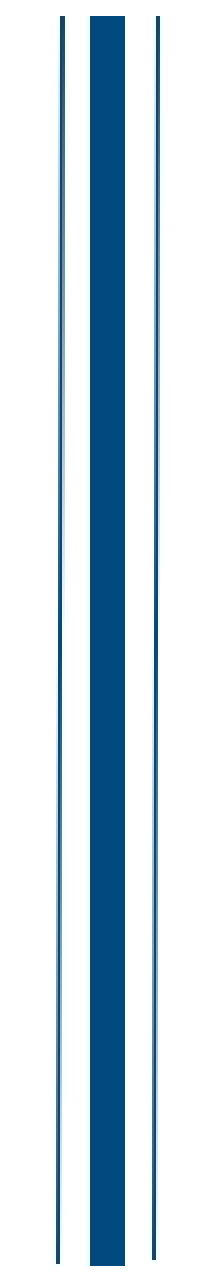
\includegraphics[width=0.5cm,height=15.3cm]{LineaAzul.eps}}
	    \put(-37,-275){\includegraphics[width=3cm,height=2.5cm]{logoescom.eps}}
	\end{picture}}
	\parbox{14cm}{\vspace{1cm} 
	\begin{center}
	    {\fontsize{20}{30}\textbf{ INSTITUTO POLITÉCNICO NACIONAL}}\\[0.2cm]
	    
	    {\fontsize{16}{20} \textbf{ESCUELA SUPERIOR DE CÓMPUTO}}\vspace{1cm}\\[1cm]
	    {\fontsize{20}{20} \textbf{ESCOM}}\vspace{2cm}\\
	    
	    {\fontsize{14}{20} \textit{Trabajo Terminal}}\vspace{1cm}\\
	    {\fontsize{16}{20} \textbf{``Yolotl: un videojuego para fomentar la cultura''}}\vspace{0.5cm}\\
	    {\fontsize{14}{20} \textit{2017-A035}}\vspace{1.5cm}\\
	    {\fontsize{14}{20} \textit{Presentan}}\\
	    {\fontsize{14}{20} \textbf{Hernández Bautista Yasmine Pilar}}\vspace{1cm}\\
	   	{\fontsize{14}{20} \textbf{Márquez Hernández Karla Rocío}}\vspace{1.5cm}\\
	   \fontsize{14}{20} \textit{Directores}\\

	    
	    
{\fboxrule=0pt \fboxsep=6pt	    
\fbox{{\fontsize{14}{20} \textbf{\textit{M. en C. Rafael Norman Saucedo Delgado}}.}\vspace{3.5cm}}
\fbox{{\fontsize{14}{20} \textbf{\textit{Lic. Ulises Vélez Saldaña}}.}\vspace{3.5cm}}}\\[3.5cm]
\end{center}
	    
	    \hfill  \fontsize{12}{20} \textit{Noviembre 2017}
	    
	}
\end{titlepage}

\thispagestyle{empty}

\parbox{18cm}{
\parbox{1.5cm}{
\includegraphics[width=1.5cm,height=2.5cm]{IPN.eps}
}
\parbox{12cm}{
\centering{{\fontsize{16}{0}\textbf{ INSTITUTO POLITÉCNICO NACIONAL}}\\	
{\fontsize{16}{0} \textbf{ESCUELA SUPERIOR DE CÓMPUTO}}}
}
\parbox{1.5cm}{
\includegraphics[width=2.5cm,height=2cm]{logoescom.eps}
}\vspace{1.5cm} 
}

	\begin{center}
	    
	    
\begin{multicols}{2} 
\raggedright{{\fontsize{14}{20} No. de TT:2017-A035}} 

\raggedleft{{\fontsize{14}{20} 17 de noviembre de 2017}}
\end{multicols}\vspace{1cm}

	    {\fontsize{14}{20} \textit{Documento Técnico}}\vspace{1cm}\\
	    {\fontsize{16}{20} \textbf{``Yolotl: un videojuego para fomentar la cultura''}}\vspace{1.5cm}\\
	    {\fontsize{14}{20} \textit{Presentan}}\\
	    {\fontsize{14}{20} \textbf{Hernández Baustista Yasmine Pilar\footnote{daughterofthewind10@gmail.com}}}\vspace{1cm}\\
	    {\fontsize{14}{20} \textbf{Márquez Hernández Karla Rocío\footnote{yolotl.escom@gmail.com}}}\vspace{1cm}\\
	   
	   \fontsize{14}{20} \textit{Directores}\vspace{1.5cm}\\
	    
	    
{\fboxrule=0pt \fboxsep=12pt	    
\fbox{{\fontsize{14}{20} \textbf{\textit{M. en C. Rafael Norman Saucedo Delgado}}.}\vspace{5.5cm}}
\fbox{{\fontsize{14}{20} \textbf{\textit{Lic. Ulises V\'elez Saldaña}}.}
}}
\end{center}
\begin{center}
{\fontsize{14}{20} \textbf{RESUMEN}}
\end{center}
En México la industria de videojuegos tiene una alta demanda de consumo; sin embargo, existen pocos estudios que desarrollen videojuegos basados en la cultura mexicana. Actualmente en México existe un fuerte desinterés en la cultura nacional. El presente trabajo terminal consiste en el desarrollo de un videojuego que fomente la cultura con temática de la cultura mexica. 
\\
 
\textbf{\textit{Palabras clave}}. –  Cultura mexica, desarrollo tecnológico, ingeniería de software, videojuego.
	
	
	%\maketitle
	\tableofcontents
	
	\chapter{Introducción}

%introducción **anteproyecto**
%tema: problema de estudio, teoria asociada con el tema, antecedentes históricos
%objetivo
%alcance
%plan de desarrollo (se divide en x partes)
%valor o importancia del tema (opcional)
%resumir logros (opcional)

En este trabajo el problema de estudio será la ignorancia que existe de la sociedad en México sobre su propia cultura. Para ello definiremos lo que es la cultura y el como toma lugar específicamente en este país. Pues la investigación que se mostrará señala la relación que existe entre el desarrollo social de un país, con el saber que la gente tiene de su propia historia, arte, tradiciones y más conocimiento involucrado que se verá. La información será mostrada en estadísticas y encuestas a lo largo de los años, hasta una comparación reciente. 
\\[1pt]

Para atacar este problema considerarémos como propuesta de solución la creación de un videojuego. Este videojuego no solo deberá cumplir con las características y componentes de un videojuego común, si no también deberá pasar por un proceso llamado gamificación y cumplir con requisitos que ayudarán al nivel de impacto de la solución del problema. Para ello veremos lo que significa un videojuego y los pasos a seguir para el proceso de gamificación.
\\[1pt]

Como antecedentes históricos en el tema de videojuegos, tenemos que desde el año 1952 se tiene registro de elaboración de juegos en medios digitales. como ejemplo en este mismo año se tiene el juego OXO desarrollado por Alexander S. Douglas como proyecto de tesis de su universidad, que consiste en el juego comúnmente conocido aquí como "gato", donde la interacción se daba entre un jugador humano y una máquina. Los primeros juegos tenían como propósito solo el entretenimiento y en cierta medida la investigación de las capacidades de la nueva tecnología que se presentaba en la época, pues por el momento se daban dentro de institutos o centros de estudio. Poco a poco se iban introduciendo nuevos componentes o mejoras a los videojuegos como la interfaz o el hecho de poder involucrar a dos jugadores en un mismo juego y convertirlo en una competición. Después por el año de 1966 los videojuegos empezaron a interactuar con otros dispositivos físicos como el televisor. Así los videojuegos empezaron a adentrarse en el mundo de la industria y comercio, lo que ocasionó una evolución acelerada de los mismos. A partir de los años 1900 es cuando los videojuegos toman el inicio de una fuerte popularidad comercial. Esta popularidad incremento las disciplinas y herramientas para el desarrollo de un videojuego, ocasionando de igual manera la creación de nuevos objetivos de un videojuego, como ejemplo de ello son los videojuegos educativos. Al final, actualmente los videojuegos es una industria que genera más dinero que el cine, toma a cualquier público objetivo y es usado como herramienta, que abarca no solo el entretenimiento. Ahora en vez de ser los videojuegos solo un estudio de la tecnología, los videojuegos se utilizan como apoyo de estudio a otra áreas.    
\\[1pt]

El objetivo consiste en que el videojuego a crear, de una manera divertida insite a los jugadores a un interés mayor al tema de la cultura. No se perderá de vista como elemento principal el entretenimiento del jugador, ya que se quiere de una manera implícita enseñar al jugador historia y mitología de México. El contexto histórico que se tomará será la época prehispánica Méxicana, donde claramente existiran eventos de fantasía para no perder la atención del jugador. Al final el alcance que se busca, es que el jugador se motive a aprender más al respecto y lo mostrado en el juego se haya aprendido en cualquier medida. 
\\[1pt]

Para ello este reporte se divide en una descripción detallada del planteamiento del problema, el marco teórico que cuenta con los temas a entender que son; los videojuegos, su definición, la clasificación que existe, la industria mundial que lo rodea, un estudio de mercado y la industria en México; el desarrollo de videojuegos, las metodologías que existen, que es pipeline, los motores gráficos que se utilizan y el software auxiliar a ocupar; la gamificación, sus características, los tipos de jugadores que existen, el proceso para realizarlo y la finalidad; la cultura; la cultura digital, la división que ha tomado la educación cultural; por último en el marco teórico los videojuegos educativos, después se seguirá con el estado del arte para entender las características del proyecto, el trabajo realizado para ver con lo que se ha encontrado, los resultados obtenidos y al final las observaciones que se tendrán del proyecto.
\\[1pt]

Los videojuegos están dentro de las tecnologías, las cuales están en constante cambio y evolución. Así de igual manera, los medios tecnológicos pueden ayudar a la evolución de otras áreas y problemas actuales. Por ello es importante aprender a usar la tecnología y usarla en beneficio.
\\[1pt]

	\chapter{Planteamiento del problema} 

Hoy en día en México, la sociedad no tiene ningún interés por conocer o realizar actividades culturales. Tomaremos como actividades culturales a aquellas de aspecto artístico o histórico como obras de arte, literatura, música, danza, exposiciones y proyecciones audiovisuales. A continuación hablarémos sobre el contexto que rodea esta problemática, sus causas, consecuencias y la solución que proponemos.
\\[1pt]

\section{Contexto}
La diversidad cultural según el Movimiento Nacional por la Diversidad Cultural de México(MNDCM) es la múltiple cantidad de formas de expresión entre grupos y sociedades\cite{pp05}. La diversidad se manifiesta a través de distintos modos de creación artística, producción, difusión y distribución de dichas expresiones. La diversidad cultural es vital para el desarrollo de cualquier comunidad, pues es fuente de creatividad, innovación, originalidad, intercambio y enriquecimiento.
\\[1pt]

México es conocido por ser un país muy diverso culturalmente hablando. Cada estado posee su propia cultura regional, como la música, vestimenta tradicional, comida, entre otras cosas. Entre todos los estados del país podemos ver que existen grandes diferencias y aún así se comparte una misma identidad como país.
\\[1pt]

\section{Causas}

La ignorancia cultural del país se debe a que existe un desconocimiento de desarrollo social. Es decir que la sociedad del país tampoco tiene idea sobre su situación económica, capital humano, condiciones de salud, estado de la educación y condiciones de vida, todo esto llamado comúnmente como el bienestar social.
\\[1pt]

Existe una relación directa entre el desarrollo cultural y social. Pues ambas son debido al entorno y evolución de la sociedad que involucra. Con lo anterior deducimos que el desarrollo social favorece el desarrollo cultural.
\\[1pt]

En la última encuesta de Ipsos sobre Percepción\cite{pp04} se revela que tan errónea es la interpretación que las personas tienen sobre su desarrollo social. A partir de los datos recogidos en la encuesta y su comparación con datos reales, en temas acerca de los problemas y rasgos clave de la población de su país se elaboró la gráfica \ref{fig:ipso}. Se puede observar que México ocupa el duodécimo lugar (empatado con Corea del sur) en ignorancia total de su desarrollo como país. Entonces sí existe una ignorancia sobre desarrollo social en México.
\\[1pt]

\begin{figure}
	\centering 
	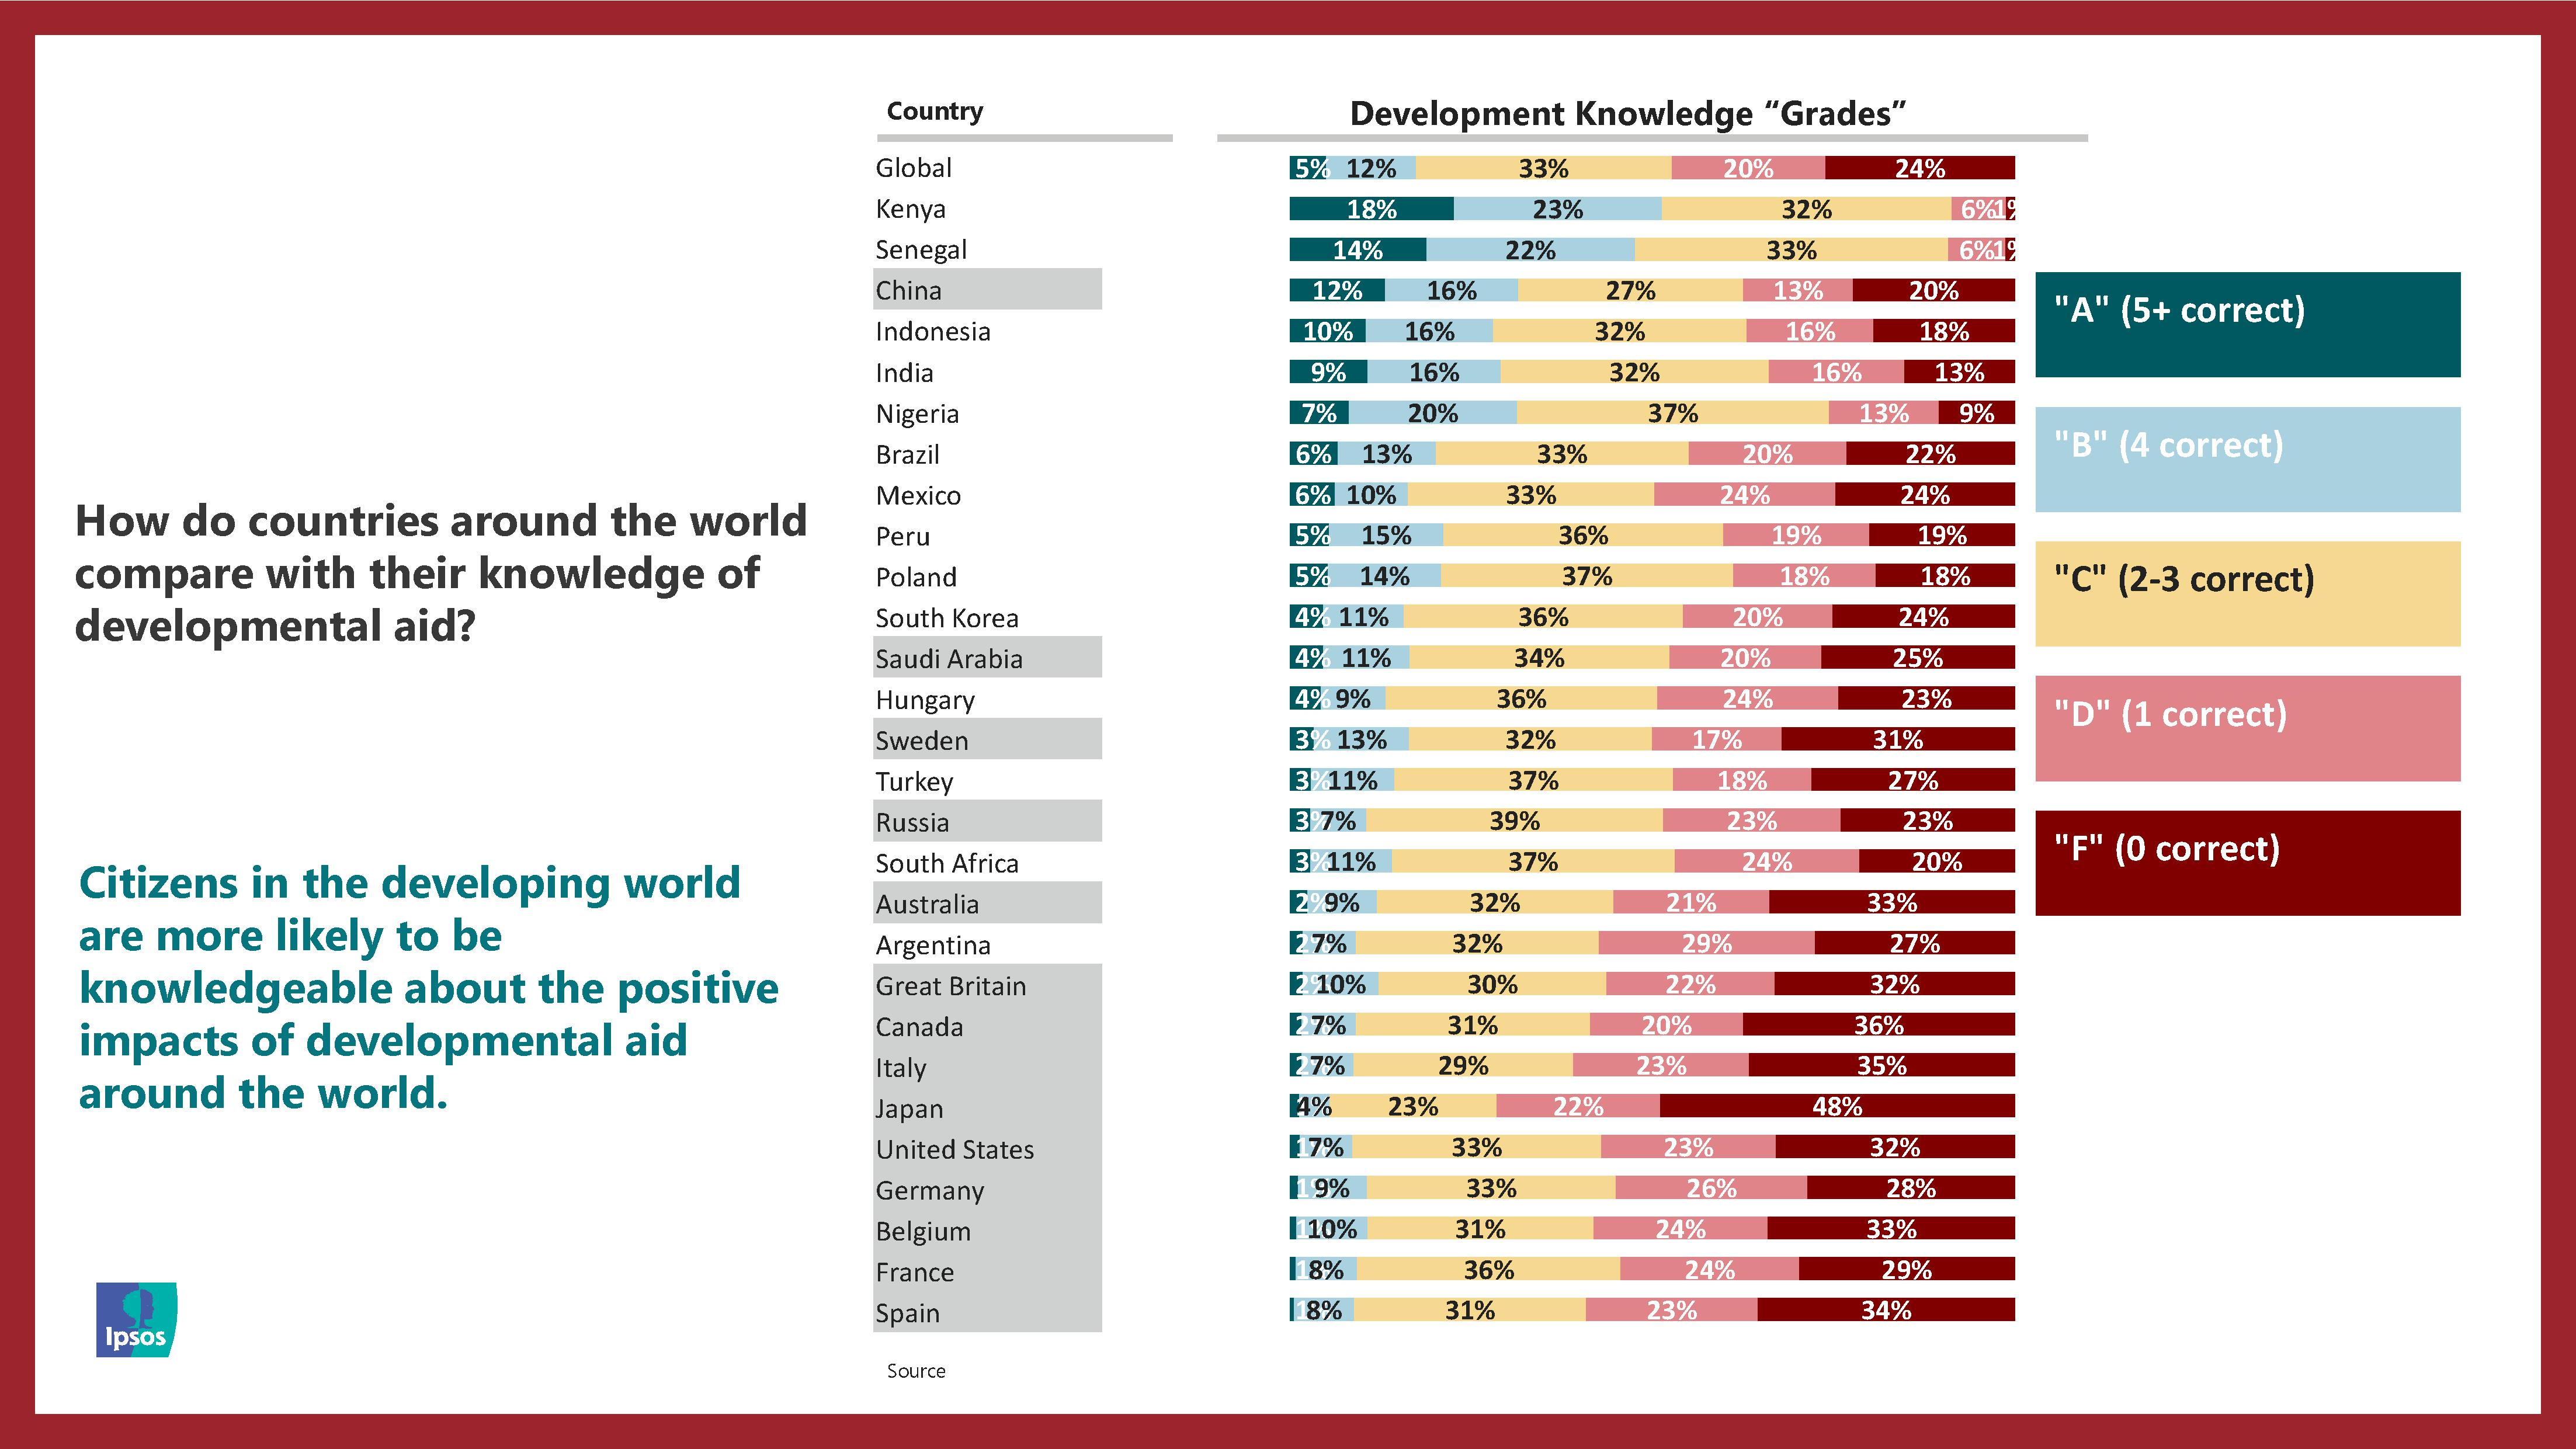
\includegraphics[width=\textwidth]{03MarcoTeorico/imageR/ipso}
	\caption{Gráfica global de la percepción de 28 paises respecto a la realidad. Donde vemos una gráfica que representa la cantidad de aciertos que tuvo la población por país en relación a la realidad.[Imagen](2017, Septiembre). Recuperado de https://www.ipsos.com/sites/default/files/ct/news/documents/2017-09/Gates\_Perils\_of\_Perception\_Report-September\_2017.pdf}
	\label{fig:ipso}
\end{figure}

\section{Consecuencias}
Ya que el desarrollo social y cultural están ligados, estos se encuentran también dependientes el uno del otro para su impulso. El movimiento cultural no solo favorecer el desarrollo recreativo si no que impulsa el desarrollo de sus naciones y viceversa. Tenemos como ejemplo en otros países del mundo, donde han sabido valorar las costumbres y tradiciones, he ahí donde nace el orgullo por su patria y se convierten en nacionalistas, demostrando el amor por su pueblo, marcando de manera definitiva el desarrollo científico, político y social de su nación\cite{pp06}.
\\[1pt]

La ignorancia cultural es el principal elemento que permite la injusticia, la enajenación y la explotación. Este fenómeno es sumamente grave y perjudicial para conformar lo que es la Identidad Cultural, la Identidad Nacional y la conciencia de la Nación. Al no saber quién es, cuáles son sus orígenes, su historia, su legado, su nombre, sus valores y principios, se le condena a la sociedad a permanentemente estar exaltando lo ajeno y despreciando lo propio.
\\[1pt]

En 2017, 41\% de los mexicanos no fue a ninguna actividad cultural según INEGI\cite{pp02}. La cifra podría leerse al revés: donde el 59\% del total de la población de 18 y más años de edad declaró que asistió a algún evento cultural seleccionado en los últimos doce meses. Pero cuando se trata de un país con una intensa vida cultural y artística, con más de 1,300 museos, alrededor de 178 zonas arqueológicas abiertas al público, 641 teatros y más de 4,000 salas de cine, de acuerdo con datos de la propia Secretaria de Cultura del gobierno federal\cite{pp01} al final queda que cuatro de cada diez personas no tienen como hábito la cultura a pesar de que varios de ellos son gratuitos.
\\[1pt]

Como ejemplo de la decadente autoconciencia cultural en México tenemos el día de la independencia. Quizá podría pensarse que todos los mexicanos saben que se festeja el 15 y 16 de septiembre. Sin embargo, los datos de la encuesta telefónica de Parametría\cite{pp03} muestran que 11\% de las personas no tiene idea de lo que se conmemora como se ve en la gráfica \ref{fig:enc01} y 57\% no sabe de que país se independizó como se ve en la gráfica \ref{fig:enc02}. Adicionalmente como podría esperarse, el nivel de escolaridad influye en el conocimiento que se tiene sobre el tema. Así, puede observarse que conforme aumenta el nivel de escolaridad se incrementa el conocimiento sobre la celebración de independencia y también sobre el país del cual se independizó México según la gráfica. \ref{fig:enc03}.
\\[1pt]

\begin{figure}
	\centering 
	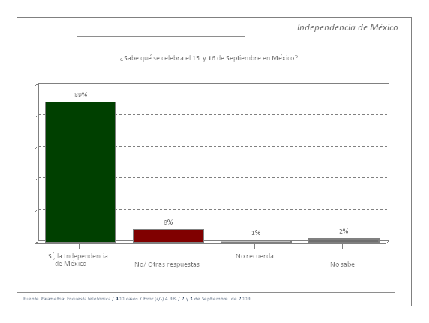
\includegraphics[width=.50\textwidth]{03MarcoTeorico/imageR/enc01}
	\caption{Gráfica a la pregunta ¿Sabe que se celebra el 15 y 16 de Septiembre en México?[Imagen](2009, Septiembre). Recuperado de: http://www.parametria.com.mx/carta\_parametrica.php?cp=4170.}
	\label{fig:enc01}
\end{figure}

\begin{figure}
	\centering 
	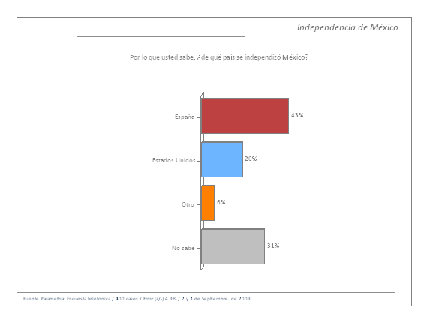
\includegraphics[width=.5\textwidth]{03MarcoTeorico/imageR/enc02}
	\caption{Gráfica a la pregunta ¿De que país se independizó México?[Imagen](2009, Septiembre). Recuperado de: http://www.parametria.com.mx/carta\_parametrica.php?cp=4170.}
	\label{fig:enc02}
\end{figure}

\begin{figure}
	\centering 
	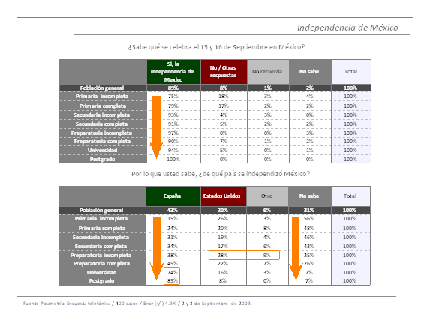
\includegraphics[width=.5\textwidth]{03MarcoTeorico/imageR/enc03}
	\caption{Gráfica de como influye la escolaridad en el conocimiento que se tiene de las fiestas patrias[Imagen](2009, Septiembre). Recuperado de: http://www.parametria.com.mx/carta\_parametrica.php?cp=4170.}
	\label{fig:enc03}
\end{figure}

Debemos saber cuál es nuestra verdadera herencia cultural y cuál nuestro legado, para preservarlo y desarrollarlo. Y como dice Guillermo Marín \cite{pp07} ``Este país se tiene que encontrar a sí mismo".
\\[1pt]


\section{Propuesta de solución}
Propondremos como solución el crear un videojuego con contexto histórico y mitológico del país prehispánico mexicano. Para esto el factor de entretenimiento y diversión lo sobrepondremos al del conocimiento o educativo.
\\[1pt]

%%%%%%%%%%%%%%%%%%%%%%%%%5YA EXISTE?
Como ejemplo similar tomaremos el videojuego llamado ``Assasins Creed II" lanzado en el año 2009, que debutó en el puesto número 1 en Estados Unidos, Canadá, Suecia, Francia, España y Australia, y dentro del «Top 50» en más de diez países. Este juego tiene como género acción-aventura, también se situa en la época renacentista y este hecho lográ que el jugador adquiera conocimientos sobre ese tiempo, tanto lugares, como personas, situación social, etc.
\\[1pt]

%%%%%%%%%%%%%%%%%%%%%%%%%%55QUE IMPLICA?
Para llevar a cabo el diseño de un videojuego los programadores son los responsables de hacer posible la interactividad entre el jugador y el sistema. Se realizará detro del proyecto la programación estructurada, orientada a objetos, modelado, arte digital, conocimiento de dispositivos móviles y animación digital. Considerando importante usar modelos matemáticos para las diferentes experiencias de juego. 
\\[1pt]

%%%%%%%%%%%%%%%%%%%%%%%%%%%%%%%VENTAJAS?
El resultado de adquisición de conocimiento en lo videojuegos se debe al cómo. En la imagen \ref{fig:conoAprendizaje} se muestra el cono de la experiencia de Edgar Dale (pedagogo) donde resaltamos que el mayor aprendizaje es por medio de la simulación.

\begin{figure}
	\centering 
	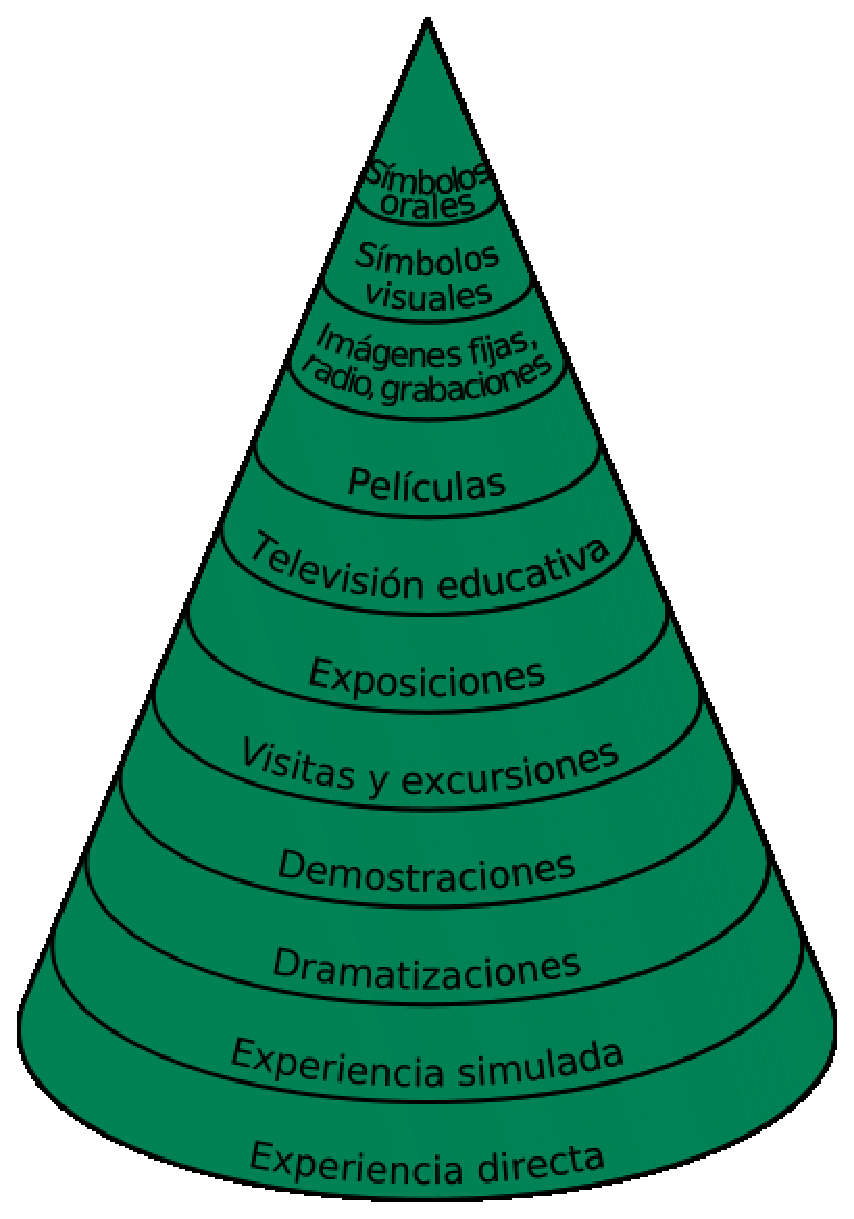
\includegraphics[width=.5\textwidth]{03MarcoTeorico/imageR/conoAprendizaje}
	\caption{Cono de la experiencia de Edgar Dale. Se muestra diferentes maneras de aprendizaje que se ordenan según su impacto de aprendizaje.[Imagen](2008). Recuperado de: https://es.wikipedia.org/wiki/Edgar\_Dale\#/media/File:Cono\_de\_la\_Experiencia.svg}
	\label{fig:conoAprendizaje}
\end{figure}

Los medios audiovisuales son los que mayor impacto tiene en difusión cultural como se ve en la gráfica de la imagen \ref{fig:modecult}. Así podemos ver una potencial herramienta para insitar a la participación en los eventos culturales, pues los videojuegos son medios audiovisuales.
\\[1pt]

\begin{figure}
	\centering 
	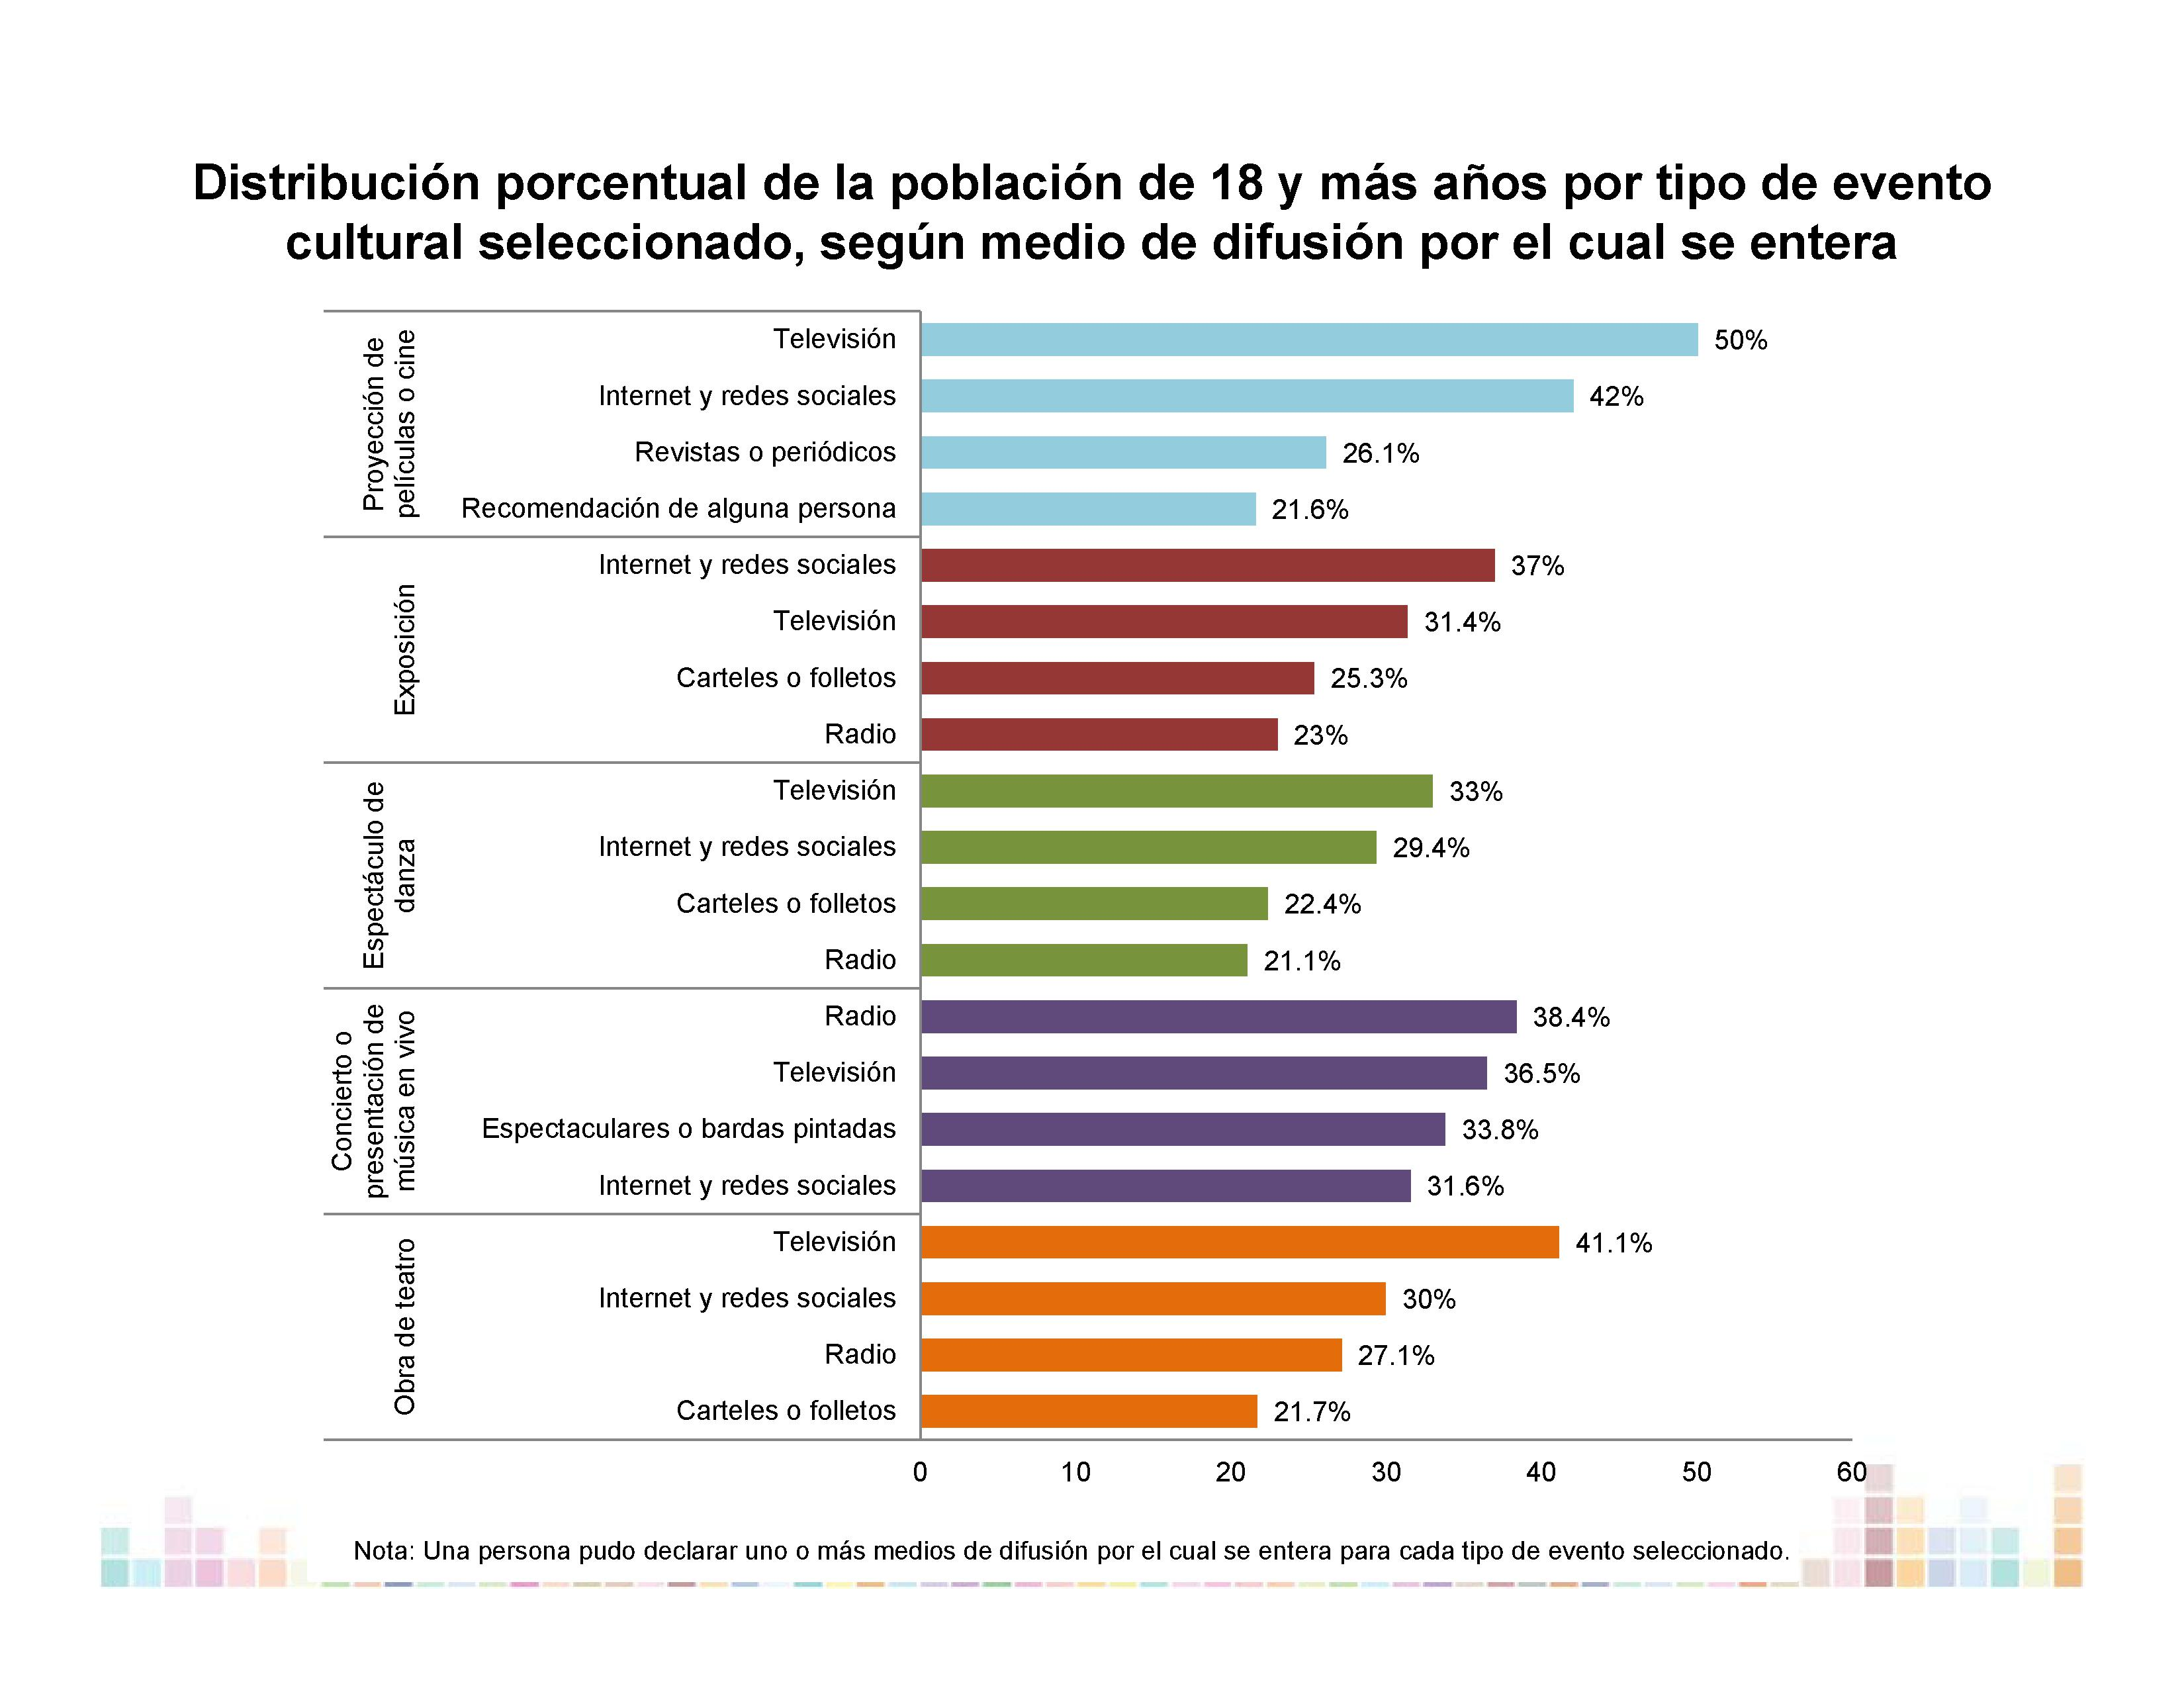
\includegraphics[width=.75\textwidth]{03MarcoTeorico/imageR/modecult}
	\caption{Encuesta MODECULT en asistencia por tipo de evento y medio de difusión por el cual se ha enterado.[Imegen](2017, Mayo). Recuperado de: http://internet.contenidos.inegi.org.mx/contenidos/productos/prod\_serv/contenidos/espanol/bvinegi/productos/nueva\_estruc/promo/resultados\_modecult\_may2017.pdf}
	\label{fig:modecult}
\end{figure}

También otra de las ventajas es la cantidad de gente que juega videojuegos en México y el dispositivo por el cuál lo consumen como lo muestra la imagen \ref{fig:consumo30}. Donde el 20\% de los mexianos consumen videojuegos y 45\% de ellos se juegan en dispositivos móviles.

\begin{figure}
	\centering 
	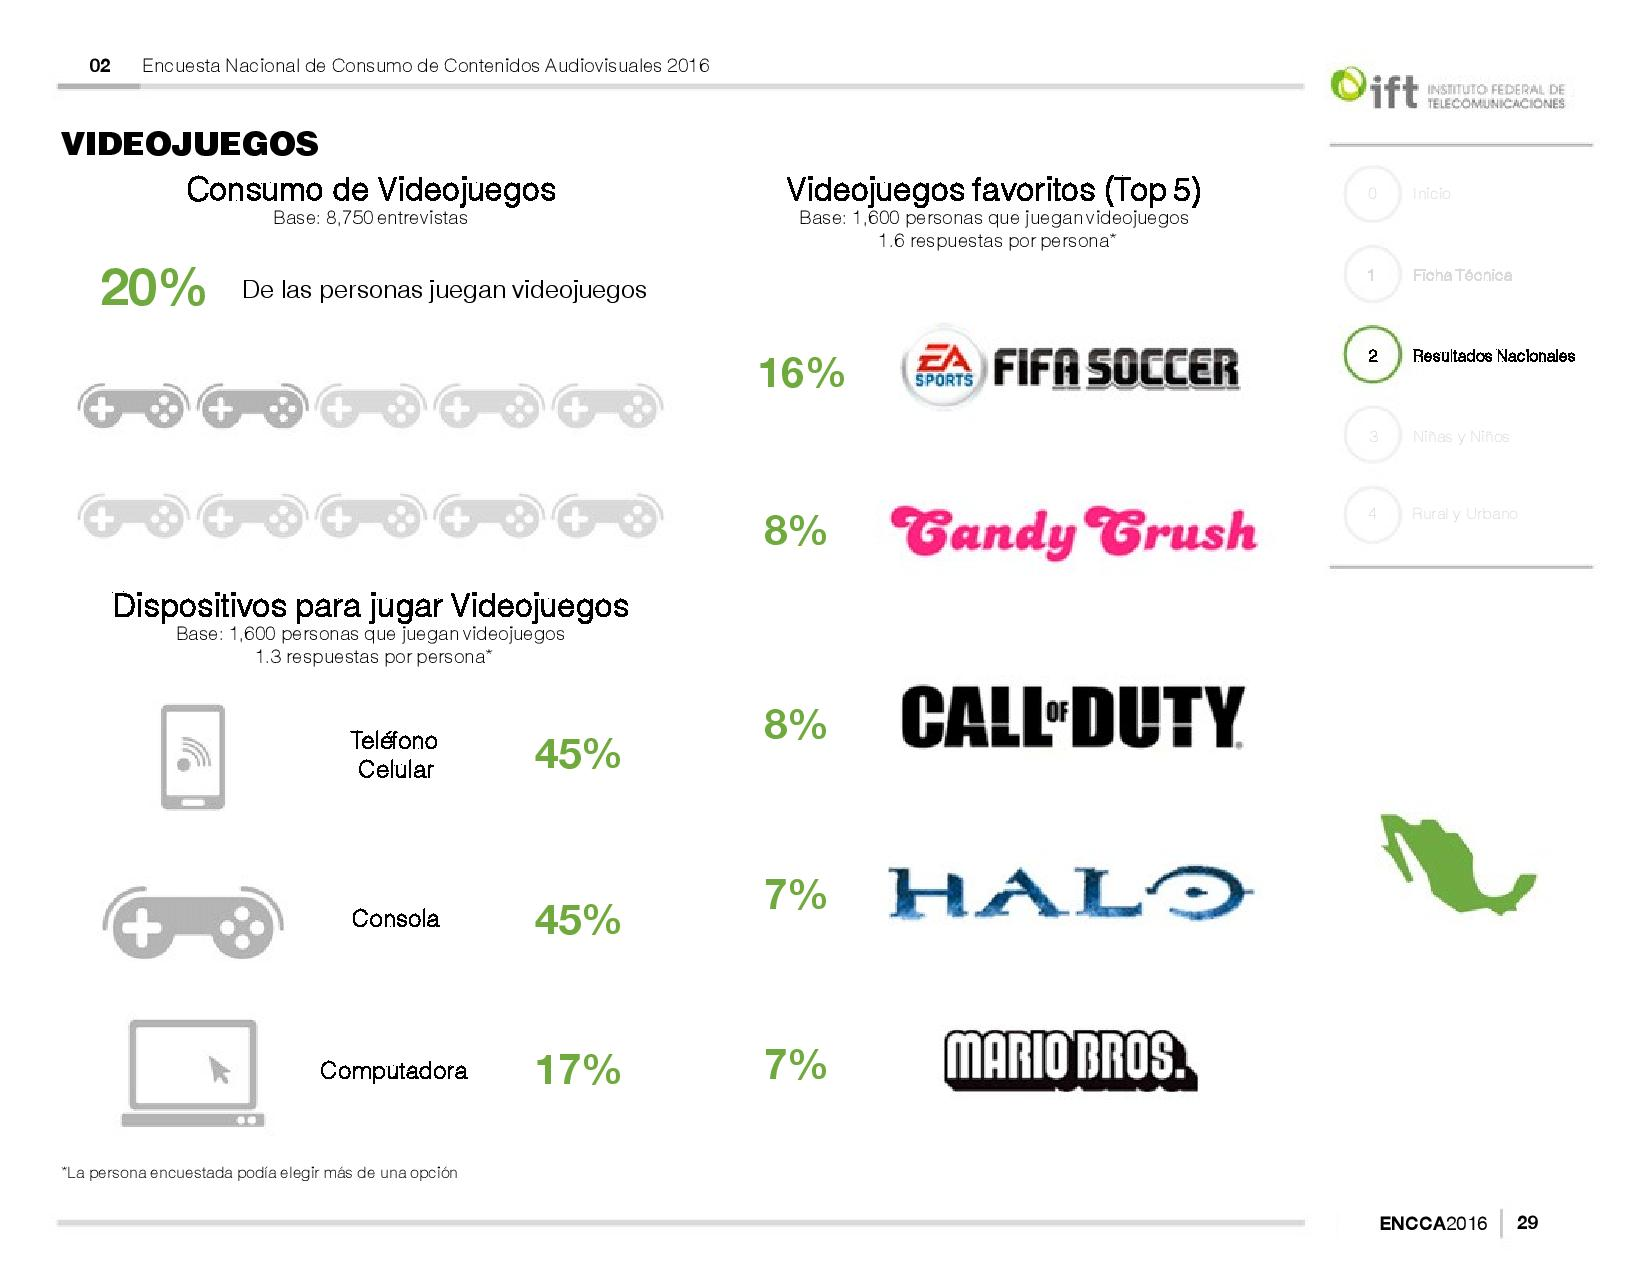
\includegraphics[width=.75\textwidth]{03MarcoTeorico/imageR/consumo30}
	\caption{Encuesta Nacional de Consumo de Contenidos Audiovisuales, donde muestra el consumo de videojuegos[Imegen](2016). Recuperado de: http://www.ift.org.mx/sites/default/files/encca2016\_vf-compressed.pdf}
	\label{fig:consumo30}
\end{figure}

%%%%%%%%%%%%%%%%%%%%%%%%%%DESVENTAJAS?

Una desventaja de los videojuegos en cuestión de desarrollo es que son un complejo sistema tecnológico que combina diversos elementos: visuales, matemáticos, físicos, electrónicos o narrativos, entre otros muchos para generar una experiencia controlada porel jugador para su mayor entretenimiento. Por tanto existe una complejidad al unir de forma adecuada todos esos elemntos para crear una gran experiencia de diversión para los jugadores, se necesita de una gran cantidad de talentos diversos o multidisciplinarios, los cuales no se abarcarán todos ellos.

También se debe tomar en cuenta que existe una gran cantidad de gustos e intereses entre los jugadores existentes y no se puede aplicar todos los existentes.

La mejora de las condiciones de un producto en un videojuego resulta esencial. Por esta misma razón el tiempo de desarrollo siempre es muy largo y en la mayoría de las ocasiones tiene muchos contratiempos que provocan retrasos de lanzamiento o incluso rediseños completos.




	\chapter{Marco teórico conceptual}
	\section{Videojuego}
En este apartado se dará la definición de un videojuego y aquello que involucra, la clasificación que existe para ellos, como se encuentra en la actualidad la industrial mundial del videojuego, luego de manera específica un pequeño estudio de mercado en México con solo los campos que nos interesan para el proyecto y finalmente el desarrollo que existe de los videojuegos dentro de la industria en México. 

\subsection{Definición}
Un videojuego es un medio de entretenimiento que involucra a un usuario, denominado jugador, en una interacción constante entre una interfaz y un dispositivo de video según Morales Urrutia\cite{defVid}. Los videojuegos recrean	entornos y situaciones virtuales en los que el jugador puede controlar la situación para alcanzar objetivos por medio de determinadas reglas. La interacción se lleva a cabo mediante dispositivos de salida y de entrada.
\\[1pt]
		
Los videojuegos arte, ciencia y tecnología; involucran una gran cantidad de habilidades y conocimientos en distintas disciplinas, desde ciencias formales hasta ciencias sociales que van más allá del típico proyecto de software e implican al mismo tiempo la creatividad y la imaginación.
\\[1pt]

Su propósito de igual manera es muy variado, puede ser con fines solo de entretenimiento, aprendizaje, simulación, terapia física o emocial, y más. El propósito de un videojuego puede ser siempre definido, pero tambien puede tener como consecuencia otros resultados benéficos o no.
\\[1pt]

Ya que los propósitos de un videojuego dependen del enfoque que se le quiera dar, nos tenemos que apoyar a quien va dirigido nuestro contenido. Un videojuego puede ir dirigido a cualquier persona, esto determinará después los elementos u objetivos que se quieren conseguir.
\\[1pt]  
					
\subsection{Clasificación}
La clasificación es un proceso que permite una ordenación de elementos, según determinados criterios. Así se reunen en grupos que comparten características similares con fines de organización y facilitar la comunicación respecto de un tema. Primero hablaremos de las clasificaciones que se estan discutiendo para los videojuegos y después según las necesidades del proyecto tomaremos las convenientes. 
\\[1pt]

El documento MDA\cite{vid10} (por sus siglas en inglés) establece los tres aspectos fundamentales, Mecánicas, Dinámicas y Estética como un marco de referencia para entender los juegos y hacer una mejor clasificación de ellos. Las mecánicas, son las reglas y sistemas que crean nuestra experiencia de juego, sus componentes particulares a nivel representación de datos y algoritmos; las dinámicas, describen el comportamiento de las mecánicas en respuesta a las acciones del jugador; y la estética, define la respuesta emocional evocada por el usuario cuando interactúa con el juego. Aunque esta clasificación abarca a todos los videojuegos existentes, no son considerados comúnmente en la industria, por esa razón no se tomará dicha clasificación.
\\[1pt]

Mark Wolf\cite{vid11} enfatiza la diferencia fundamental de los videojuegos con otros medios y el por qué de ser necesaria una categorización en géneros muy distinta a la aplicable a libros y películas. Pues la participación del jugador es el determinante a la hora de describir y clasificar juegos de video. Mark Wolk comenta que "Por supuesto, cualquier sistema propuesto será objeto de debate y crítica. Al mismo tiempo, aparecer con un listado consistente y comprensivo que intenta definir y articular las fronteras de cada uno, es una tarea mucho más difícil que criticar otros ya existentes". Donde se vuelve a comentar el problema de la no existencia de una clasificación determinada para los videojuegos.
\\[1pt]

Así que, se abarcarán dos de las clasificaciones determinadas por el mercado de la industria. La clasificación por contenido, que son definidas por asuntos legales que competen a cada región y la clasificación por géneros que son las razones emotivas o de experiencia que tenemos dentro del videojuego.
\\[1pt]

\subsubsection{Clasificación por contenido}

	Es usado para el control y supervisión de contenido y asi determinar el público al cual puede ser mostrado.  Existen diferentes sistemas en el mundo donde la mayoría de estos están asociados y patrocinados por un gobierno y a veces forman parte del sistema de clasificación de películas del país.Existen hasta el momento diecinueve tipos diferentes de clasificación por contenido.\\[1pt]	
	
	México pertenece a la Junta de Clasificación de Software de Entretenimiento (ESRB, Entertainment Software Rating Board)\cite{vid02}. La pertenencia a esta clasificación se debe a la cercanía con EUA que tiene el país y el constante comercio que comparten. Esta clasificación proporciona una información concisa y objetiva acerca del contenido de los juegos de video y las aplicaciones para que los consumidores, en especial los padres, puedan tomar decisiones informadas. La clasificación de la ESRB constan de tres partes; edad, descriptor de contenido y elementos interactivos.\\[1pt]
			
\textbf{Por edad}
\\[1pt]
En donde se sugieren la edad adecuada para el juego. La imagen \ref{fig:clasEti} muestra la simbología usada por edad. Esta representación es usada tal cuál en los empaques del videojuego. A continuación se enlistan los apartados por edad que existen y a que público pertenecen.	
\\[1pt]

	\begin{figure}
	\centering 
	
\includegraphics[width=\textwidth]{03MarcoTeorico/imageR/clasEti}
	\caption{Etiquetas de clasificación por edad en un videojuego.}
	\label{fig:clasEti}
\end{figure}


			\begin{itemize}
			\item Niños pequeños: 
			El contenido está dirigido a niños pequeños menores de diez años.
			
			\item Todos: 
			El contenido por lo general es apto para todas las edades. Puede que contenga una cantidad mínima de violencia de caricatura, de fantasía o ligera, o uso poco frecuente de lenguaje moderado.
			
			\item Todos +10: 
			El contenido por lo general es apto para personas de diez años o más. Puede que contenga más violencia de caricatura, de fantasía o ligera, lenguaje moderado o temas mínimamente provocativos.
			
			\item Adolescentes: 
			El contenido por lo general es apto para personas de trece años o más. Puede que contenga violencia, temas insinuantes, humor grosero, mínima cantidad de sangre, apuestas simuladas o uso poco frecuente de lenguaje fuerte.
			
			\item Maduro: 
			El contenido por lo general es apto para personas de diecisiete años o más. Puede que contenga violencia intensa, derramamiento de sangre, contenido sexual o lenguaje fuerte.
			
			\item Adultos únicamente: 
			El contenido es apto sólo para adultos de dieciocho años o más. Puede que incluya escenas prolongadas de violencia intensa, contenido sexual gráfico o apuestas con moneda real.
			
			\item Clasificación pendiente: 
			Aparece solo en material de publicidad, de comercialización y promocional en relación con un videojuego "en caja" que se espera que lleve una clasificación de la ESRB y debe reemplazarse por la clasificación del juego una vez que haya sido asignada.
			
		\end{itemize}		
			
			\textbf{Descriptores de contenido: } 
			\\[1pt]
			Indican los elementos que pueden haber motivado la clasificación asignada y pueden resultar de interés o preocupación para el comprador. La imagen \ref{fig:clasDes} muestra una etiqueta con los descriptores en una etiqueta a lado de la edad sugerida. A continuación se enlistan los descriptores de contenido que existen al momento y en breve una explicación. 
			\\[1pt]
				\begin{figure}
				\centering
				
\includegraphics[width=0.3\textwidth]{03MarcoTeorico/imageR/clasDes}
				\caption{Muestra de descriptor de contenido de un videojuego.}
				\label{fig:clasDes}
			\end{figure}
			
			
			\begin{itemize}
				\item Referencia al alcohol: Referencia e imágenes de bebidas alcohólicas.
				\item Animación de sangre: Representaciones decoloradas o no realistas de sangre.
				\item Sangre: Representaciones de sangre.
				\item Derramamiento de sangre: Representaciones de sangre o mutilación de partes del cuerpo.
				\item Violencia de caricatura: Acciones violentas que incluyen situaciones y personajes caricaturescos. Puede incluir violencia en la cual un personaje sale ileso después de que la acción se llevó a cabo.
				\item Travesuras cómicas: Representaciones o diálogo que impliquen payasadas o humor sugestivo.
				\item Humor vulgar: Representaciones o diálogo que implique bromas vulgares.
				\item Referencia a drogas: Referencia o imágenes de drogas.
				\item Violencia de fantasía: Acciones violentas de naturaleza fantástica que incluyen personajes humanos y no humanos en situaciones que se distinguen con facilidad de la vida real.
				\item Violencia intensa: Representaciones gráficas y de apariencia realista de conflictos físicos. Puede comprender sangre excesiva o realista, derramamiento de sangre, armas y representaciones de lesiones humanas y muerte.
				\item Lenguaje: Uso de lenguaje inadecuado de moderado a intermedio.
				\item Letra de canciones: Referencias moderadas de lenguaje inadecuado, sexualidad, violencia, alcohol o uso de drogas en la música.
				\item Humor para adultos: Representaciones o diálogo que contienen humor para adultos, incluidas las alusiones sexuales.
				Desnudez: Representaciones gráficas o prolongadas de desnudez.
				\item Desnudez parcial: Representaciones breves o moderadas de desnudez.
				\item Apuestas reales: El jugador puede apostar, incluso colocar apuestas con dinero o divisas de verdad.
				\item Contenido sexual: Representaciones no explícitas de comportamiento sexual, tal vez con desnudez parcial.
				\item Temas sexuales: Alusiones al sexo o a la sexualidad.
				\item Violencia sexual: Representaciones de violaciones o de otros actos sexuales violentos.
				\item Apuestas simuladas: El jugador puede apostar sin colocar apuestas con dinero o divisas reales.
				\item Lenguaje fuerte: Uso explícito o frecuente de lenguaje soez.
				Letra de canciones fuerte: Alusiones explícitas o frecuentes de lenguaje inadecuado, sexo, violencia o uso de alcohol o drogas en la música.
				\item Contenido sexual fuerte: Alusiones explícitas o frecuentes de comportamiento sexual, tal vez con desnudez.
				\item Temas insinuantes: Referencias o materiales provocativos moderados.
				\item Referencia al tabaco: Referencia o imágenes de productos de tabaco.
				\item Uso de alcohol: Consumo de alcohol o bebidas alcohólicas.
				\item Uso de drogas: Consumo o uso de drogas.
				\item Uso de tabaco: Consumo o uso de productos de tabaco.
				\item Violencia: Escenas que comprenden un conflicto agresivo. Pueden contener desmembramiento sin sangre.
				Referencias violentas: Alusiones a actos violentos.
			\end{itemize}
			
			\textbf{Elementos interactivos: } 
			\\[1pt]
			Informan acerca de los aspectos interactivos de los productos, incluida la capacidad de los usuarios de interactuar, o si se comparte la ubicación de los usuarios con otros usuarios. La imagen \ref{fig:clasInt} da como ejemplo en una caja de videojuegos como se vería. 
			\\[1pt]
			
				\begin{figure}
				\centering
				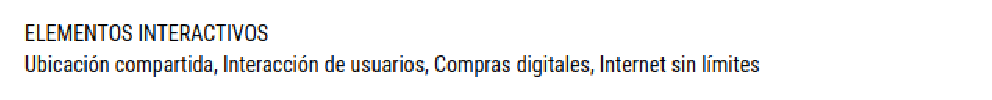
\includegraphics[width=0.5\textwidth]{03MarcoTeorico/imageR/clasInt}
				\caption{Ejemplo de como se muestra los elementos interactivos en el empaque de un videojuego.}
				\label{fig:clasInt}
				\end{figure}
			
			
			\begin{itemize}
			
			\item Ubicación compartida: Incluye la capacidad de mostrar la ubicación del usuario a otros usuarios de la aplicación.
			\item Interacción de usuarios: Indica una posible exposición a contenido sin filtro y sin censura generado por usuarios, que incluye comunicaciones y medios compartidos de usuario a usuario a través de medios y redes sociales.
			\item Compras digitales: Permite la compra de productos digitales directamente desde la aplicación.
			\item Internet sin límites: El producto brinda acceso a Internet.
		\end{itemize}
		
	\subsubsection{Clasificación por género}
 La clasificación por géneros se conforman en torno a factores como: la representación gráfica, el tipo de interacción entre el jugador y la máquina, la ambientación, y su sistema de juego, siendo este último el criterio más habitual a tener en cuenta. A lo largo de la historia de los videojuegos, sus creadores han ido dando lugar a una variedad creciente de géneros en las distintas plataformas disponibles y muchas de la veces son combinables entre sí. Por lo dicho anteriormente de la clasificación, existen diferentes divisiones y subdivisiones por varios autores. A continuación se presenta una de ellas en la imagen \ref{fig:vidGen} por Luis Chong y que a nuestra consideración se tomará.
	\\[1pt]
	
	\begin{figure}
		\centering
		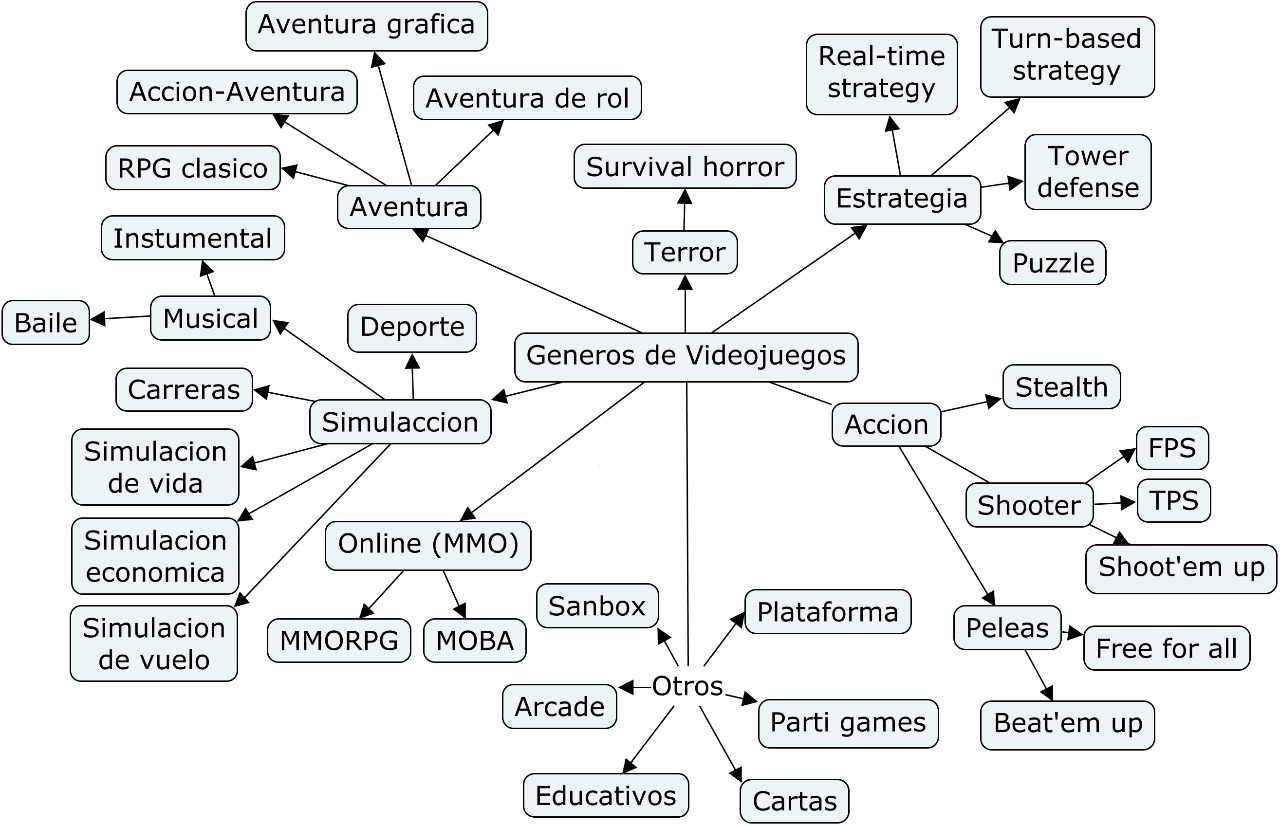
\includegraphics[width=\textwidth]{03MarcoTeorico/imageR/gene}
		\caption{Géneros de videojuegos propuesto por Luis Chong[Imagen](2015). Recuperado de: https://www.emaze.com/@AFRICWZL/Tesis-Artes-Digitales.}
		\label{fig:vidGen}
	\end{figure}	
	
		
\subsection{Industria mundial}
			 
			 La industria mundial refleja el nivel de consumo que existe. El videojuego surge en 1952; no obstante, el videojuego como industria surgiría hasta 1972, logrando su mayor revolución durante la década de los 80`s. 
			 \\[1pt]
			 
			 Según un estudio elaborado por la empresa Newzoo en la imagen \ref{fig:newzooIndMun}, la industria del videojuego generará 108.900 millones de dólares de ingresos totales, de los que se espera que hasta 94.400 millones corresponden solamente a ventas digitales, que representa un 87\% del mercado mundial. Actualmente la industria del videojuego, también llamada industria del ocio virtual, es la industria del entretenimiento, superando a la industria del cine y la música. Ya que hemos visto el consumo de videojuegos ahora nos vamos a su plataforma que nos interesa, que son los dispositivos móviles.
			 \\[1pt]	
			 
			 El segmento de los dispositivos móviles (Smartphones y tablets) es el que aporta más dinero en la industria del videojuego. Este sector copa un 42\% del mercado y su consumo ha tenido un crecimiento del 19\% con respecto al año anterior. Se espera que generen un ingreso de 46.100 millones de dólares. A día de hoy no se entiende a ninguna persona sin su Smartphone en la mano y esto hace que un gran porcentaje de usuarios juegue a algún tipo de juego en su teléfono y hasta utilice navegadores de internet sin necesidad de instalar nada. Se espera que en 2020 acaparen el 50\% del mercado. \cite{vid01}
			 \\[1pt]   
			 
			 	\begin{figure}
			 	\centering
			 	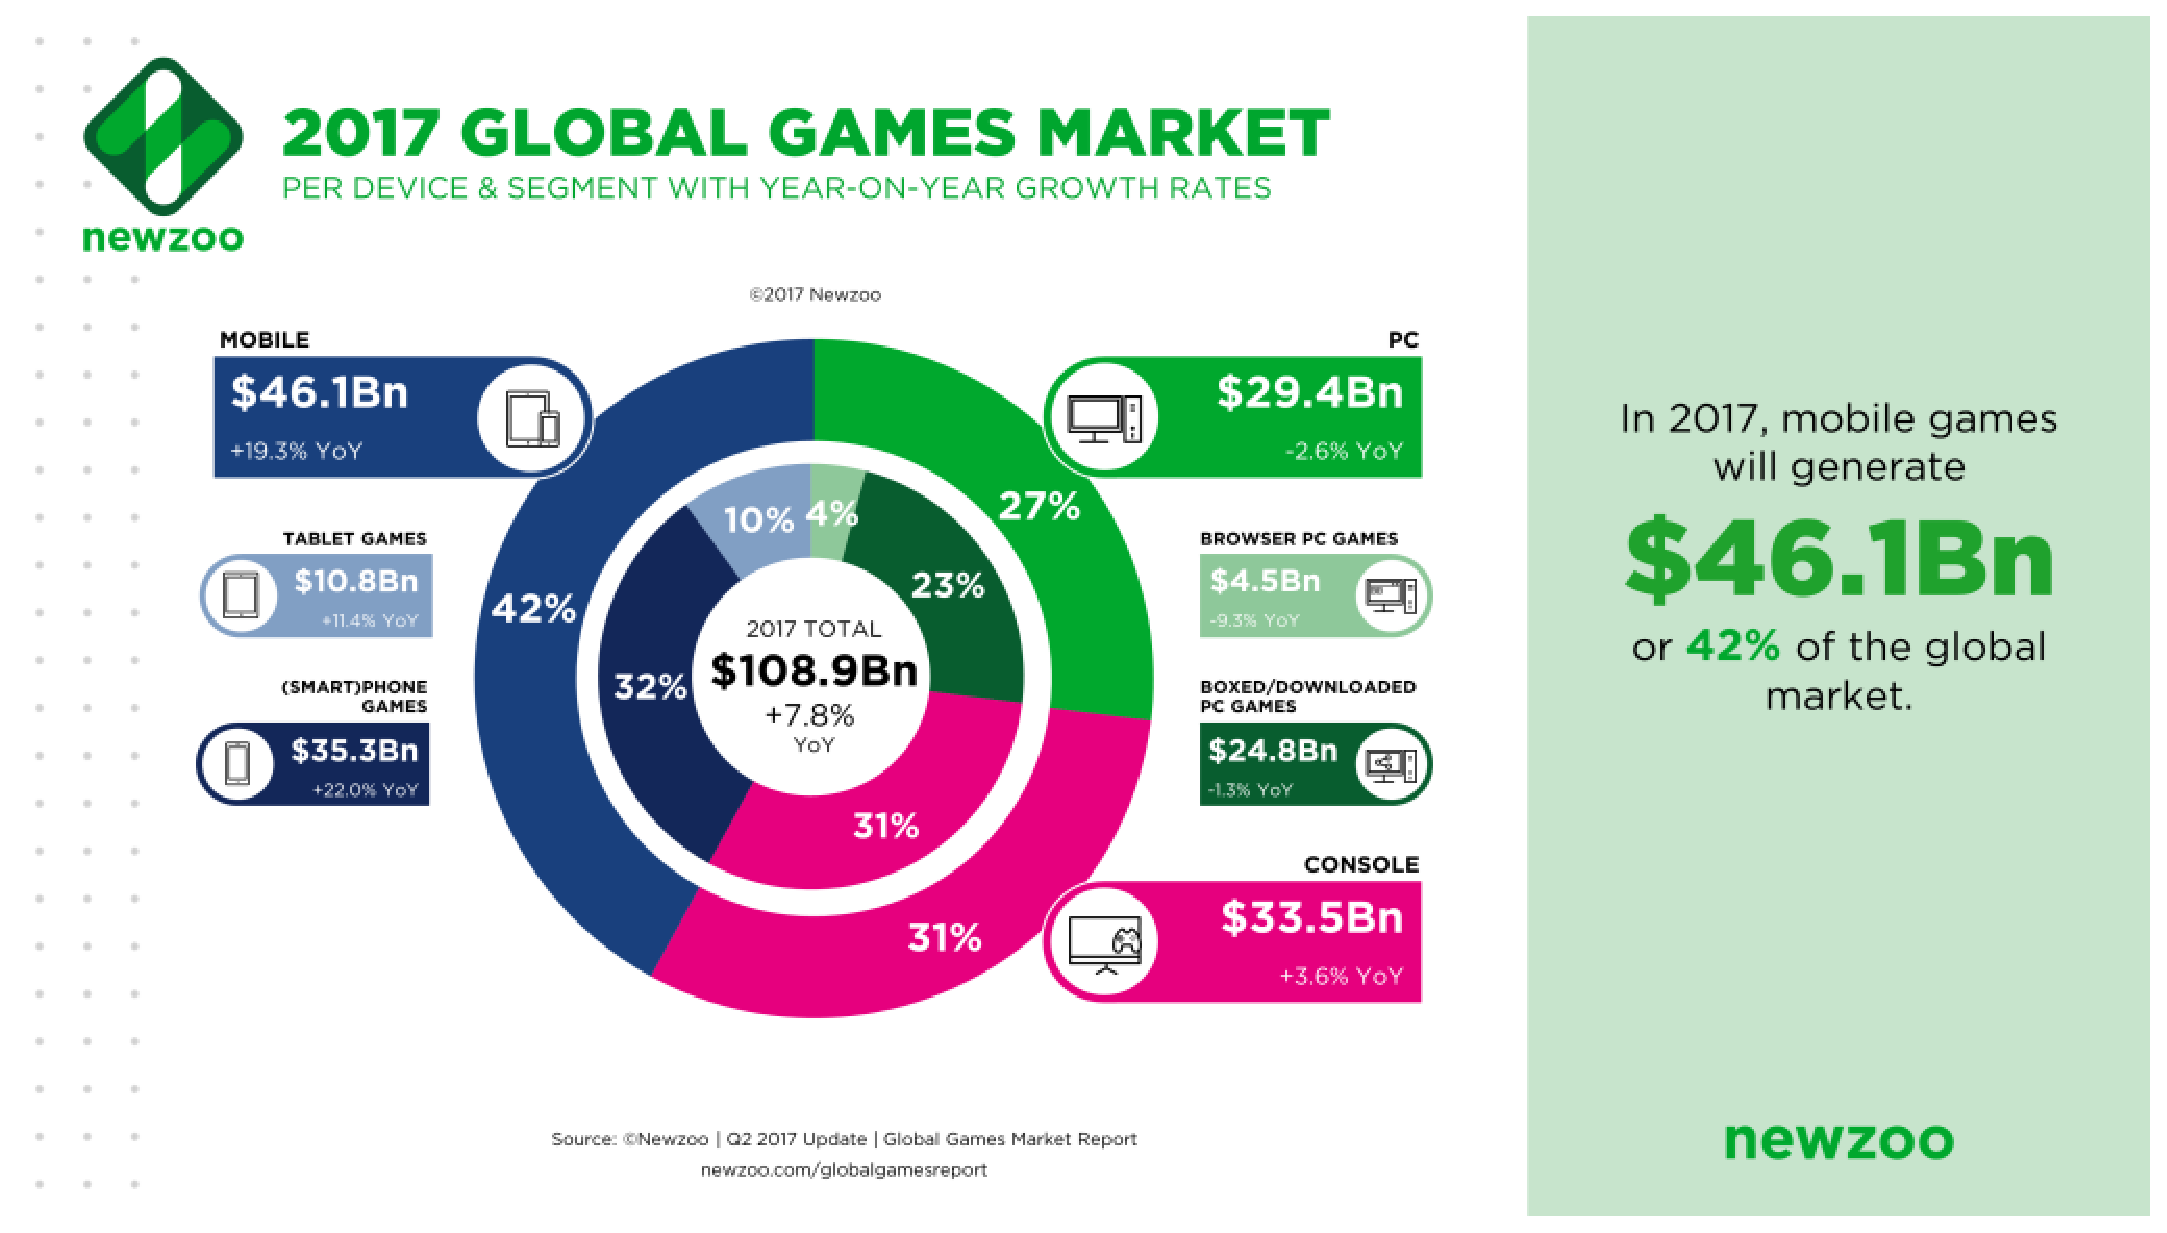
\includegraphics[width=\textwidth]{03MarcoTeorico/imageR/newzooIndMun}
			 	\caption{Mercado global de juegos por dispositivo y segmento con tasas de crecimiento interanual al año 2017.[Imagen](2017). Recuperado de: https://newzoo.com/resources/}
			 	\label{fig:newzooIndMun}
			 \end{figure}	
		 
		 Sabiendo lo anterior podemos ver la conveniencia que existe de realizar un videojuego dentro de los dispositivos móviles.
			 
			 
\subsection{Estudio de mercado en México}

Históricamente, México ha sido el país numero uno en el consumo de videojuegos en Latinoamérica como se ve en la imagen \ref{fig:mexicoUno}. Esto se debe a su cercanía con los Estados Unidos. Esto genera que se de una transmisión cultural y de tecnología casi inmediata. La industria de los videojuegos en México es cosa seria. 
\\[1pt] 
	\begin{figure}
	\centering
	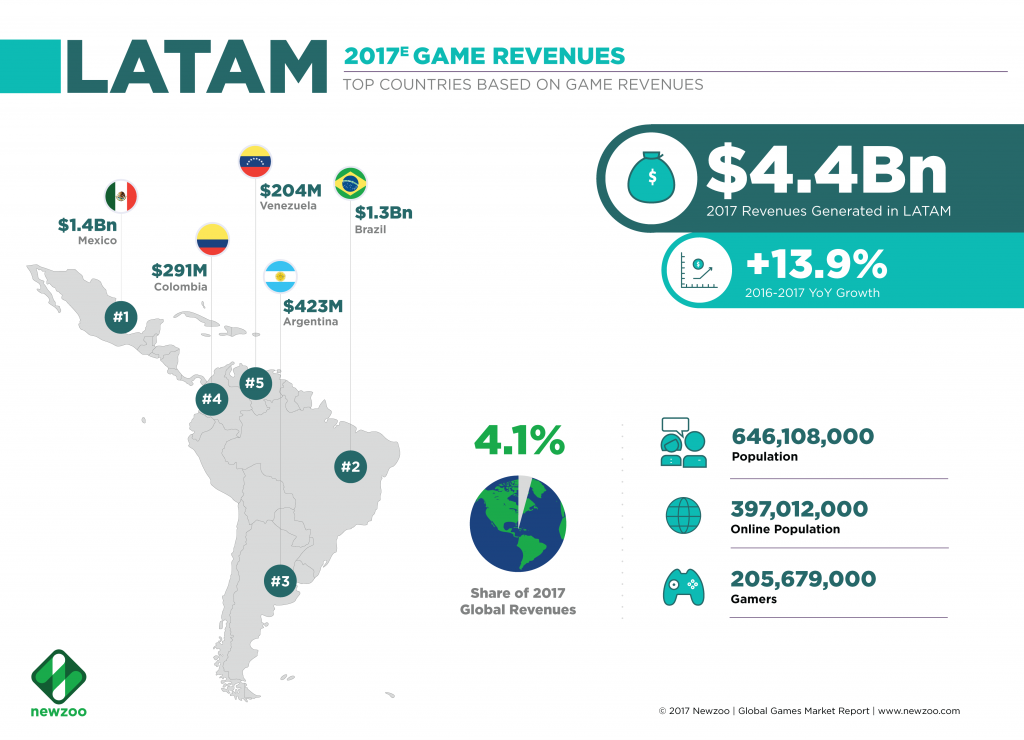
\includegraphics[width=\textwidth]{03MarcoTeorico/imageR/mexicoUno}
	\caption{Ingresos del juego en latinoamérica al año 2017.[Imagen](2017). Recuperado de: https://newzoo.com/resources/}
	\label{fig:mexicoUno}
	\end{figure}

Mientras que la economía nacional este mercado de entretenimiento pronostica un crecimiento anual de 8.4\% para 2017, es decir, casi cuatro veces lo que creció el Producto Interno Bruto (PIB) hace un año y lo que avanzaría al cierre del periodo en curso. De acuerdo con el estudio “Jugar no es cosa de niños: Dimensionamiento del Mercado de Videojuegos en México 1Q17” como se muestra en la imagen \ref{merVidMex}, elaborado por The Competitive Intelligence Unit (The CIU), este mercado tuvo ingresos por más de 22,852 millones pesos (mdp) en 2016, esto es, 13.3\% más con respecto al año anterior, con un número de usuarios de más de 65 millones \cite{vid03}. Y como lo analizamos en la industria mundial, también veremos los videojuegos en los dispositivos móviles.
\\[1pt] 
\begin{figure}
	\centering
	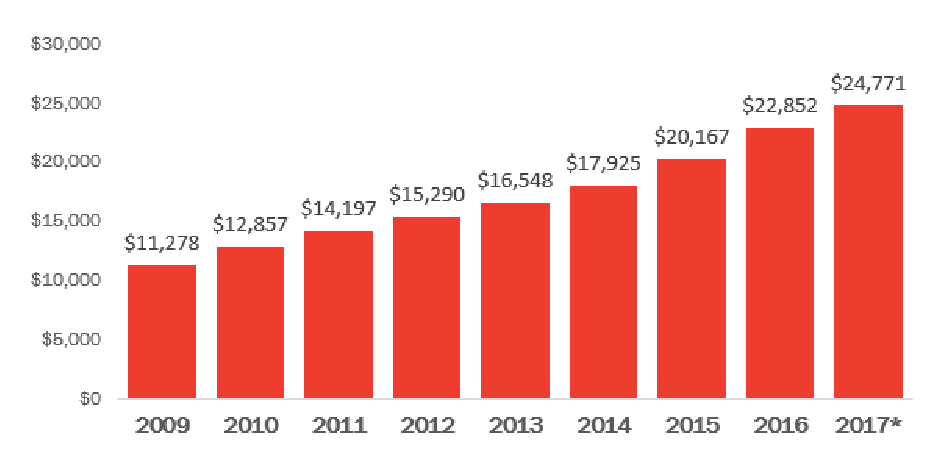
\includegraphics[width=0.5\textwidth]{03MarcoTeorico/imageR/merVidMex}
	\caption{Valor del mercado de videojuegos (Millones de pesos) elaborado por The Competitive Intelligence Unit (The CIU)[Imagen](2017). Recuperado de: http://the-ciu.net/nwsltr/152\_1Distro.html/}
	\label{fig:merVidMex}
\end{figure}

El teléfono móvil es el medio que ha mostrado mayor dinamismo en los videojuegos. Existen más de 90 millones de teléfonos inteligentes en uso dentro del país, lo que da acceso potencial a estas personas a miles de aplicaciones gratuitas y de paga existentes en el mercado. De esta manera, 66\% de los jugadores reportaron que utilizan su Smartphone, representando 39 millones de usuarios como se ve en la imagen \ref{fig:dispVid}. Y comprobamos el éxito potencial de los videojuegos en esta plataforma. Ahora veremos la frecuencia de juego que tienen las personas. 
\\[1pt] 	

\begin{figure}
	\centering
	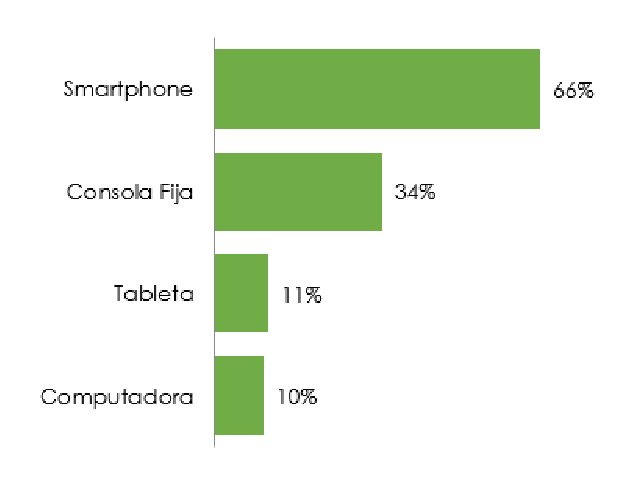
\includegraphics[width=0.5\textwidth]{03MarcoTeorico/imageR/dispVid}
	\caption{Grafica de dispositivos de acceso a videojuegos elaborado por The Competitive Intelligence Unit (The CIU)[Imagen](2017). Recuperado de: http://the-ciu.net/nwsltr/152\_1Distro.html/}
	\label{fig:dispVid}
\end{figure}

 El estudio revela que 63.7\% de los encuestados se asume como un usuario frecuente, que juega entre 1 y 3-4 veces a la semana; aunque de ese porcentaje el 40\% se asegura que juega entre una y dos veces por semana. Mientras que los ocasionales representan la parte menor con 5.4\%. De los llamado intensivos, por su parte, el 31.5\% juega diario o 5-6 veces a la semana como se ve en la imagen \ref{fig:frecJue}.
\\[1pt] 

\begin{figure}
	\centering
	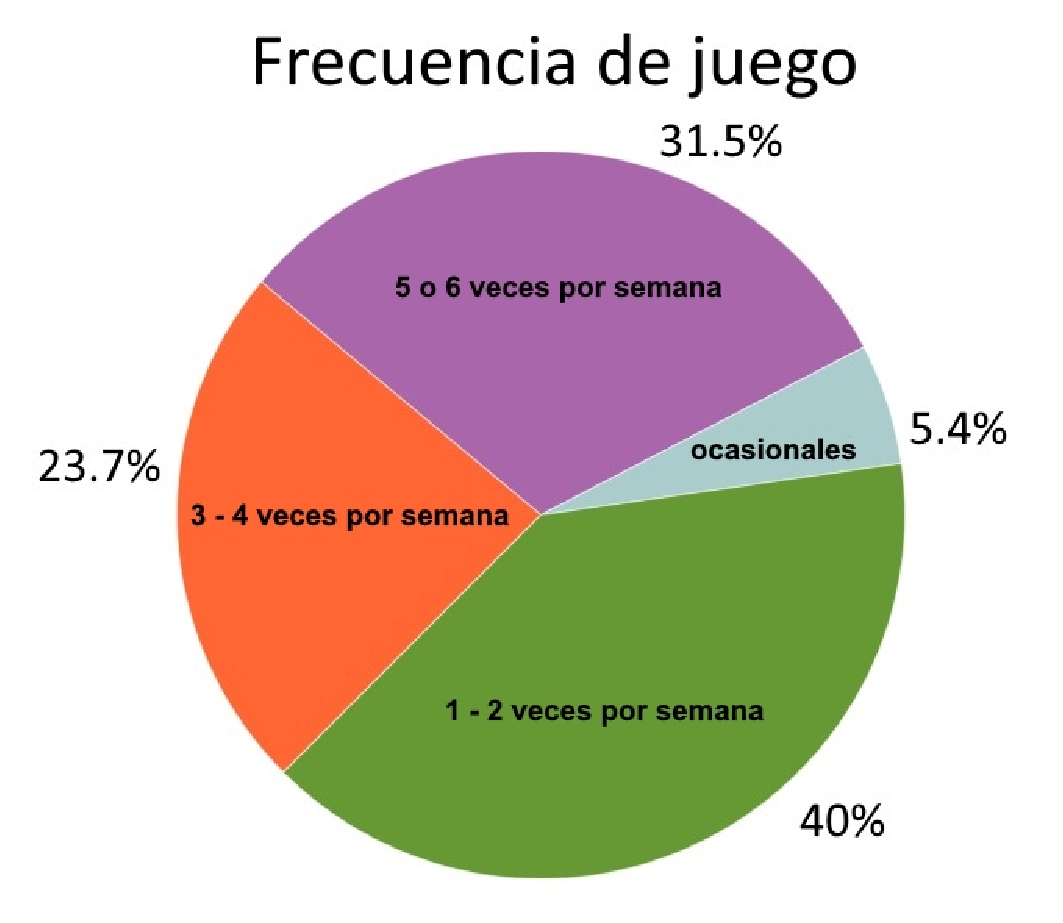
\includegraphics[width=0.5\textwidth]{03MarcoTeorico/imageR/frecJue}
	\caption{Grafica elaborada por encuesta de frecuencia de juego elaborado por The Competitive Intelligence Unit (The CIU)}
	\label{fig:frecJue}
\end{figure}

Así podemos concluir que en verdad México tiene mucha actividad dentro del consumo de videojuegos y convenientemente en una plataforma móvil.

\subsection{Industria en México}

La industria en México se refiere al desarrollo de videojuegos que existe dentro del país y no del consumo. La industria de producción de videojuegos en México se encuentra actualmente en una fase de desarrollo, debido a la persistente falta de oportunidades para desarrollarse en este tipo de actividad bajo un esquema corporativo o empresarial. Lo anterior se ve reflejado en la distribución del tipo de empleo de los desarrolladores nacionales, puesto que existe una alta proporción de empleados dedicados a la creación de videojuegos bajo un esquema independiente, son pocos casos los que llegan a consolidar su creación en una empresa con generación de empleos e ingresos en el largo plazo.
\\[1pt]

En México, la mayoría de empresas son micropymes, y no existe información abierta sobre su facturación o cuantas de ellas todavía no facturan. Muchas de estas pequeñas empresas recurren a soluciones como el crowndfounding mediante plataformas como Kickstarter para financiar su proyecto y buscan mentoring en las comunidades de desarrolladores cercanas\cite{vid05}. De acuerdo a estudios recientes, 40\% de los desarrolladores de videojuegos en México trabajan de modo independiente, mientras que únicamente 10\% de los desarrolladores han consolidado su propio negocio. Esto demuestra que una gran proporción de esta mano de obra se encuentra deslindada de grandes corporativos. En el caso de nuestro país como se ve en la imagen \ref{fig:desVj}, 6 de cada 10 desarrolladores dedican su actividad al desarrollo en smartphones y 32\% en tabletas, mientras que únicamente 26\% se especializan en el desarrollo de juegos en consolas fijas, respondiendo a una demanda de 40.7 millones de mexicanos que utilizan sus smartphones como principal dispositivo de juego \cite{vid04}.
\\[1pt]
\begin{figure}
	\centering
	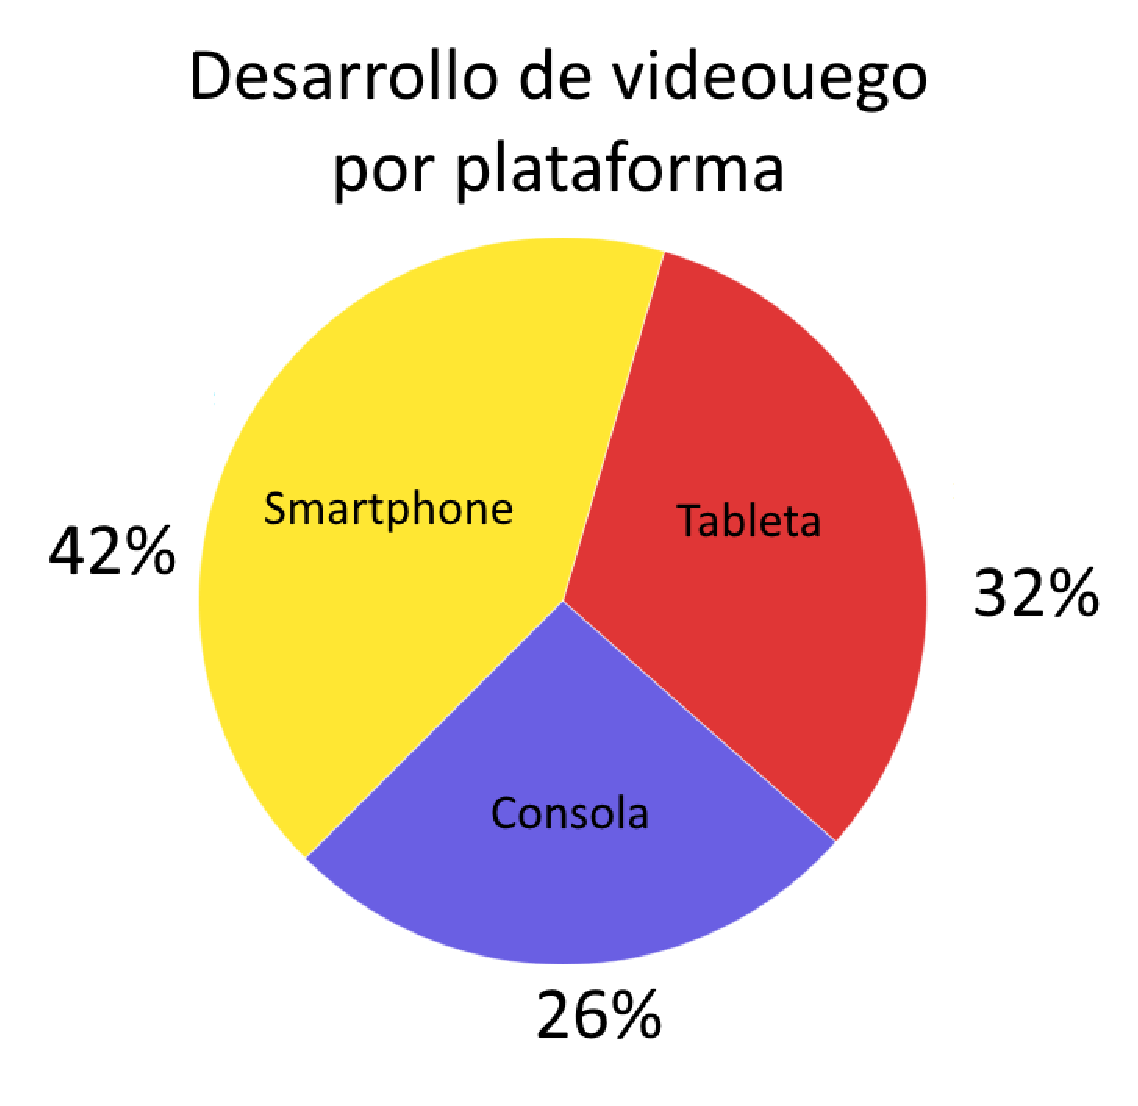
\includegraphics[width=0.3\textwidth]{03MarcoTeorico/imageR/desVj}
	\caption{Grafica de desarrollo de videojuego por plataforma en México realizada por encuesta de Competitive Intelligence Unit (The CIU).}
	\label{fig:desVj}
\end{figure}

Aquí una lista de estudios activos en México actualmente:
\begin{itemize}
	\item Larva Game Studios
	\item Kaxan Games
	\item Xibalba Studios
	\item Estudios Maquina Voladora
	\item Slang Studio
	\item Golden Pie Studio
	\item Kokonut Studio
	\item Phyne Games
	\item Playful Studios
	\item Squad Games
	\item Washa Washa
	\item Hollow Games
	\item HyperBeard Games
	
\end{itemize}

	\section{Desarrollo de videojuegos.}\label{DesVideojuego}
En esta sección se habla sobre el proceso de desarrollo del videojuego, hablando sobre los pasos que lleva el proceso de desarrollo; para despues describir las metodologias de desarrollo que se emplean, algunas de las metodologías descritas en este apartado son originarias del desarrollo de software convencional pero son adaptadas al desarrollo de software por algunos estudios independientes, es importante mencionar que muchas de las metodologias de desarrollo de videojuegos son propiedad de las empresas que las utilizan y por lo tanto no son de caracter público por lo que no pudieron ser incluidas en este trabajo terminal; para finalizar esta sección se habla sobre el software empleado en el desarrollo de videojuegos, entrandose en el motor de juego, el cual se define y se explica a grandez razgos su arquitectura.
	\subsection{Linea de producción de un videojuego.}\label{Pipelinevideojuego}
	Una linea de producción son los pasos o fases logicos y secuenciales requeridos para obtener un producto. Los pasos que componen la linea de producción dependen del producto que se va a fabricar y de la empresa fabricante. 
	\\
	\par	
	Existe una discrepacia en cuanto a que elementos tiene la linea de producción de un videojuego, siendo la representación más común la planteada por la revista ING, esta linea consiste en tres etapas\cite{Ref_Desarrollo}:
	\begin{itemize}
		\item \textbf{Concepto:} Es la idea que de origen a todo el juego que se va a realizar. Esta puede ser una simple oración en la que se mencione el contexto del juego y su tematica o también puede ser un acuerdo de la compañia desarrolladora para hacer una secuela o una precuela de un videojuego ya existente\cite{Ref_Desarrollo}.
	%===============================		
		\item \textbf{Preproducción:} En esta etapa el equipo de producción redacta el documento de diseño del videojuego, define el argumento, los persoanjes y la jugabilidad. En esta etapa se determinan todas las limitantes tecnicas y creativas que va a tener el proyecto\cite{Ref_Desarrollo}.
	%===============================
		\item \textbf{Producción:} En esta etapa se desarrolla el juego: los artistas desarrollan todos los elementos visuales que se van a emplear, los programadores se encargan de implementar la logica del juego y la jugabilidad establecida en la estapa de preproducción, el equipo de audio se encarga de generar todos los elementos de audio que conlleva el videojuego\cite{Ref_Desarrollo}.
	%===============================
		\item \textbf{Postproducción:} En esta etapa el juego se considera casi terminado y es sometido a diferentes pruebas para medir su rendimiento y encontrar y solucionar todo tipo de errores. Tambien en esta etapa se intensifican las campañas de promosión para el juego\cite{Ref_Desarrollo}.
\end{itemize}	 

	\subsection{Metodologías de desarrollo de videojuegos.}\label{MetodoVideojuego}

En esta sección se define lo que es una metodologia de desarrollo de software, 
se mencionan tres metodologías de desarrollo de software que emplea la industria de los videojuegos
y al final se menciona una metodología de desarrollo propia del desarrollo de videojuegos.

\subsubsection{¿Qué es una metodología de desarrollo de software?}
Las metodologías de desarrollo de software son un conjunto de procedimientos, técnicas y ayudas a la documentación para el desarrollo de productos software\cite{Ref_metodologia}.	En palabras de Gacitúa: "Una Metodología impone un proceso de forma disciplinada sobre el desarrollo de software con el objetivo de hacerlo más predecible y eficiente. Una metodología define una representación que permite facilitar la manipulación de modelos, y la comunicación e intercambio de información entre todas las partes involucradas en la construcción de un sistema"\cite{Ref_Metod}. 

%======================================================		
			\subsubsection{Metodología en cascada}
La metodología de desarrollo en cascada o también conocida como modelo de vida lineal o básico,  fue propuesta por Royce en 1970 y a partir de entonces ha tenido diferentes modificaciones. Sigue una progresión lineal por lo que cualquier error que no se haya detectado con antelación afectara todas las fases que le sigan provocando una redefinición en el proyecto y por ende un aumento en los costos de producción del sistema \cite{Ref:CarCascada}.
Esta metodología se divide en las siguientes etapas:
\begin{itemize}
	\item \textbf{Análisis de los requisitos del software}: En esta etapa se recopilan los requisitos del sistema, se centra especialmente en toda aquella información que pueda resultar de utilidad en la etapa de diseño, tales como tipos de usuarios del sistema, reglas de negocio de la empresa, procesos, etc. En esta etapa se responde la pregunta de ¿Qué se hará? 
	\item \textbf{Diseño}: Esta etapa se caracteriza por definir todas aquellas características que le darán identidad al sistema, tales como la interfaz gráfica, la base de datos, etc. Las características anteriormente definidas se obtendrán de la etapa de análisis. En esta etapa se respondería la pregunta de ¿Cómo se hará? 
	\item \textbf{Codificación}: Terminada la etapa de diseño, lo siguiente es programar y crear todos los elementos necesarios para el funcionamiento del sistema. 
	\item \textbf{Prueba}: Finalizada la decodificación se debe de probar la calidad del sistema. En este punto es importante resaltar que la pruebas no solo abarcan que se confirme que el sistema funcione, sino que también verifica que los usuarios puedan aprender a utilizarlo con facilidad, entre otros aspectos como la seguridad de la información y los tiempos de respuesta del sistema.
	\item \textbf{Mantenimiento}: En esta última etapa se realizarán modificaciones al sistema, sin que esto necesariamente signifique que estos cambios se deban a errores de programación, puesto que esta etapa también abarca agregar nueva funcionalidad al sistema o, en caso de que trabaje con protocolos de estándar internacional, actualizar sus protocolos \cite{Ref:CarCascada}. 
\end{itemize}
Algunos de los inconvenientes que presenta son:
\begin{itemize}
	\item No refleja el proceso de desarrollo real.
	\item Tiempos largos de desarrollo.
	\item Poca comunicación con el cliente.
	\item Revisiones de proyecto de gran complejidad.
\end{itemize}

%================================================
	\subsubsection{Metodología en Scrum}
Desarrollada por Ikujiro Nonaka e Hirotaka Takeuchi a principios de los 80’s, Esta metodología le debe su nombre a la formación scrum de los jugadores de ruby. Scrum es una metodología eficaz para proyectos con requisitos inestables que demandan flexibilidad y rapidez, esto principalmente a su naturaleza iterativa e incremental \cite{Ref_DefScrum}.  
\\
\par
Scrum parte de la visión general que se desea que producto alcance; a partir de esta visión se inicia la división del proyecto en diferentes módulos Scrum implementa una jerarquía entre los módulos en donde los módulos de mayor jerarquía son los que se desarrollaran al inicio del proyecto o durante las primeras iteraciones (sprint). Cada sprint tendrá una duración de hasta seis semanas a lo máximo \cite{Ref_ScrumRef}. 
\\
\par
Durante el proceso de desarrollo del sprint, el equipo tendrá reuniones diarias en donde se definirán metas diarias para lograr completar el objetivo del sprint. Estas reuniones deberán de ser de corta duración (no más de quince minutos) y recibirán el nombre de scrum diario. Al final de cada sprint, el equipo contará con un módulo funcional que el cliente podrá utilizar sin que el sistema este completado.
\\
\par
Cada sprint se compone de las siguientes fases:
\begin{itemize}
	\item Concepto: se define a grandes rasgos las características del producto y se asigna a un equipo para desarrollarlo.
	\item Especulación: Con la información del concepto se delimita el producto, siendo las principales limitantes los tiempos y los costes. Esta es la fase más larga del sprint. En esta etapa se desarrolla basándose en la funcionalidad esperada por el concepto.
	\item Exploración: El producto desarrollado se integra al proyecto.
	\item Revisión: Se revisa lo construido y se contrasta con los objetivos deseados.
	\item Cierre: Se entrega el producto en la fecha programada, esta etapa no siempre significa el fin del proyecto; en ocasiones marca el inicio de la etapa de mantenimiento \cite{Ref_ScrumGuia}. 
\end{itemize}
Uno de los principales componentes de la metodología scrum son los roles, es decir el papel que cada integrante del equipo desempeñara durante el proceso de desarrollo. Los roles se dividen en dos grupos:
\begin{itemize}
	\item Cerdos : Son los que están comprometidos con el proyecto y el proceso de Scrum.
		\begin{itemize}
			\item Product owner: Es el jefe del proyecto y por lo tanto es quien toma las decisiones. Esta persona es quien conoce más del proyecto y las necesidades del cliente. Es el puente de comunicación entre el cliente y el resto del equipo. 
			\item Scrum Master: Se encarga de monitorear que la metodología y el modelo funcionen. Es quien toma las decisiones necesarias para eliminar cualquier inconveniente que pueda surgir durante el proceso de desarrollo. 
			\item Equipo de desarrollo: Estas personas reciben el objetivo a cumplir del Product owner y cuentan con la capacidad de tomar las decisiones necesarias para alcanzar dicho objetivo.
		\end{itemize}
	\item Gallinas: Personas que no participan de manera directa en el desarrollo, sin embargo, su retroalimentación da pie a la planeación de los sprints.
		\begin{itemize}
			\item Usuarios: Son quienes utilizaran el producto.
			\item Stakeholders: Son quienes el proyecto les aportara algún beneficio. Participan en las revisiones del sprint.
			\item Manager: Toma las decisiones finales. Participa en la selección de objetivos y en la toma de requerimientos\cite{Ref_ScrumRef}.
		\end{itemize}
\end{itemize}

%=============================
\subsubsection{Metodología de Programación extrema}
La metodología de programación extrema o metodología XP(por sus siglas en inglés) fue desarrollada por Kent Beck en 1999 basándose en la simplicidad, la comunicación y le retroalimentación de código. Es una metodología de desarrollo ágil y adaptativa, soporta cambios de requerimientos sobre la marcha. Su principal objetivo es aumentar la productividad y minimizar los procesos burocráticos, por lo que el software funcional tiene mayor importancia que la documentación\cite{Ref_XP}.
\\
\par
  XP se fundamenta en doce principios que se agrupan en cuatro categorías. A continuación, se hará mención de estos principios:
\begin{itemize}
	\item Retroalimentación:
		\begin{itemize}
			\item Principio de pruebas: Se define la el periodo de pruebas de funcionalidad del software a partir de sus entradas y salidas como si se tratara de una caja negra.
Planificación: El cliente o su representante definirá sus necesidades y sobre ellas se redactará un documento, el cual servirá para establecer los tiempos de entregas y de pruebas del producto.
			\item Cliente in-situ: El cliente o su representante se integrarán al equipo de trabajo con la finalidad de que participen en la planeación de tareas y en la definición de la funcionalidad del sistema. Esta estrategia se implementa para minimizar los tiempos de inactividad entre reuniones y disminuye la documentación a redactar.
			\item Pair-programming: Se asignan parejas de programadores para desarrollar el producto. Esto generará mejores resultados en menores costos.
		\end{itemize}
	\item Proceso continuo en lugar de por bloques
		\begin{itemize}
			\item Integración continua: Se implementan progresivamente las nuevas características del software. Esta integración no se hace de manera modular ni planeada.
			\item Refactorización: La eliminación de código duplicado o ineficiente les permite a los programadores mejorar sus propuestas en cada entregable.
			\item Entregas pequeñas: Los tiempos de entregas son cortos y permiten la evaluación del sistema bajo escenarios reales.
		\end{itemize}
	\item Entendimiento compartido
		\begin{itemize}
			\item Diseño simple: El programa que se utiliza en los entregables es aquel que tenga la mayor simplicidad y cubra las necesidades del cliente.
			\item Metáfora: expresa la visión evolutiva del proyecto y define los objetivos del sistema mediante una historia.
			\item Propiedad colectiva del código: Todos los programadores son dueños del programa y de las responsabilidades del programa. Un programa con muchos programadores trabajando en él es menos propenso a errores. 
			\item Estándar de programación: Se define la estructura que tendrá el programa a la hora de ser escrito, esto para dar la impresión de que una sola persona trabajo en él.
		\end{itemize}
	\item Bienestar del programador
		\begin{itemize}
			\item Semana de 40 horas: Se minimizan las jornadas de trabajo excesivas para grantizar el mejor desempeño del equipo\cite{Ref_XPPrincipios}.
		\end{itemize}
\end{itemize}
Tal como se puede observar XP, es una metodología fuertemente orientada hacia los miembros del equipo, su bienestar, la interacción entre ellos y en su aprendizaje.

%==========================================
\subsubsection{Metodología Huddle}
Huddle es una metodología creada por el Instituto de Ingeniería y Tecnología de Universidad Autónoma de Ciudad Juárez. Huddle recibe su nombre por las reuniones que se realizan en el futbol americano antes de cada jugada. Su funcionalidad se basa en la metodología Scrum, con la diferencia de que está orientada en el desarrollo de videojuegos.  De naturaleza ágil, resulta óptimo para equipos multidisciplinarios de 5 a 10 personas; es iterativa, incremental y evolutiva \cite{Ref_Huddle}.
\\
\par
Huddle se divide en tres etapas: 
	\begin{itemize}
		\item Preproducción: Consiste en la planeación del juego. En esta etapa se redactará el documento de diseño; este documento contendrá la idea general del juego, su escritura deberá de ser tal que todos los miembros del equipo pueden entenderlo y darse una idea de cómo será el juego una vez que se haya terminado. En esta etapa se definirá el argumento del juego, sus personajes, el género del juego, sus mecánicas, la música, los efectos de sonido, los efectos especiales y su funcionalidad. Huddle proporciona plantilla para realizar este documento, dejando la posibilidad de modificarlo según el equipo considere oportuno.
		\item Producción: Es la etapa más larga y de mayor importancia. Su organización se basa totalmente en la organización iterativa e incremental de Scrum; es decir se harán reuniones diarias en donde se discutirán los objetivos de la iteración. Antes de finalizar cada Sprint, el módulo se someterá a diferentes pruebas para garantizar su funcionalidad. Cuando un Sprint finaliza, se realiza una reunión en la que los elementos del quipo discuten las decisiones tomadas y analizan cuales fueron las decisiones y acciones más eficientes para retomarlas y desechar aquellas que atrasen al proyecto. Al finalizar esta etapa el equipo contará con las versiones alfa y beta del juego. 
		\item Postmorten: En esta etapa se discuten todos los puntos positivos y negativos del proyecto. En esta evaluación se redactará un documento que permita a futuros proyectos efectuar planes de acción más efectivos\cite{Ref_Huddle}.
	\end{itemize}

	\subsection{Software para el desarrollo de videojuegos.}\label{SoftVideojue}
En este apartado se habla del software que comúnmente se emplea para el desarrollo de videojuegos, empezando por el motor de juego, la definición del motor de juego, la arquitectura del motor de juego, los motores de juego más usados en el mercados; para finalizar con una lista del software auxiliar que se usa para generar lo elementos visuales y auditivos que componen al juego.

%==========================================
 
\subsubsection{Motor de juego.}
El motor de juego, también conocido como Game Engine, parte del concepto de reutilización; es decir, es posible generar juegos a partir de un código base y común mediante una separación adecuada de los componentes fundamentales, tal como visualización de gráficos, control de colisiones, físicas, entrada de datos etc \cite{Ref:MutorGraf}; esto permite a quienes trabajen en un juego puedan centrarse en todos aquellos detalles que hacen al juego único.

%==========================================

\subsubsection{Arquitectura del motor}
Los motores de juego se basan en una arquitectura estructurada a capas. Por lo que las capas de nivel superior dependen directamente de las de nivel inferior \cite{Ref:ArquMotor} 
 A continuacion se mencionaran las capas que componen al motor de juego junto a una breve descripción de la capas.
 
 \begin{itemize}
 	\item \textbf{Hardware:} esta capas e relaciona con la plataforma sobre la que se ejecutará el juego. Existen motores gráficos orientados hacia una sola plataforma (dispositivos móviles, consolas caseras, computadoras o consolas portátiles, etc.) y existe motores multiplataforma que permiten el desarrollo simultaneo de un juego para diferentes plataformas (cross-platform) \cite{Ref:ArquMotor}.
 	\item \textbf{Drivers:} Esta capa garantiza la correcta gestión de determinados dispositivos (tarjeta grafica, tarjeta de sonido, etc.) haciendo uso de software de bajo nivel \cite{Ref:ArquMotor}. 
 	\item \textbf{Sistema Operativo:} Esta capa garantiza la comunicación de los procesos que se ejecutan en el sistema operativos y los recursos de la plataforma asociada con el juego \cite{Ref:ArquMotor}.
 	\item {Kits de de desarrollo de software y middleware:} Un Kit de de desarrollo de software(SDK, por sus siglas en inglés) son todas aquella herramientas que le permiten al programador desarrollar aplicaciones informaticas para una plataforma determinada \cite{ref:SDK}. Mientras que un middleware es software que se sitúa entre un sistema operativo y las aplicaciones que se ejecutan en él. Básicamente, funciona como una capa de traducción oculta para permitir la comunicación y la administración de datos en aplicaciones distribuidas \cite{Ref:middleware}. 
 	\item \textbf{Capa independiente de la plataforma:} Esta capa aísla las capas dependientes de la plataforma para la que se va a desarrollar el juego, de las capas superiores que son estándares e independientes de la plataforma \cite{Ref:ArquMotor}. 
 	\item \textbf{Subsistemas principales:} Esta capa esta compuesta sub sistemas que vinculan a todas aquellas utilidades o bibliotecas de utilidades que dan soporte al motor de juegos. Tal como:
 	\begin{itemize}
 		\item Biblioteca matemática.
 		\item Estructuras de datos y algoritmos.
 		\item Gestión de memoria.
 		\item Depuración y logging \cite{Ref:ArquMotor}.
 	\end{itemize}
 	\item \textbf{Gestor de recursos:} Esta capa es responsable de generar una interfaz de comunicación unificada para acceder a las distintas entidades de software que componen el motor de juego, como por ejemplo las escenas, los sonidos o los objetos de juego \cite{Ref:ArquMotor}.
 	\item \textbf{Motor de rendering:} Renderizado (render en inglés) es un término usado en computacion para referirse al proceso de generar una imagen foto realista desde un modelo 3D \cite{Ref:Render}. Esta capa tiene una gran importancia, debido a la naturaleza gráfica del videojuego. El enfoque más utilizado para implementar esta capa es utilizando una arquitectura multi-capa\cite{Ref:ArquMotor}.
 	\item \textbf{Herramientas de depuración:} Esta capa se encarga de depurar y optimizar el motor de juego para obtener un mejor rendimiento\cite{Ref:ArquMotor}.
 	\item \textbf{Motor de Física:} Esta capa se encarga de gestionar la detección de colisiones, su determinación y la posterior respuesta que tendrá el juego ante dicha colisión.
 	\item \textbf{Interfaces de usuario:} Esta capa tiene como objetivo ofrecer una abstracción de las interacciones del usuario con el juego y de tratar todos los eventos de salida, es decir la retroalimentación que el juego le da al usuario\cite{Ref:ArquMotor}.
 	\item \textbf{Networking y multijugador:} Esta capa permite que el juego sea capaz de soportar diferentes jugadores de manera simultanea, ya sea que se encuentren de manera local (es decir en una misma plataforma sin conexión a internet) o de manera online (haciendo uso del internet)\cite{Ref:ArquMotor}.
 	\item \textbf{Subsistema de juego:} Esta capa permite la creación de las mecánicas de juegos; es decir es capa soporta la implementación de un lenguaje de programación, comúnmente de alto nivel, para definir el comportamiento de todos aquellos elementos que componen el juego, como enemigos, cámaras, obstáculos, etc \cite{Ref:ArquMotor}.
 	\item Audio: Esta capa proporciona al moto la capacidad de utilizar archivos de audio para garantizar una mejor experiencia al usuario\cite{Ref:ArquMotor}.
 	\item \textbf{Subsistemas específicos de juego:} En esta capa se implementan todos aquellos módulos que proporcionen una identidad al sistema y por lo tanto son únicos\cite{Ref:ArquMotor}.
 \end{itemize}	
 
%========================================== 
 
 \subsubsection{Motores gráficos existentes en el mercado.}
En este apartado se mencionaran los principales motores de juego que existen en la industria, de igual manera se hará mención de sus principales características.

	\begin{itemize}
			%=====================================
		\item \textbf{Unity3D:} Actualmente Unity es el motor grafico más utilizado en la industria. 
			\begin{itemize}
				\item \textbf{Sistema operativo:} Microsoft ver 10,8, 7(solo 64 bits); MacOs ver X 10.9 en adelante.
				\item \textbf{CPU:} Soporte para el conjunto de instrucciones SSE2.
				\item \textbf{GPU:} Tarjeta gráfica con DX9 (modelo de shader 3.0) o DX11 con capacidades de funciones de nivel 9.3.
				\item \textbf{Memoria RAM:} Depende de la complejidad del proyecto.
				\item \textbf{Desarrollo para plataforma:} Cross-platform.
				\item \textbf{Orientado a 2D/3D:} 2D y 3D.
				\item \textbf{Lenguaje de programación que soporta:} $\sharp C$, javaScript, Boo.
				\item \textbf{Tipo de Licencia:} Maneja tres tipos de licencia, dos de pago y uno gratuito. \cite{Ref:Unity} 
			\end{itemize}		
		%=====================================
		\item \textbf{UnrealEngine:} Considerado por algunas revistas especialistas en videojuegos como el motor de juego más potente. 
			\begin{itemize}
				\item \textbf{Sistema operativo:} Microsoft ver 10,8, 7(solo 64 bits); macOS 10.13 High Sierra y Ubuntu 15.04.
				\item \textbf{CPU:} SQuad-core Intel or AMD, 2.5 GHz or faster (Para Windows), Quad-core Intel, 2.5 GHz or faster(Para Mac y linux).
				\item \textbf{Tarjeta de vídeo:} DirectX 11 compatible graphics card (Para Windows), Metal 1.2 Compatible Graphics Card(Para Mac) y NVIDIA GeForce 470 GTX or higher with latest NVIDIA binary drivers(Linux). 
				\item \textbf{Memoria RAM:} 8GB (Microsoft y Mac) y 16GB (Linux).
				\item \textbf{Desarrollo para plataforma:} Cross-platform.
				\item \textbf{Orientado a 2D/3D:} 2D y 3D.
				\item \textbf{Lenguaje de programación que soporta:} C++.
				\item \textbf{Tipo de Licencia:} licencia de pago pero se debe de pagar el 5 por ciento de las regalias cuando el juego sea publicado. \cite{Ref:Unreal}
			\end{itemize}
		%=====================================
		\item \textbf{CryEngine:} Considerado por algunas revistas especialistas en videojuegos como el motor de juego más potente. 
			\begin{itemize}
				\item \textbf{Sistema operativo:} Microsoft ver 10,8, 7(solo 64 bits y 32 bits).
				\item \textbf{CPU:} Intel Dual-Core min 2GHz (Core 2 Duo and above) o AMD Dual-Core min 2GHz (Phenom II X2 and above).
				\item \textbf{Tarjeta de vídeo:} NVIDIA GeForce 450 series o AMD Radeon HD 5750 series or higher (minimum 1 GB dedicated VRAM GDDR5). 
				\item \textbf{Memoria RAM:} 4GB.
				\item \textbf{Desarrollo para plataforma:} Cross-platform.
				\item \textbf{Orientado a 2D/3D:} 2D y 3D.
				\item \textbf{Lenguaje de programación que soporta:} C++, $\sharp C$ y Lua.
				\item \textbf{Tipo de Licencia:} Licencia gratuita pero ofrece planes de pago para capacitación. \cite{Ref:CryEngine}
			\end{itemize}						
		
	\end{itemize}
	
	%===================================
	\subsubsection{Software auxiliar}
	Además de los motores gráficos el proceso de desarrollo de videojuegos necesita diferentes herramientas auxiliares para la creación de todos aquellos elementos que se necesiten poner dentro del juego, sea personajes, música, fondos, efectos de sonido, etc. A continuación, se mostrará una lista de aplicaciones y páginas web que fungen como herramientas auxiliares en el desarrollo de videojuegos:
	
	\begin{itemize}
	%===================================================
		\item Creación de Sprites (Solo juegos 2D) o texturas.
			\begin{itemize}
	%===================================================
				\item Adobe Photoshop.
					\begin{itemize}
						\item Descripción: Aplicación de diseño y tratamiento de imágenes. Con esta aplicación se pueden crear ilustraciones e imágenes 3d. Su capacidad de manejo de imágenes secuenciales la hacen de gran ayuda en la generación de imágenes de bloques de animación para los sprites de juegos 2D, así como su compatibilidad con Adobe Ilustrator facilitan la vectorización de sprites.
						\item Requerimientos mínimos en Windows:
						\begin{itemize}
							\item Procesador Intel Core 2 o AMD Athlon 64 processor de 2 GHz.
							\item Sistema operativo Microsoft Windows 7, Windows 8.1, o Windows 10.
							\item 2 GB de RAM.
							\item Espacio de 2.6 GB en el disco duro para instalcion en 32 bits; o 3.1 GB para sistemas de 64 bits.
							\item Pantalla de 1024 x 768 con 16-bit de color y 512 MB de VRAM [].
						\end{itemize}
					\end{itemize}
%===================================================					
				\item Adobe Ilustrator.
					\begin{itemize}
						\item Descripción: Esta aplicación de gráficos vectoriales permite crear logotipos, iconos, dibujos, tipografías e ilustraciones para ediciones impresas, la web, vídeos y dispositivos móviles. Su sistema de vectorización de imágenes permite crear sprites de mejor calidad.  Es una buena herramienta para la creación de botones o iconos para la GUI de juegos.
						\item Requerimientos mínimos en Windows:
							\begin{itemize}
								\item Procesador Intel Pentium 4 or AMD Athlon 64 processor
								\item Sistema operativo Microsoft Windows 7, Windows 8.1, o Windows 10
								\item 1 GB de RAM para 32 bits; 2 GB de RAM para 64 bit
								\item 2 GB libres en el disco duro.
								\item Pantalla de 1024 x 768, 1GB de VRAM.
							\end{itemize}

					\end{itemize}
%===================================================
				\item AutoDesk SketchBook.
					\begin{itemize}
						\item Descripción: Herramienta de diseño, más orientada hacia artistas que hacía diseñadores. Es una herramienta de gran utilidad en la creación de arte conceptual para el juego y el diseño de personajes. También posee una herramienta que permite la creación de imágenes secuenciales para bloques de animación. Tiene una total compatibilidad con Adobe Photoshop, por lo que se pueden exportar proyectos desde AutoDesk SketchBook sin el temor de perder detalles de diseño. Su principal ventaja es que se encuentra disponible para dispositivos móviles (Android e IOS) y computadoras (Windows y  MAC), cuenta con tres tipos de licencias: la gratuita (tiene funcionalidad limitada), la de pago (por un único pago se cuenta con varias herramientas de diseño) y la pro (Suscrición mensual que ofrece la total funcionalidad de la aplicación y permite utilizar toda funcionalidad  tanto en dispositivos móviles como en computadoras ).
						\item Requerimientos mínimos en Windows:
							\begin{itemize}
								\item Sistema operativo Windows 7 SP1 (32 bit, 64 bit), Windows 8/8.1 (32 bit, 64 bit), o Windows 10.
								\item Procesador de 1 GHz Intel o AMD CPU.
								\item 1GB de Memoria.
								\item 256 MB de tarjeta gráfica con soporte de OpenGL 2.0.

							\end{itemize}
					\end{itemize}
			\end{itemize}
%===================================================
		\item Modelos 3D y animación 3D.
			\begin{itemize}
				\item Blender.
					\begin{itemize}
						\item Descripción: Aplicación de modelado y animación 3D de licencia libre. Se encuentra disponible para Windows, Linux y macOS. Blender permite la exportación de modelos, paquetes de animación y escenarios enteros a motores gráficos como Unity3D.
						\item Requerimientos mínimos:
							\begin{itemize}
								\item CPU de 32-bit dual core 								\item 2Ghz  con soporte a SSE2.
								\item 2 GB de memoria RAM.
								\item Pantalla de 24 bits 1280 x 768.
								\item OpenGL 2.1 Compatible con gráficos y con 512 MB RAM.
							\end{itemize}
					\end{itemize}
%===================================================
				\item Maya.
					\begin{itemize}
						\item Descripción: Es un software de renderización, simulación, modelado y animación 3D. Maya ofrece un conjunto de herramientas integrado y potente, que puede usar para crear animaciones, entornos, gráficos de movimiento, realidad virtual y personajes. Se encuentra disponible para Windows, Linux y macOS.
						\item Requerimientos mínimos:
							\begin{itemize}
								\item Procesador de varios núcleos de 64 bits Intel o AMD con el conjunto de instrucciones SSE4.2.
								\item 8 GB de RAM.
								\item 4 GB de espacio libre en disco para la instalación.
							\end{itemize}
					\end{itemize}
			\end{itemize}
%===================================================
		\item Edición y creación de sonido.
			\begin{itemize}
				\item Ardour
					\begin{itemize}
						\item Descripción: Software que permite grabar, editar y mezclar audio. Su público objetivo son ingenieros de audio, compositores, músicos y editores se soundtracks. Se encuentra disponible para Mac, Windows y Linux. Posee soporte para pluings.
						\item Requerimientos mínimos para Linux:
						\begin{itemize}
							\item Cualquier procesador de 32 o 64 bits Intel.
							\item Cualquier distribucion de linux con un kernel más actual al 2.3 y libc version 2.25 
							\item 2GB de RAM.
							\item Espacio minimo de 350MB en el disco duro.

						\end{itemize}
					\end{itemize}
			\end{itemize}
\end{itemize}
	
	
	\section{Gamificación}
La gamificación es el uso de las mecánicas de juego en entornos ajenos al juego, según el término anglosajon definido por Sebastian Deterding (Diseñador/investigador del diseño de juego para el florecimiento humano) \cite{gameDef}. Es decir, que cualquier tema o asunto a tratar puede pasar por un proceso para convertirse en un juego. Y deben de cumplir con características específicas según el profesor Santiago Moll\cite{gameficacion}, estas son: mecánicas o reglas, dinámicas de juego, y componentes. También describe que clase de jugadores existen, el proceso que debe de llevar un tema a gamificar y la finalidad que debe cumplir. Todo esto se muestra a continuación.
\\[1pt]

\subsection{Característcas}
Las características a presentar son una guía para realizar un juego y no necesariamente se debe cumplir con todas y cada una de ellas. Sin embargo estas características ayudan en gran medida al entretenimiento del jugador. Recordemos que las características a presentar incluyen las mecánicas o reglas, dinámicas de juego y componentes.
\\[1pt]
 
\textbf{Mecánicas o reglas}
\\[1pt]
Son las normas de funcionamiento que permiten se adquiera un compromiso del jugador con el juego. Mantienen al jugador en constante actividad y le permite ver los límites que existen en el juego.
\\[1pt]

\begin{itemize}
	\item Colección: Logros y recompensas que consigue el jugador.
	\item Puntos: Para motivación y conteo de realizar una tarea por el jugador.
	\item Ranking: Clasificación o comparación entre jugadores.
	\item Nivel: Reflejan el progreso del jugador.
	\item Progresión: Consiste en completar el 100\% de la actividad encomendada al jugador.	
\end{itemize}

\textbf{Dinámicas de juego}
\\[1pt]
Motivan y despiertan el interés del jugador de realizar una actividad dentro del juego. Aunque no es necesario cumplir con este requisito para un juego son clave para mantener jugando a la persona.  

\begin{itemize}
	\item Recompensa: Premio por realizar alguna actividad en el juego.
	\item Competición: Deseo de estar en una determinada posición o grado en el juego entre los participantes.
	\item Cooperativismo: Otra forma de competir pero en un grupo de jugadores con un mismo fin o meta del juego.
	\item Solidaridad: Se fomenta la ayuda entre jugadores y debe ser de manera altruista.
\end{itemize}

\textbf{Componentes}
\\[1pt]
Los componentes se encargan de personalmente darle a cada jugador su estado en el juego. Así son identificados por los demás participantes fácilmente en las actividades que destacan o han realizado con exito. También cumplen con la parteen la que el jugador puede proyectarse dentro juego.
\begin{itemize}
	\item Logros: Visualizan el alcance del jugador de un objetivo del juego.
	\item Avatares: Representación gráfica del jugador.
	\item Medallas: Insignia o distintivo del jugador que ha ganado.
	\item Desbloqueo: Permiten avanzar en las actividades del juego gracias a actividades previas hechas por el jugador.
	\item Regalos: Un presente por la realización correcta de un reto por el jugador	.
\end{itemize}

\subsection{Tipos de jugadores}
Para saber que elementos debe llevar el juego a realizar debe conocerse los tipos de jugadores que existen. También se debe de saberse las motivaciones que los impulsan a seguir jugando. A continuación se muestran cuatro identificados.
\begin{itemize}
	\item Triunfador: Su finalidad es la consecución de logros y retos.
	\item Social: Le encanta interactuar y socializarse con el resto de compañeros.
	\item Explorador: Tiene tendencia a descubrir aquello desconocido.
	\item Competidor: Su finalidad es demostrar su superioridad frente a los demás.
\end{itemize}


\subsection{Proceso}
Ahora se seguirá los pasos para convertir un tema a un juego. Conociendo ya los elementos que disponemos y haber identificado al tipo de jugador que queremos, podemos convertir nuestro tema o actividad en un juego. 
\begin{itemize}
	\item Viabilidad: Determinar si el contenido que se quiere enseñar es jugable.
	\item Objetivos: Definir los objetivos del juego.
	\item Motivación: Valorar la predisposición y el perfil de jugadores.
	\item Implementación: Relación entre el juego y contenido a enseñar.
	\item Resultados: Evaluación de la actividad en el juego.
\end{itemize}


\subsection{Finalidad}
En cada juego se debe tener claro lo que quiere lograrse, es decir la finalidad del juego. Debe de determinarse que se desea lograr con el jugador.
\begin{itemize}
	\item Fidelización: Establecer un vínculo del contenido del juego con el jugador.
	\item Motivación: Crear una herramienta contra el aburrimiento del contenido a tratar.
	\item Optimización: Recompensar al jugador en aquellas tareas en las que no tiene previsto ningún incentivo.
\end{itemize}

	\section{Cultura.}\label{cultura}
	En esta sección se hablara de la cultura, primeramente definiendola, para después 
	mencionar sus principales características, los tipos de cultura que hay, la 
	importancia de la cultura y el impacto que han tenido los videojuegos en la misma.
	\subsection{¿Qué es la cultura?}\label{CulturaDef}
	La Organización de las Naciones Unidas para la Educación, la Ciencia y la 
	Cultura (UNESCO) define la cultura como: "El conjunto de los rasgos distintivos, 
	espirituales y materiales, intelectuales y afectivos que caracterizan a una 
	sociedad o un grupo social. La cultura engloba, además de las artes y las letras, 
	los modos de vida, los derechos fundamentales al ser humano, los sistemas de 
	valores, las tradiciones y las creencias y que la cultura da al hombre la capacidad 
	de reflexionar sobre sí mismo. Es ella la que hace de nosotros seres específicamente 
	humanos, racionales, críticos y éticamente comprometidos. A través de ella discernimos 
	los valores y efectuamos opciones. A través de ella el hombre se expresa, toma 
	conciencia de sí mismo, se reconoce como un proyecto inacabado, pone en cuestión 
	sus propias realizaciones, busca incansablemente nuevas significaciones, y crea 
	obras que lo trascienden"\cite{RefCultura}. Bajo esta definición se puede entender 
	a la cultura como un construcción humana que le da identidad a los individuos. 
	
	\subsection{Características de la cultura}\label{CulturaCaract}
	Con base en Puja Modal la cultura esta compuesta de las siguientes 
	caracteristicas\cite{RefculturaCarac}
	\begin{itemize}
		\item \textbf{La cultura es adquirida:} La cultura se aprende no es una 
		característica biológica inherente al nacer. 
		\item \textbf{La cultura es social:} La cultura se adquiere como producto de 
		las interacciones humanas. Sin una sociedad no puede existir una cultura.
		\item \textbf{La cultura es transmisiva:} La cultura se transmite de transmite 
		entre individuos, tiene un flujo dinámico y nunca permanece constante.
		\item \textbf{La cultura llena necesidades:} La cultura puede llenar diferentes 
		necesidades humanas como la moral, la solidaridad y la convivencia.
		\item \textbf{La cultura es compartida:} La cultura no es una posesión de un solo 
		individuo sino es algo que comparte una gran mayoría de una población en un espacio 
		determinado.
		\item \textbf{La cultura es idealista:} La cultura conglomera las ideas, 
		valores y normas del grupo dominante de una sociedad y los maneja como si todos 
		tuvieran los mismo valores e ideas. 
		\item \textbf{La cultura es acumulativa:} La cultura no se crea en cortos periodos 
		de tiempo sino es la suma de los ideales, creencias y normas que generacionalmente 
		se van creando.
		\item \textbf{La cultura es adaptable:} La cultura se adapta a diferentes 
		cambios y se modifica.
		\item \textbf{La cultura es variable:} No es absoluta, cada sociedad tiene su 
		propia cultura.
		\item \textbf{La cultura es organizada:} La cultura esta organizada por 
		diferentes conjuntos de culturas; estos se unen de manera ordenada para formar 
		un todo, la cultura de la sociedad. 
		\item \textbf{La cultura es comunicativa:}La cultura se basa en símbolos y en 
		como estos símbolos son comunicados entre los individuos de una sociedad. 
	\end{itemize}
	
	\subsection{Clasificación de la cultura.}\label{CulturaClasi}
	Existen diferentes tipos de de clasificación de la cultura pero en esta sección solo 
	se hace habla de la clasificación por definición,ya que esta clasificación es la que 
	aborda el tipo de cultura sobre la que trabaja el presente trabajo terminal. A 
	continuación se presentan los tipos de cultura según la clasificación por definición:
	\begin{itemize}
		\item \textbf{Tópica:} Esta clasificación consiste en una lista de tópicos o 
		categorías, tales como organización social, religión, seguridad, empleo, economía, 
		etc \cite{RefculturaClasificacion}.
		\item \textbf{Histórica:} Esta clasificación hace referencia a la herencia social. 
		Es la relación que tiene la sociedad con su pasado\cite{RefculturaClasificacionEl}. 
		\item \textbf{Cultura mental:} Este tipo de cultura engloba todos aquellos hábitos 
		o costumbres que diferencian a un individuo o un conjunto de individuos del resto. 
		Este tipo de cultura se puede entender como la idiosincrasia de una población
		\cite{RefculturaClasificacion}.
		\item \textbf{Cultura estructura:} Es el conjunto de símbolos, valores, creencias 
		y conductas reglamentadas y relacionados entre sí\cite{RefculturaClasificacionEl}. 
		\item \textbf{Cultura simbólica:} Conforma todas aquellas reglas, canales  modos 
		de comunicación que existen entre los individuos de una 
		sociedad\cite{RefculturaClasificacion}.

	\end{itemize}
	\subsection{Importancia de la cultura.}\label{CulturaImpo}
	La cultura es importante ya que ella:
	\begin{itemize}
		\item Determina la estructura del pensamiento, lo que influye en las percepciones, 
		los valores y el comportamiento \cite{RefImporCul}.
		\item Permite la construcción de piezas artísticas e históricas que sirven como 
		testimonio del pasado \cite{RefImpoCulAr}.		
		\item Da unidad y sentido de pertenencia\cite{RefImpoUnidad}.
		\item Permite la convivencia entre individuos \cite{RefImporCul}.
		\item Regula el comportamiento humano\cite{RefImporCul}.
		\item Permiten el crecimiento y recreación del individuo\cite{RefImpoCulAr}.
	\end{itemize}
	 

	 
	\section{Cultura Digital}

La cultura digital son todas aquellas actividades y expresiones humanas en medios digitales. La misión de la cultura digital es generar a través del espacio físico y de plataformas virtuales, programas enfocados al uso creativo y crítico de la tecnologías digitales como herramientas de producción y transformación cultural \cite{vid08}. El objetivo ha ido precisamente cubrir el déficit de investigación que hay sobre cultura del ocio juvenil vinculado a las nuevas tecnologías.
\\[1pt] 

Como ventaja de la cultura digital, si un producto de consumo que tiene en cuenta el uso de las nuevas tecnologías adquirirá la capacidad ser más aceptable en la sociedad. En el proceso de consumir, una persona crea identidad en las nuevas tecnologías de información y comunicación. Como ejemplo, los adolescentes en los espacios de ocio digitales constantemente aportan diversas actividades a la cultura digital. 
\\[1pt]

Y estas actividades digitales se pueden observar que van mucho más allá del simple uso de los medios y la conexión. La generación educada en este inicio de siglo XXI es audiovisual. Por tanto se considera la importancia de estudiar la cultura de esta generación y las maneras en que se relacionan, ya que es en estos procesos donde se pueden adivinar los cambios en la sociedad, las nuevas concepciones del trabajo y las ideologías del futuro.
\\[1pt]

\subsection{Educación digital}

La educación digital por tanto se es toda actividad lúdica presentada en un medio digital. En donde los estudiantes en estos nuevos modelos actúan cada vez más como socios y pares del profesor en la construcción de conocimiento como una estrategia de aprendizaje. 
\\[1pt] 

Como ventajas tenemos que la transición de sistemas de aprendizaje cerrados a abiertos facilita el fortalecimiento del aprendizaje y la iniciativa del estudiante y sus capacidades creativas e innovadoras. Pues las redes de interés, de alcance global y donde se relacionan con otras personas de intereses similares, independientemente de su localización geográfica, es donde se desarrollan especialmente las capacidades creativas y proporcionan un canal para ganar visibilidad y reputación entre sus pares. En las redes de interés, surgen formas de participación que conforman un aprendizaje informal, al margen de las instituciones educativas, basado en la colaboración con otros usuarios, el ensayo, error y la exploración.
\\[1pt]

Pero tambien consideremos que existe la desventaja de que como los jóvenes adquieren, sus competencias y habilidades tecnológicas en estos espacios informales donde su actividad es social y apasionada. No existe un control o establecimiento de reglas. A diferencia del aula, los jóvenes prefieren los espacios digitales por la autonomía y libertad que les proporciona, y porque el estatus y la autoridad vienen determinados por sus habilidades y no por una jerarquía preestablecida\cite{vid09}. Pero aun así existe desventaja el hecho de que no exista una selección de información a la que acceden y que también esta puede ser errónea. 
\\[1pt]


	
	\section{Videojuegos educativos}

Los videojuegos educativos o lúdicos son una herramienta que permite a los estudiantes desarrollar competencias en sus procesos de aprendizaje. Esta se encuentra dentro de la clasificación por género de ``otros" que se ha descrito antes. Aquí segun informes del Horizon (New Media Consortium) como Games and gamification \cite{vid07} resaltan la gamificación como una de las principales procesos de aprendizaje con mayor crecimiento, que también se ha descrito con anterioridad. 
\\[1pt]

Su ventaja es que el ser humano aprende jugando por eso es que un videojueggo educativo es una gran ayuda. Desde los primeros años de vida un niño adquiere conocimientos a través del juego. Ya que para la psicóloga infantil, esta característica permite al infante socializar en un entorno completamente nuevo, que lo estimula a conocer muchos aspectos de la realidad. Además de ser emocionante y entretenido, otra ventaja es que le permite al jugador desarrollar un nivel de pensamiento creativo para enfrentar las circunstancias de la vida. A diferencia de un adulto que tiene temor a equivocarse, un niño juega, se equivoca, lo vuelve a intentar, y de esa experiencia aprende. Esta afirmación anterior ahora se puede aplicar a cualquier persona, pues en un videojuego no existe el riesgo de equivocarse.
\\[1pt]

El videojuego se puede utilizar como un instrumento del proceso enseñanza-aprendizaje. Según el Dr. Francisco Revuelta, especialista en procesos de formación en espacios virtuales dentro del ámbito pedagógico, un videojuego educativo es dividido en dos vertientes según su forma de enseñanza-aprendizaje. La primera, como un simulador de aprendizaje o herramienta en el cual se puede comprobar el nivel de competencia del alumno de acuerdo a las exigencias que le propone el videojuego, como ejemplo la imagen \ref{fig:mine} muestra el juego Minecraft education edition. La segunda, como un entorno virtual de aprendizaje donde el estudiante es motivado a resolver problemas académicos interactuando dentro del espacio brindado por el videojuego\cite{vid06} como ejemplo la imagen \ref{fig:lea} muestra la Plataforma learny.
\\[1pt]

	\begin{figure}
		\centering
	\caption{Simulador de aprendizaje: Minecraft education edition}
		\label{fig:mine}
		
\includegraphics[width=0.5\textwidth]{03MarcoTeorico/imageR/minecraft}
\end{figure}
	\begin{figure}
	\centering
		\caption{Entorno virtual: Plataforma learny}
		\label{fig:lea}
		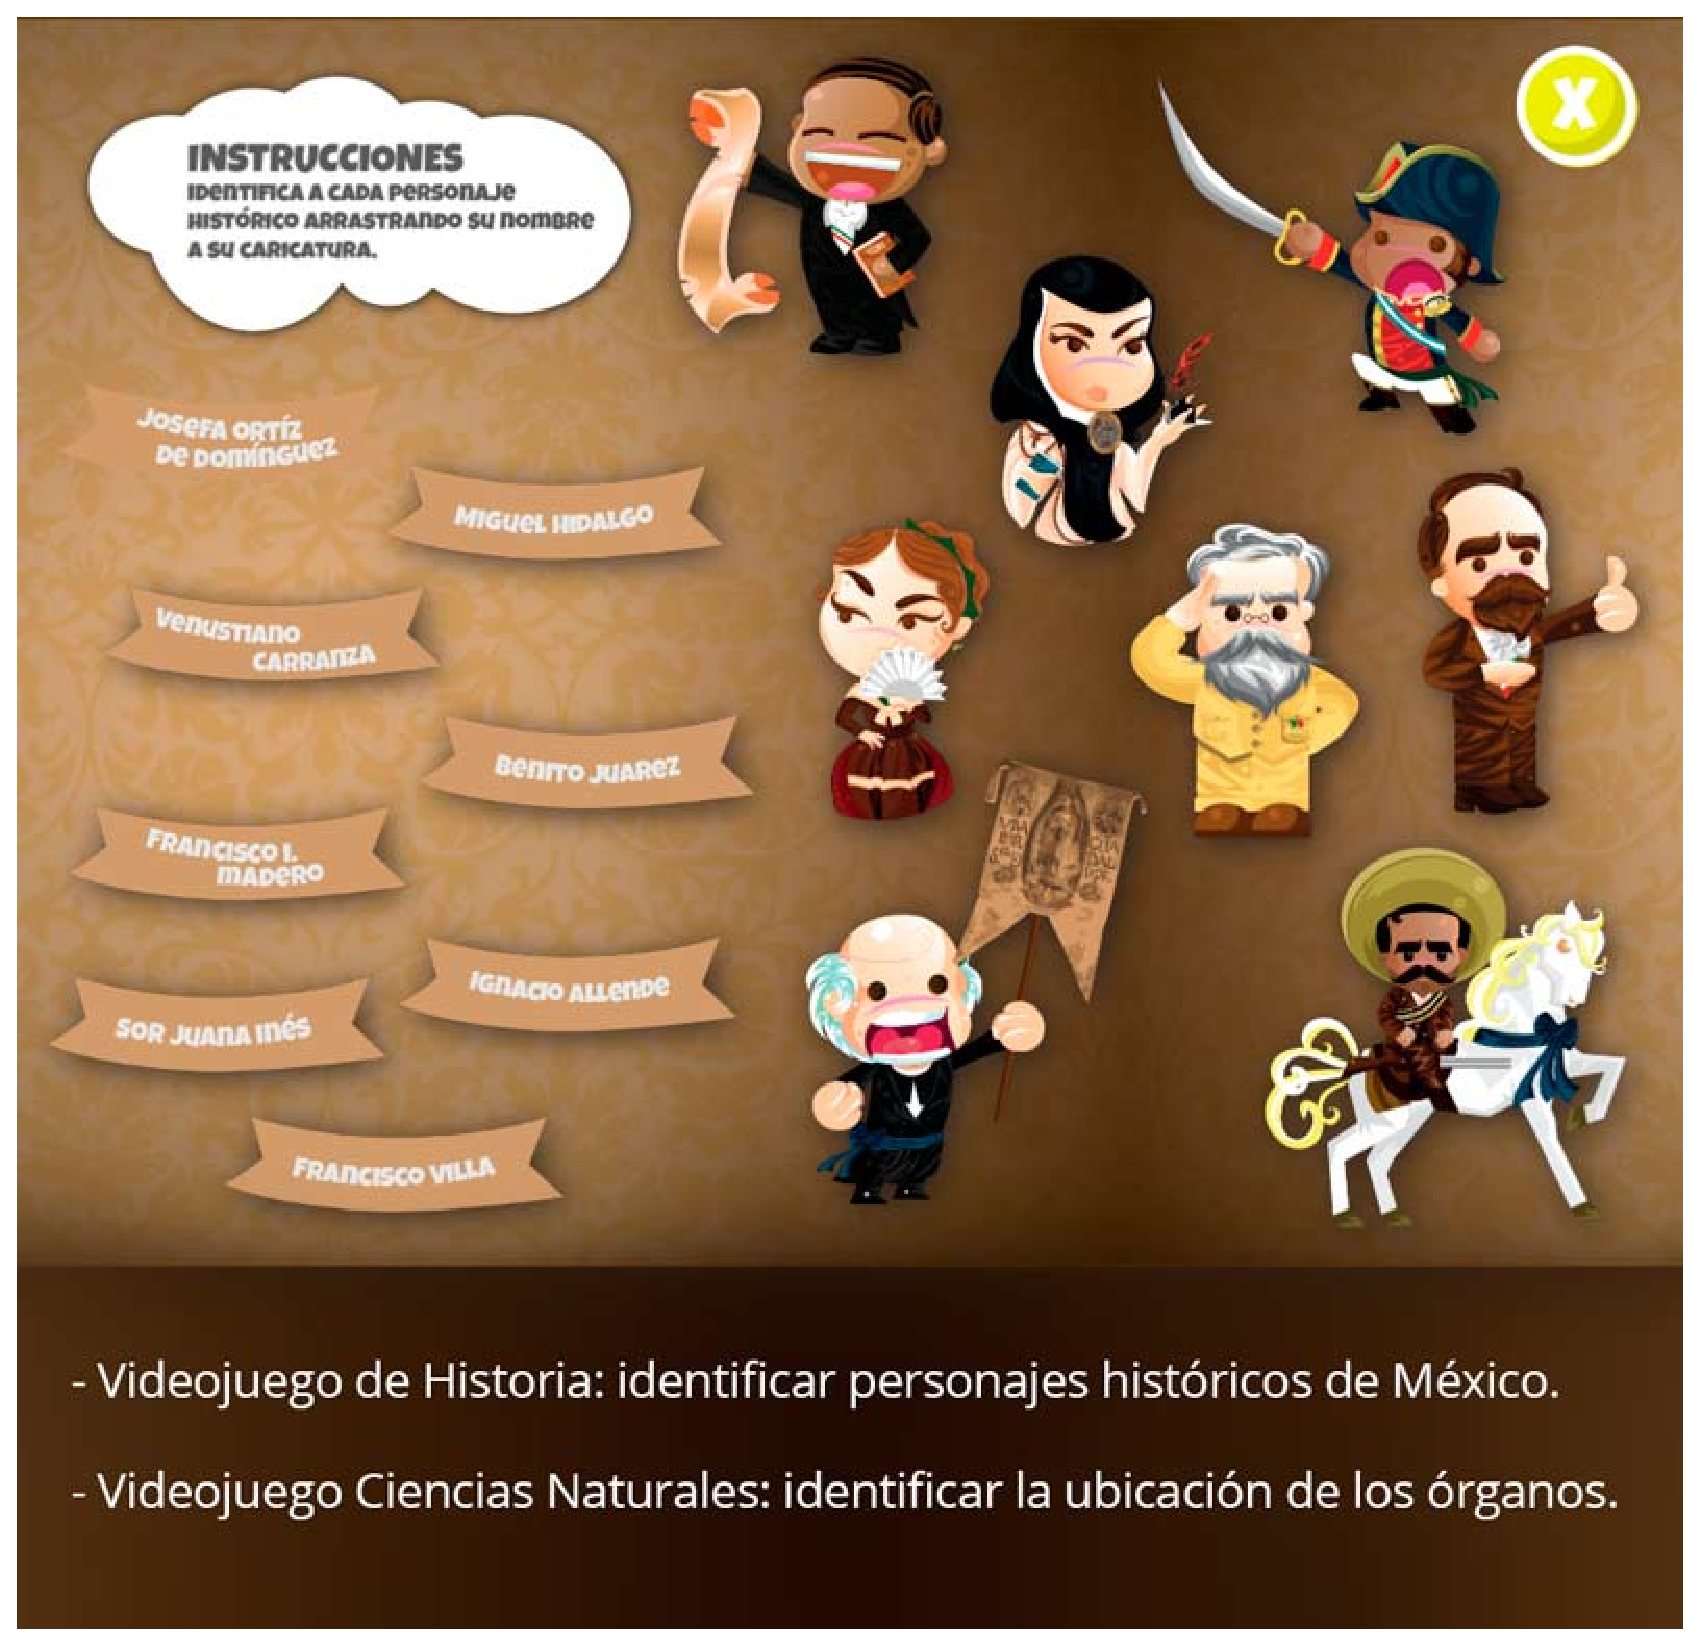
\includegraphics[width=0.5\textwidth]{03MarcoTeorico/imageR/learny}
\end{figure}

Como consecuencia el videojuego aumenta la motivación en el aprendizaje, ayuda al alumno a adquirir conocimientos de una manera atractiva y contribuye al desarrollo de competencias. Pero en contra parte, un videojuego educativo nunca podrá sustituir por completo la enseñanza tradicional como un salón de clases, un videojuego educativo sólo sirve como complemento y herramienta para el proceso de enseñanza-aprendizaje.
\\[1pt]

	
				
		
		
		
	\chapter{Estado del arte}

% Please add the following required packages to your document preamble:
% \usepackage{multirow}
A continuación presentamos en la tabla \ref{tab:tablaArte} nuestro producto propuesto en comparativa con algunos similares. Las características que mostramos son fecha de lanzamiento, la clasificación por género, edad del público al que va dirigido, la plataforma en la que se puede jugar, un apartado denominado tema que engloba el contexto del juego, el costo del producto y la compañía por la que ha sido realizado. Esto se muestra a fin de mostrar un panorama general de las diferencias y características que se tienen en el proyecto.
\begin{table}[htbp]
	\centering
	\caption{Tabla comparativa de juegos con características similares al producto propuesto. Notas: En desarrollo(ED), no determinado(-).}
	\label{tab:tablaArte}
	
	\resizebox*{\linewidth}{!}{
		\begin{tabular}{|l|l|l|l|l|l|l|l|l|l|l|l|l|l|l|l|l|l|l|l|l|l|l|}
			\hline
			\multicolumn{1}{|c|}{\multirow{2}{*}{Juego}} & \multirow{2}{*}{Fecha} & \multicolumn{8}{c|}{Género}                                                    & Edad  & \multicolumn{5}{c|}{Plataforma}                    & \multicolumn{3}{c|}{Tema}     & \multicolumn{1}{c|}{\multirow{2}{*}{Costo}} & \multicolumn{3}{c|}{Compañía}        \\ \cline{3-19} \cline{21-23} 
			\multicolumn{1}{|c|}{}                       &                        
			& \begin{sideways}Plataforma\end{sideways}
			& \begin{sideways}Metrodvania\end{sideways}
			& \begin{sideways}Puzzle\end{sideways} 
			& \begin{sideways} Lógica \end{sideways} 
			& \begin{sideways}Acción \end{sideways}
			& \begin{sideways}Aventura \end{sideways}
			& \begin{sideways}RPG \end{sideways}
			& \begin{sideways}Shooter \end{sideways} &  
			& \begin{sideways}PC \end{sideways}
			& \begin{sideways}Sony \end{sideways}
			& \begin{sideways}Microsoft \end{sideways}
			& \begin{sideways}Nintendo \end{sideways}
			& \begin{sideways}Móvil \end{sideways}
			& \begin{sideways}Ficción \end{sideways}
			& \begin{sideways}Fantasia \end{sideways}
			& \begin{sideways}Historia \end{sideways} & \multicolumn{1}{c|}{}                       
			& \begin{sideways}Estudio I. \end{sideways}
			& \begin{sideways}Independiente \end{sideways}
			& \begin{sideways}Ubisoft \end{sideways}
			\\ \hline
			
			Guacamelee! 2                                & ED                     & X          & X           &        &        & X      &          &     &         & 10+  &    & X    &           &          &       &         & X        &          & -                                           & X          &               &         \\ \hline
			Never Alone                                  & 2014                   & X          &             & X      &        &        &          &     &         & 10+  & X  & X    & X         & X        & X     &         & X        & X        & \$150                                       & X          &               &         \\ \hline
			Valiant Hearts                               & 2004                   &            &             &        & X      &        &          &     &         & 13+  & X  & X    & X         &          & X     & X       &          & X        & \$285                                       &            &               & X       \\ \hline
			Olimpya Rising                               & 2015                   & X          &             &        &        & X      &          &     &         & 10+  & X  &      &           & X        &       &         & X        & X        & \$95                                        & X          &               &         \\ \hline
			Jotun                      & 2016                   &            &             &        &        & X      & X        &     &         & 13+  & X  & X    & X         & X        &       &         & X        & X        & \$150                                       & X          &               &         \\ \hline
			Mulaka                                       & ED                     &            &             &        &        & X      & X        &     &         & -    & X  & X    & X         & X        &       &         & X        & X        & -                                           & X          &               &         \\ \hline
			MilitAnt                                     & 2016                   & X          &             &        &        & X      &          &     & X       & 10+  & X  & X    &           &          &       &         & X        &          & \$150                                       & X          &               &         \\ \hline
			Flat Kingdom                                 & 2016                   & X          &             &        &        & X      & X        &     &         & 10+  & X  &      &           &          &       &         & X        &          & \$100                                       & X          &               &         \\ \hline
			Viva Sancho Villa                            & 2015                   & X          &             &        &        & X      &          &     &         & 10+  &    &      &           &          & X     & X       &          &          & CI                                          & X          &               &         \\ \hline
			Heart Forth: Alicia                          & ED                     &            & X           &        &        &        &          & X   &         & -    & X  & X    &           & X        &       &         & X        &          & -                                           &            & X             &         \\ \hline
			Yolotl                                       & ED                     & X          &             &        &        & X      &          &     &         & 13+                   &    &      &           &          & X     &         & X        & X        & -                                           &            & X             &         \\ \hline
			
		\end{tabular}
	}
\end{table}
	\chapter{Alcance del proyecto}
En esta sección se definen el proyecto desde un punto de vista técnico; empezando 
por los objetivos del proyecto, su alcance, la metodología de trabajo, 
el cronograma de actividades, las especificación de la plataforma de desarrollo, 
el software requerido y los productos esperados. 
\section{Objetivos del proyecto} \label{Sec_ObjetivosPro}
En esta sección se habla de los objetivos, tanto generales cómo específicos, que persigue el presente trabajo terminal.
	\subsection{Objetivos generales}\label{Sec_ObjetivosGen}		
		\begin{itemize}
			\item Fomentar la cultura Mexica entre jóvenes mayores de 13 años a través de un videojuego.
		\end{itemize}
		
	\subsection{Objetivos especificos} \label{Sec_ObjetivosEsp}
		\begin{itemize}
			\item Realizar una investigación sobre la cultura Mexica.
			\item Diseñar un videojuego con bases históricas y mitológicas.
			\item Diseñar e implementar una narrativa que permita la difusión de la cultura Mexica. 
			\item Comprender el funcionamiento del motor del juego elegido.
			\item Entender el funcionamiento de un juego de plataforma básico.
		\end{itemize}
		
\section{Alcance del proyecto} \label{Sec_Alcance}
	El presente trabajo terminal tendrá:
		\begin{itemize}
			\item Funcionalidad de un solo usuario.
			\item Contener diez niveles, uno introductorio y nueve situados en el inframundo Mexica.
			\item Contar con sprites originales.
			\item Contar con un sistema de guardado, para salvar el progreso del jugador.
			\item Contener cinemáticas que cuentan una historia original.
			\item Funcionar en dispositivos android con los requerimientos expuestos en la sección \ref{Sec_Plataforma}.
			\item Contener un nivel que permite rejugar los niveles ya completados. 
		\end{itemize}
	El presente trabajo terminal no realizará:
	\begin{itemize}
		\item Enseñar historia.
		\item Realizar microtransacciones.
		\item Soportar múltiples jugadores.
		\item Contar con música original, creada especialmente para el juego.
	\end{itemize}
\section{Metodologia de trabajo}\label{Sec_Metodologia}
La metodología de trabajo elegida es Huddle. Como se mencionó en el apartado
 \ref{MetodoVideojuego}, Huddle es una metodología orientada a videojuegos y una
  de sus principales bondades que que ofrece la naturaleza iterativa de Scrum 
  con el agregado de cubrir la linea de producción de un videojuego 
  (ver apartado \ref{Pipelinevideojuego}).
\\
\par
El principal motivo por el que se eligió huddle, fue que es una metodología 
orientada a videojuegos; por lo que su documentación y sistema de trabajo cubre 
las necesidades de un proyecto de esta naturaleza y no es necesario hacer 
adaptaciones drásticas de la metodología tal como se tendrían que hacer si se 
hubiera elegido alguna de las metodologías orientadas a desarrollo de software 
como hubiera sido Scrum o programación extrema. 
\\
\par
Para consultar el cronograma de actividades del Trabajo Terminal, consultar el anexo \ref{}.

\section{Especificaciones de plataforma}\label{Sec_Plataforma}
En esta sección se enlistaran todos aquellos dispositivos de hardware y licencias
 de software que se necesitan para el desarrollo del vidoejuego.
 
 \subsection{Hardaware requerido}\label{Sec_PlataformaHw}
 En esta sección se mencionan los dispositivos de hardware empleados en el 
 desarrollo del sistema y los dispositivos de prueba del juegos. Estos 
 dispositivos son con los que se contaban a la hora de iniciar el Trabajo Terminal
 y no son sustituibles por motivos de presupuesto.
 	%================================================
 	\subsubsection{Computadoras para desarrollo}
 		\begin{itemize}
 			\item Computadora DELL Inspiron 15.
 				\begin{itemize}
 					\item Procesador Intel Core i3-4005U. 
 					\item CPU de 1.70 GHz de 64 bits. 
 					\item Memoria ram de 8GB.
 				\end{itemize}
			\item Lenovo G40. 
				\begin{itemize}
					\item Intel Core i3 4005U CPU 1.7 Khz de 64 bits. 
					\item Memoria ram de 8GB. 
					\item Tarjeta gráfica AMD Radeon R5 235 de 1GB
				\end{itemize}
 		\end{itemize}
 		
 	%===================================
 	\subsubsection{Dispositivos moviles de prueba}
 		\begin{itemize}   		
			\item Dispositivo de prueba 1:
		   		\begin{itemize}
		   			\item Versión 5.2
		   			\item Modelo Huawei TAG-L13
		   			\item CPU MediaTek MT6753 1,50 GHz
		   			\item IPS TFT 16M colors 720 x 1280 px (5,00) 294 ppi
		   			\item RAM 2GB	   			
		   		\end{itemize}
   		
   			\item Dispositivo de prueba 2:
		   		\begin{itemize}
		   			\item Versión 7.0
		   			\item Modelo ASUS X008DC
		   			\item CPU MediaTek Quad Core Processor
		   			\item GPU Mali T720
		   			\item RAM 3GB LPDDR3
		   			\item PANEL 5.2-inch
		   			HD(1280 x 720) IPS display 
		   			75 por ciento screen-to-body ratio
		   			400nits brightness 
		   		\end{itemize}   		  		
   		\end{itemize}


\subsection{Software requerido}
En este apartado se describen los softwares que se emplearán para el desarrollo 
del videojuego; cabe mencionar que todos los softwares mencionados en este apartado 
son empleados en el desarrollo haciendo uso de licencias de carácter individual, 
por lo que si se desea comercializar el videojuego, primeramente se debe de realizar  
un acuerdo comercial con las empresas proveedoras de las licencias. 
 
	\subsubsection{Motor de juego}
Como motor de juego se optó por Unity 3D en su versión 5.6.2.f1 como 
motor de juego en su licencia libre ya que no se cuenta con los fondos necesarios 
para contratar las versiones de pago. Los motivos por los que se eligió Unity 3D,
 son los que se presentan a continuación:
        \begin{itemize}
			\item Curva de aprendizaje rápida.
			\item Comunidad de desarrolladores activa.
			\item Permite gestionar trabajos 2D y 3D, esto permitirá escalar el juego 
                a 3D a futuro si alguien deseará retomar el proyecto.
			\item Codificación basada en el paradigma de programación orientada a
			objetos.
			\item Requerimientos técnicos de instalación dependientes del proyecto por
			lo que no exige una computadora de gran costo.
			\item Capacidad de desarrollo en múltiples plataformas, lo que permite la
                 escalabilidad futura del proyecto hacia nuevas plataformas en caso de
                 que alguien desee retomarlo.
        \end{itemize} 
A fin de garantizar la generación de los archivos apk de juego fue necesaria la instalación de Android Studio versión 2.3.3 y java en su versión  8u111.
	%================================
	\subsubsection{Creación de sprites}
Para la creación de sprites se eligieron dos softwares Corel Draw X5 y Adobe Photoshop. El primero se eligió para la vectorización de los sprites, ya que es de fácil uso, no requiere tantos recursos como Adobe Ilustrator y permite importar archivos a Adobe Photoshop para su posterior coloreado.
\\
\par
Tal como se mencionó en el párrafo anterior, el objetivo de Photoshop dentro de
 este trabajo terminal es colorear los sprites. El motivo para emplear photoshop
 es que permite la edición de imágenes y su optimizado para hacer sprites que 
 requieran menores tiempos de renderizado y menor espacio de almacenamiento sin
 sacrificar significativamente la calidad de la imagen.
	%================================	
	\subsubsection{Interfaz gráfica de usuario}
Para los iconos de los botones que controlan al usuario, se descargó una colección de botones del sitio web pixelsticky, este sitio web permite la descarga y utilización de diferentes iconos bajo la licencia de CC0 o de dominio público.

\section{Productos esperados}\label{Sec_Producto}
Los productos esperados se dividirán en dos, siendo los primeros los que se entregarán en al termino de Trabajo Terminal 1 y los segundos los que se entregarán al finalizar Trabajo Terminal 2.

\begin{itemize}
	\item Productos esperados al finalizar TT1:
		\begin{itemize}
			\item Documento de diseño.
			\item Guión literario del juego.
			\item Storyboard del juego.
			\item Documentación de la propuesta de diseño del juego.
			\item Maquetado de los niveles 1, 2, 3, 4.
			\item Niveles 1 y 2 terminado.
			\item Reporte técnico.
		\end{itemize}
	\item Productos esperados al finalizar TT2:
		\begin{itemize}
			\item Documentación del juego actualizada.
			\item Maquetado de los niveles 5, 6, 7, 8, 9 y 10.
			\item Nivel 3, 4, 5, 6, 7, 8, 9 y 10 terminados.
			\item Reporte técnico.
		\end{itemize}
\end{itemize}
	\chapter{Trabajo realizado}
	%%\input{05TrabajoRealizado/01DocDiseno}
	\section{Investigación histórica}

Antes de proceder a diseñar el juego, fue necesario realizar una investigación
sobre la cultura mexica y sobre la Malinche. En esta etapa, el principal reto 
que se tuvo que afrontar fue la cantidad de la información que existe sobre 
los mexicas; a pesar de que esta cultura es de las más estudiadas del México
prehispánico, si se le compara con culturas del sur y del norte del país, existe 
una discrepancia en cuanto a su historia y cultura entre los historiadores y 
estudiosos del tema, por lo que a la hora de tomar decisiones sobre la información 
a utilizar se tuvo que optar por alguna de las tantas versiones existentes sobre 
una misma historia.
	\\
	\par
	La investigación que se realizó se puede dividir en tres partes, con base al 
	objeto de estudio de la investigación:
	\begin{itemize}
		\item \textbf{Sociedad Mexica:} historia, tradiciones y clases sociales.
		\item \textbf{Mitología Mexica:} Mitos, leyendas, dioses.
		\item \textbf{Historia de la Malinche:} vida antes de la llegada de los 
		españoles.
	\end{itemize}
	
	En los siguientes apartados se hablará a mayor profundidad sobre la información 
	encontrada en cada parte de la investigación y sobre que información se decidió
	agregar como contenido al juego.
	\\
	\par
	Para mayor comprensión sobre algunos de los puntos expuestos en esta 
	sección, se le recomienda al lector consultar los apartados de personajes y 
	guión en el documento de diseño.
	
	\subsection{Sociedad Mexica}
	La información que se decidió poner en el juego referente a la sociedad Mexica 
	fue referente a aquella que ayude al jugador a darse una idea sobre el contexto 
	que se vivía en esa época y las interacciones sociales que existían entre 
	individuos y culturas. 
	\\
	\par		
	Primeramente se encontró que, antes de la llegada de los españoles, México como 
	nación no existía, sino que en el territorio en donde convivían diversos pueblos 
	con rasgos culturales diversos y que en su gran mayoría estaban enemistados
	\cite{RefMexicasMito}. Esto llevó a la decisión de mostrar a los Mexicas como el 
	imperio conquistador que fue, mostrando a su vez el descontento que existía en los 
	pueblos conquistados por el imperio.
	\\
	\par
	 El segundo dato encontrado que se consideró de gran importancia, fue la 
	 organización de las clases sociales de los Mexicas y la gran importancia que 
	 tenia esa división social en la vida cotidiana; determinando no solo los 
	 derechos de los habitantes de aquella época, sino a su vez determinaba vestimenta 
	 y comportamiento \cite{RefCivilAztea}. Esta información fue considerada relevante 
	 ya que influenciaría en el diseño de personajes para denotar su rango y 
	 personalidad.
	 \\
	 \par
	 Otro dato importante que influenció el diseño del juego fue la importancia que 
	 tenía el comercio en aquella época, al ser un medio de intercambio de mercancías
	 e información \cite{RefMexicasMito}. Esta información resultaría determinante a la 
	 hora de elegir la locación del nivel introductorio y su posterior diseño.
	 
	 \subsection{Mitología Mexica} 
	 La mitología Mexica es basta y muy extensa. Los Mexicas contaban con sus propios 
	 mitos y dioses y a estos se les fueron integrando a sus creencias los mitos y
	  deidades de los pueblos que conquistaban. Dentro de sus principales deidades 
	  se encontraban \textit{Tezcatlipoca}, \textit{Quetzalcóatl} y 
	  \textit{Huitzilopochtli} \cite{RefMexicasSol}.
	 \\
	 \par
	 Para el diseño del argumento del videojuego se tomaron diferentes mitos y creencias
	 de los Mexicas, a continuación se mencionan, describiendo brevemente en que
	 consisten y como impactaron el videojuego:
	 \begin{itemize}
		\item \textbf{El mito de los cinco soles:} En este mito se narran la diferentes 
		creaciones y destrucciones del mundo a manos de los dioses\cite{RefMexicasMito}. 
		Este mito permitió la plantear una historia anterior al juego y de darle una 
		identidad al mundo de los dioses al implementar una jerarquía de deidades 
		similar a la de la sociedad Mexica.
		%===============================================
		\item \textbf{El mito de la creación del hombre del maíz:} Mito que habla como 
		\textit{Quetzalcóatl} y el Dios \textit{Xólotl} descienden al \textit{Mictlán}
		 y cumplen una serie de retos para lograr hacerse de los huesos de la anterior 
		 humanidad y así crear a la actual\cite{RefMexicasMito}. Este mito es de gran 
		 importancia ya que la idea conceptual del juego nació de este.
		 %===============================================
		\item \textbf{El \textit{Mictlán}:} Este lugar era el equivalente al inframundo
		dentro del pensamiento cristiano. El \textit{Mictlán} estaba constituido por 
		nueve niveles, cada uno vigilado por una deidad. Los difuntos iban a este lugar 
		para purificarse y volver a ser \textit{tonalli}(alma), lo que les permitía 
		volver a ser uno con el mundo. Le viaje al \textit{Mictlán} duraba cuatro años, 
		y durante su duración el difunto debía de afrontar una diferentes retos en 
		cada uno de los niveles del \textit{Mictlán}\cite{RefMexicasSol}. Este lugar 
		mitológico influenció fuertemente el diseño del videojuego, al determinar 
		mecánicas de juego, enemigos y la cantidad de niveles que el juego tiene. En 
		cuanto a los enemigos, se decidió incluir algunos Dioses que no eran propios 
		del \textit{Mictlán} pero que por sus habilidades o simbologia se les podía 
		relacionar con este; el objetivo de proponer deidades fue para ofrecer una 
		variedad de dioses y que el jugador pudiera conocer dioses no tan famosos de la 
		mitología Mexica.    
	 \end{itemize}	 
	 
	 \subsection{Historia de la Malinche}   
	 La \textit{Malinche} es una de las figuras más controversiales de la historia 
	 mexicana. La investigación sobre su historia antes de la llegada de los españoles
	 resultó tan interesante que repercutió en el trabajo, haciendo que el personaje 
	 histórico se transformara el una de las figuras centrales de la narrativa y en la 
	 protagonista del juego. La figura de Malinche será manejada a lo largo del 
	 argumento del juego sin decirle al jugador quien es en realidad la protagonista 
	 es del juego, planeando revelar su identidad como un giro argumental de la trama.




	\section{Diseño del juego}\label{docDisenio}
Como parte de la etapa preproducción de la metodología Huddle, se redactó el documento de diseño. En este documento se definieron todos aquellos elementos de jugabilidad, diégesis y narrativa que le dan identidad al juego, de igual forma se definieron aspectos técnicos y de funcionalidad que permiten proponer un diseño del juego basado en el paradigma de programación orientada a objetos.

%===========================================
\subsection{Idea concepto.}
Si bien la metodología propone un orden en el que se debe de llenar el documento de diseño, es importante aclarar que este orden puede o no seguirse. Lo anterior se debe a la naturaleza creativa y multidisciplinaria del videojuego; lo ocasiona que la idea principal del juego (el concepto) pueda venir bien de la idea de una mecánica de juego o de un argumento. En el caso del juego Yolotl, el juego nació primero como un argumento y después el argumento dió origen a la mecánica por lo que los primero rubros en llenarse fueron aquellos relacionados con la diégesis y el argumento del juego. 
\\
\par
Originalmente, Yolotl narraría la travesía de un guerrero en el Mictlán con el fin de traer de vuelta a la vida a su hermano. Con esta primera idea se propusieron cuatro niveles y una mecánica de juego más orientada a la resolución de puzles y al combate con diferentes armas. Desafortunadamente, esta primera idea jamás termino de aterrizarse y fue abandonada parcialmente. Apoyándose del fomento a la cultura se procedió a crear un nuevo argumento, esta vez con bases históricas más sólidas a fin de permitirle al jugador no solo interactuar con la cosmovisión de los Mexicas sino a su vez con el entorno social de los mismos. Conceptos como el viaje al Mictlán y el pacto con un Dios para revivir a un ser querido fueron algunas de las ideas que se mantuvieron con la segunda idea argumental del juego. 


%===========================================
\subsection{Concepto del juego.}
Una vez definido el concepto general del argumento se procedió a definir 
las especificaciones técnicas y de jugabilidad del juego. En este punto se 
inició a escribir el documento de diseño en el orden que propone la plantilla 
de la metodología. 
\\
\par
En el primer apartado del documento de diseño se definió el concepto del juego. 
La primera decisión que se tomó en este apartado fue el género de videojuego que 
se desarrollaría, siendo elegida una combinación de dos géneros: plataforma y 
aventura. El principal motivo por el que se eligieron dichos géneros fue su 
complejidad, ya que siendo un equipo de dos personas y considerando el tiempo 
disponible de desarrollo, elegir géneros que requerían una mayor complejidad 
como RPG o Shooter minimizarían significativamente la factibilidad del juego.  
\\
\par
Posteriormente se redactó una sinopsis del contenido del juego de jugabilidad e 
historia del juego; más tarde en el mismo apartado la jugabilidad se describió 
de manera más detallada en la sección de mecánica de juego, en donde se 
definieron las acciones básicas del personaje principal y algunas de las reglas 
que rigen el comportamiento del juego a lo largo de todos los niveles. 
\\
\par
En este apartado también se definieron las tecnologías, tanto en hardware como 
en software, a utilizar para el desarrollo, eligiendo como plataforma dispositivos 
móviles con un mínimo de requerimientos técnicos que el teléfono Huawei TAG-L13 
con sistema Android 5.2, esto debido a que el mercado de los juegos para 
dispositivos móviles es el que cuenta con mayor demanda\cite{Ref_IndusMEx}; en 
cuanto a software se eligió a Unity como motor de desarrollo por la 
características ya mencionadas en (ver apartado \ref{Sec_PlataformaHw}). 
\\
\par
Finálmente se definieron aspectos legales y comerciales como el tipo de licencia 
de distribución a Atribución-NoComercial-CompartirIgual CC BY-NC-SA y el público 
objetivo del juego a jóvenes mayores de 13 años. Este último rubro no solo delimitó 
el contenido argumental del juego y sus mecánicas sino que también fungió como un 
factor determinante para decidir un comportamiento totalmente offline, esto 
debido a que se busca cumplir con los lineamientos establecidos por el Acta de 
Protección de la Privacidad de los Niños En Línea (C.O.P.P.A. por sus siglas en 
inglés), la cual es una Organización encargada de la protección de la información 
de los menores de trece años \cite{RefCOPPA}. 

%===========================================
\subsection{Mecánica de juego.}
El siguiente apartado que aportó información significativa al diseño del juego, 
fue el de la Mecánica del juego, pues en éste se definieron aspectos técnicos 
que garantizarían el funcionamiento de la mecánica de juego descrita en el 
primer apartado, tales como la cámara, los periféricos, los controles y el 
guardado y carga de datos. 
\\
\par
La cámara se definió como una cámara de perspectiva ortogonal lateral que seguiría 
el movimiento en ambos ejes coordenados (Ver figura \ref{fig:Camara}).

\begin{figure}
  \centering
  \subfigure[Seguimiento horizontal]{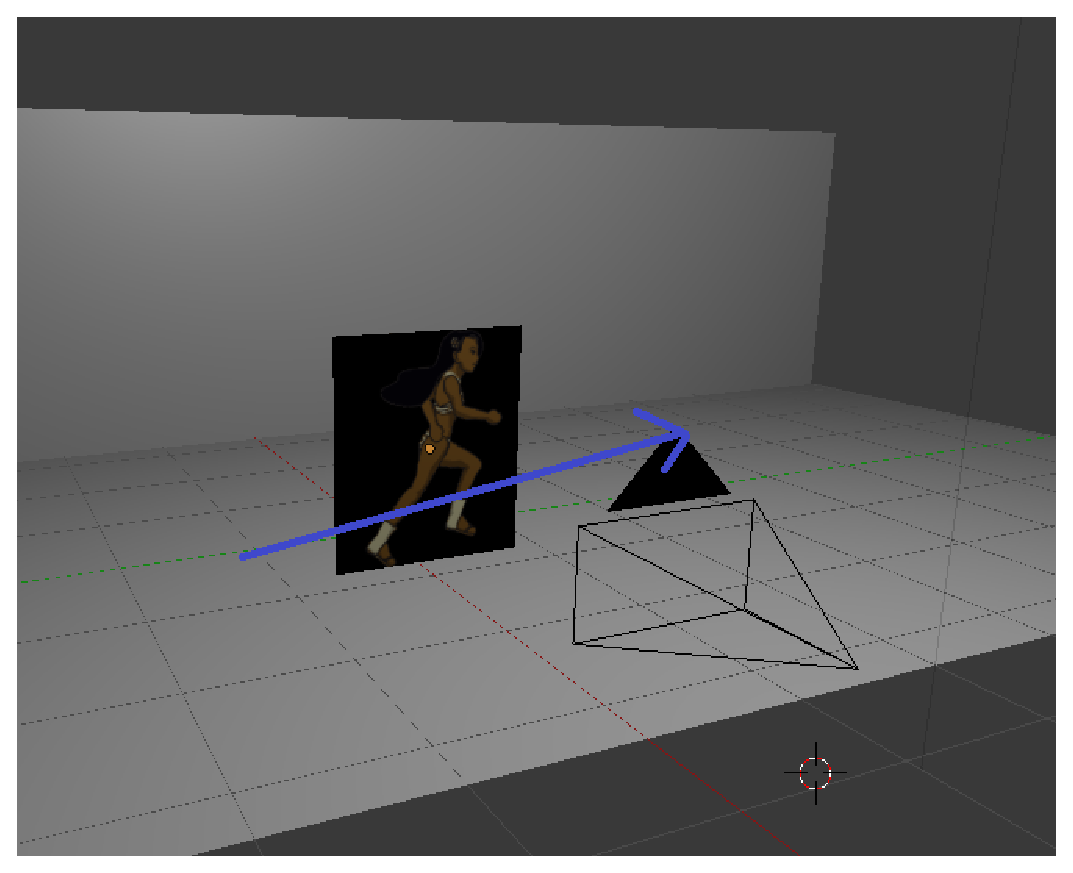
\includegraphics[width=0.7 \textwidth]{05TrabajoRealizado/01DocDiseno02/imagenes/camara01}}
   \subfigure[Seguimiento vertical.]{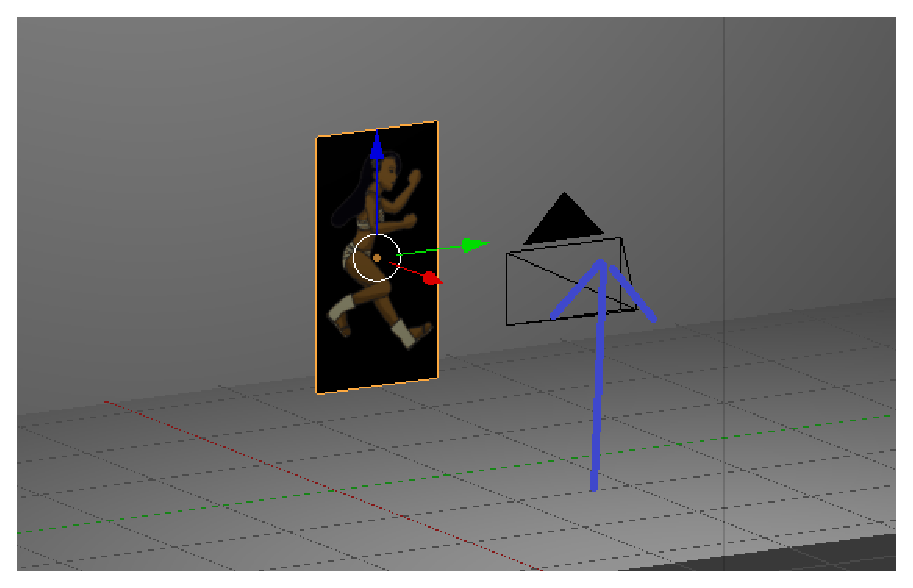
\includegraphics[width=0.7 \textwidth]{05TrabajoRealizado/01DocDiseno02/imagenes/camara02}}
  \caption{La cámara seguirá la posición del jugador en el eje x y y.}
  \label{fig:Camara}
\end{figure} 
 

\par
Por su parte, los controles del juego se establecieron como un conjunto de cuatro 
botones (Ver figura \ref{fig:GUI} ); cada uno con una acción específica a 
desempeñar: mover hacia la izquierda, mover hacia la derecha, disparar, hablar, 
saltar. Siendo periférico o el medio de interacción de los botones y el jugador 
la pantalla táctil del teléfono.  

\begin{figure}
				\centering
				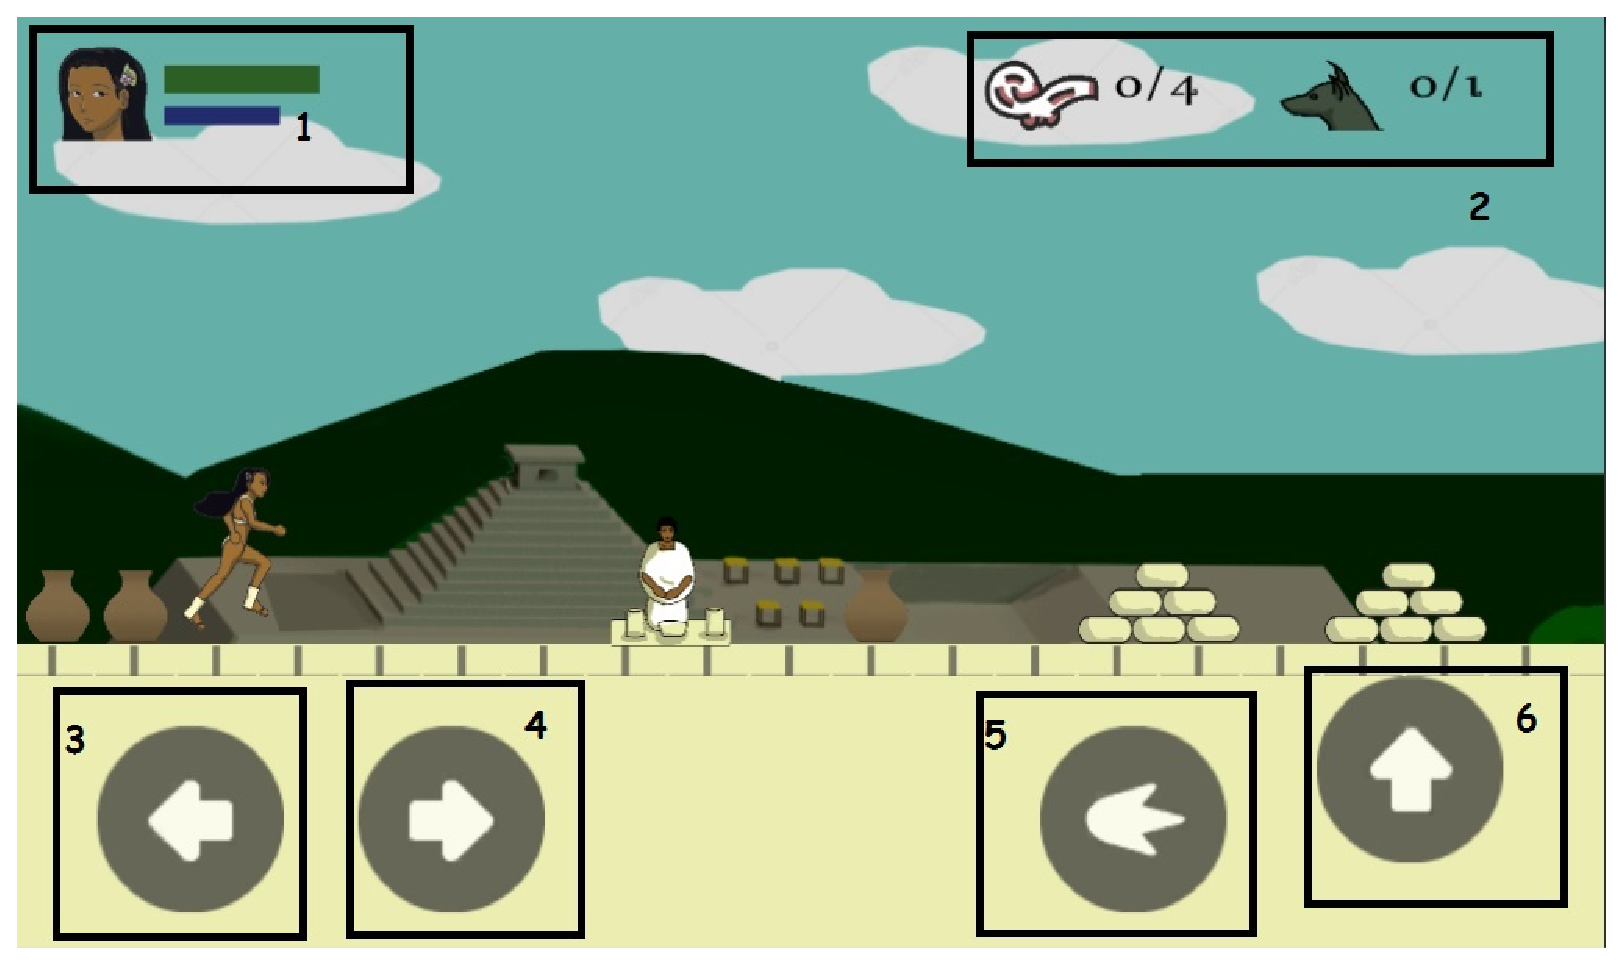
\includegraphics[height=0.3 \textheight]{05TrabajoRealizado/01DocDiseno02/imagenes/ControlCorrerDer}
				\caption{1 Información del personaje jugable, barra verde indicador 
				de la cantidad de vida, barra azul cantidad de tonalli. 2 Objetivos 
				del nivel o información útil. 3 Botón moverse izquierda. 4 Botón 
				moverse derecha. 5 Botón disparar tonalli. 6 Botón saltar.}
				\label{fig:GUI}
\end{figure}


\par
En cuanto al guardado y la carga, se propusieron dos tipos guardado y carga automática 
y guardado y carga de checkpoint; el primero guarda el progreso del jugador al 
completar el nivel y permite inicializar los niveles desbloqueados y el segundo 
se utiliza dentro de un nivel para guardar el progreso del jugador en el nivel 
en caso de que muera pueda iniciar desde el último checkpoint que tocó. 
Si el lector de este documento dese profundizar más en lo anteriormente dicho, 
se le recomienda consultar el Capítulo 5 del documento de diseño.
%===========================================
\subsection{Interfaces}\label{TraReaInterfaces}
Para la navegación dentro del juego, se diseñaron tres interfaces gráficas: 
La pantalla de inicio, Menú principal y el menú de selección de nivel. 
A continuación, se hará una breve descripción de la función principal de 
las interfaces:
\begin{itemize}
	\item\textbf{ Interfaz de inicio:} Presenta el logo del juego y la información 
	legal del mismo, sirve como pantalla de introducción al juego. Conecta con 
	la interfaz de menú principal (Ver figura \ref{fig:PInicio} ) .
	\item \textbf{Interfaz de menú principal:} Muestra la misma ilustración que la 
	pantalla de inicio, con la diferencia de que muestra dos botones en la parte 
	inferior izquierda de la pantalla. Con estos botones se puede empezar una nueva 
	partida o cargar una ya existente. Esta interfaz conecta a la cinemática de 
	inicio del juego si el jugador oprime el botón de empezar partida y confirma 
	que desea empezar una partida nueva o direcciona a la interfaz de menú de 
	selección de nivel, si el jugado oprime el botón de cargar partida y existe 
	un archivo con los datos del juego (Ver figura \ref{fig:PMenuP}).
	\item \textbf{Interfaz de Menú selección de nivel:} En esta interfaz el 
	jugador podrá elegir el nivel que desea jugar, siempre que lo haya desbloqueado 
	con anterioridad (Ver figura \ref{fig:SelNivel}).
\end{itemize}

\begin{figure}
  \centering
   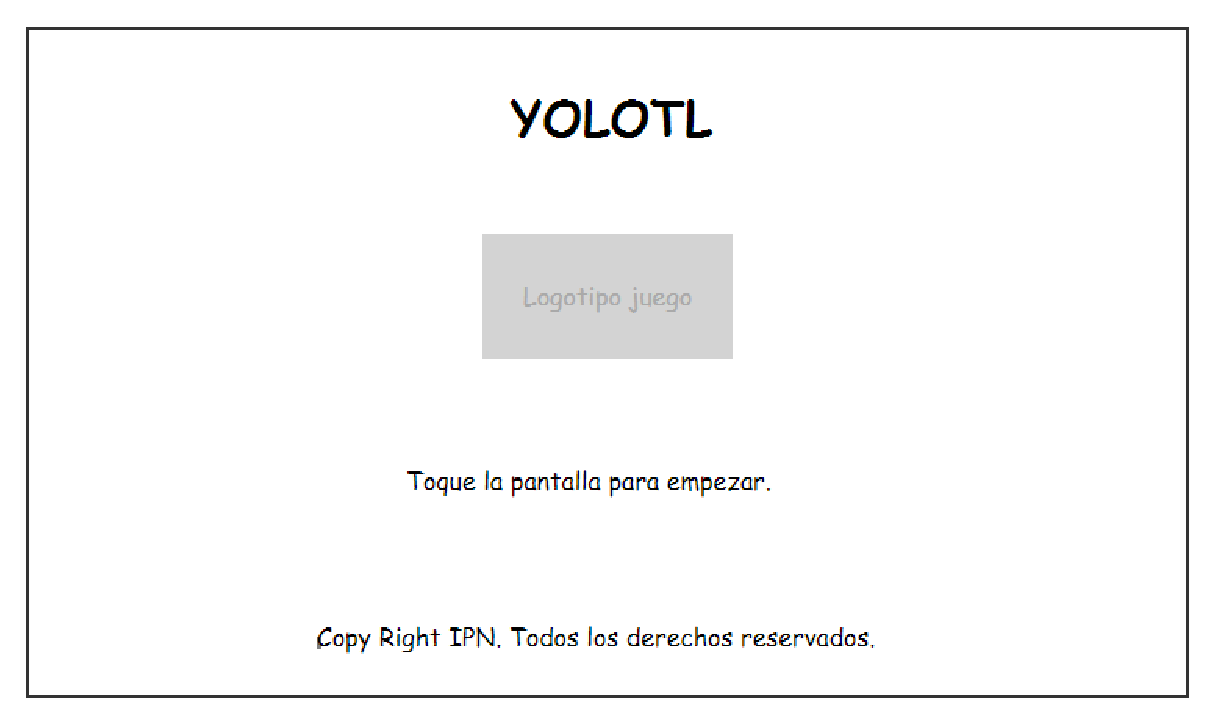
\includegraphics[width=0.6 \textwidth]{05TrabajoRealizado/01DocDiseno02/imagenes/interfaz00}
  \caption{Interfaz 1.0 Pantalla de inicio.}
  \label{fig:PInicio}
\end{figure} 


\begin{figure}
  \centering
   \subfigure[Menú principal] {\includegraphics[width=0.6 \textwidth]{05TrabajoRealizado/01DocDiseno02/imagenes/interfaz01}}
   
 	\subfigure[Cuadro de dialogo para confirmar iniciar nueva partida.] {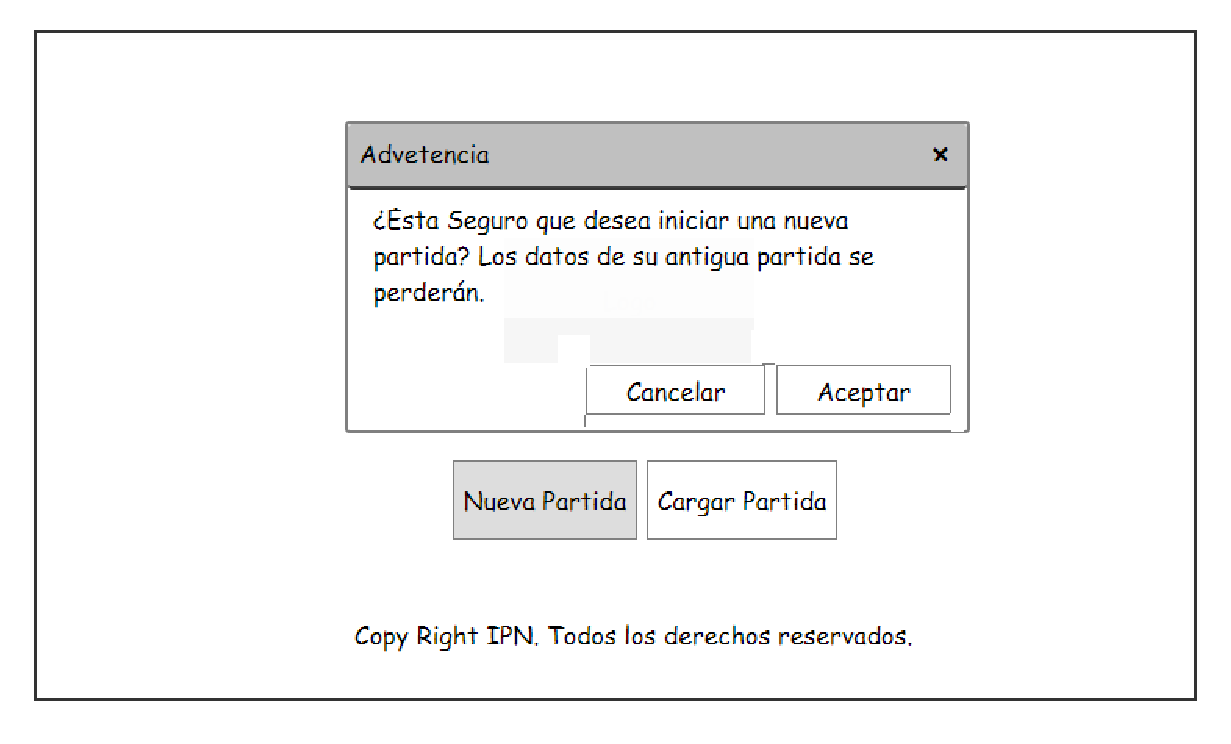
\includegraphics[width=0.6 \textwidth]{05TrabajoRealizado/01DocDiseno02/imagenes/interfaz01_02}}
 	
\subfigure[Cuadro de dialogo cuando no existen partidas que cargar.] {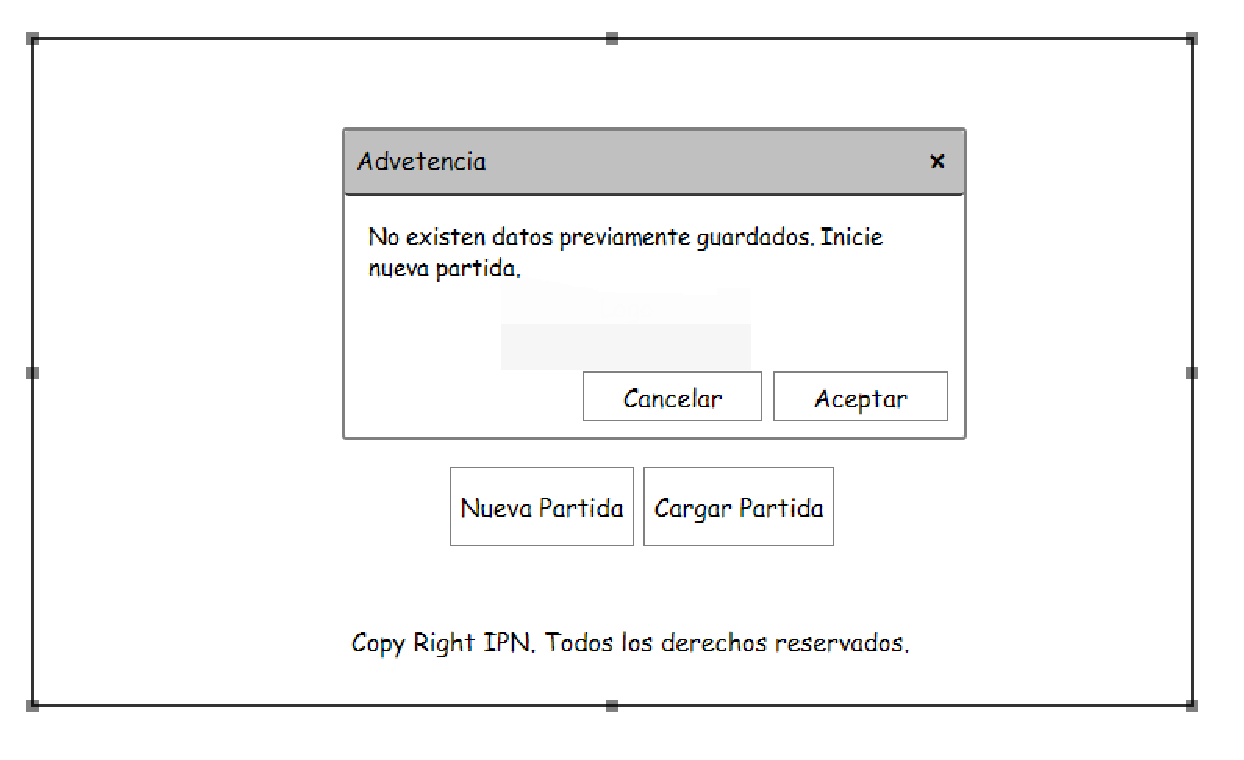
\includegraphics[width=0.6 \textwidth]{05TrabajoRealizado/01DocDiseno02/imagenes/interfaz01_03}}
  \caption{Interfaz 2.00 Menú principal.}
  \label{fig:PMenuP}
\end{figure} 


\begin{figure}
  \centering
   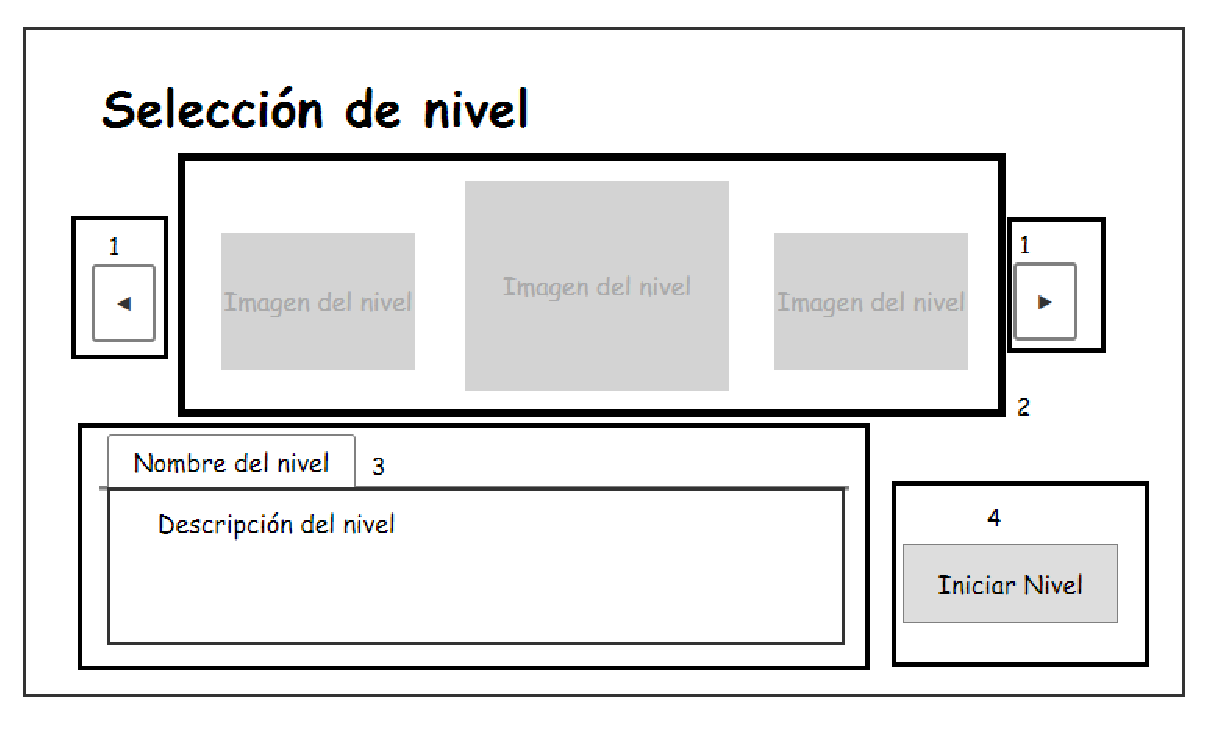
\includegraphics[width=0.6 \textwidth]{05TrabajoRealizado/01DocDiseno02/imagenes/interfaz02_01}
  \caption{Interfaz 2.00 Selección de nivel.1 botones que controlan el carrusel. 2 Carrusel. 3 Información del nivel seleccionado. 4 Botón Iniciar nivel.}
  \label{fig:SelNivel}
\end{figure}  
%===========================================
\subsection{Niveles.} \label{Niveles}
Yolotl es un juego compuesto por diez niveles: un nivel introductorio y los nueve 
niveles del inframundo.  Dado que la idea concepto del juego Yolotl lo situa en 
el Mictlán, la cantidad mínima esperados seria nueve; sin embargo, se tomó la 
decisión de incluir un nivel de introducción debido a los siguientes factores: 

\begin{itemize}
	\item Introducir al jugador a las mecánicas de juego básicas antes de lanzarlo 
	a un nivel más complicado.
	\item Situar el juego dentro de un contexto histórico real, permitiéndole al 
	jugador conocer sobre la sociedad Mexica de una manera en la que el jugador 
	pueda ser participe de este contexto histórico.
	\item Seguir una estructura narrativa básica en la que se presente la vida 
	cotidiana del héroe antes del llamado a la aventura \cite{RefHeroe}.
\end{itemize}

Usualmente, en el juego de Yolotl, un nivel está compuesto de dos secciones: una 
sección de obstáculos y plataformas en donde cumplirá un objetivo propio del nivel 
y otra donde el jugador se enfrentará al enemigo jefe del nivel. A excepción 
del primero y ultimo nivel el resto de los niveles siguen esa estructura. En el 
caso del primer nivel sigue la división de las dos secciones, con la diferencia 
de que no existe un enemigo jefe a vencer en la segunda sección del nivel; 
mientras que en el último nivel existe una única sección en donde el jugador 
se enfrentará a las diferentes transformaciones del jefe final.
\\
\par
La progresión entre niveles es lineal (Ver figura \ref{fig:ProgreNiveles}), 
por lo que no se puede acceder al nivel determinado sin antes haber completado 
a su predecesor; siendo el primer nivel, el que se encuentra disponible de manera 
estándar al empezar una nueva partida. Un nivel se da completado únicamente 
hasta que se ha derrotado al enemigo jefe del nivel; salvo por el primer nivel, 
el cual se considera terminado una vez que el jugador obtiene el arma de la 
protagonista. Cuando el jugador completa un nivel, además de desbloquear el 
siguiente nivel, el jugador podrá ver determinadas cinemáticas con las que podrá 
seguir la historia del juego y obtiene mejoras sobre alguno de los atributos del 
personaje.
\\
\par
En la tabla se encuentra información referente a cada nivel tal como los 
objetivos a cumplir, el enemigo a vencer, lo que se obtiene al completar el nivel.

%%============== PROGRECION DE NIVELES ==============
\begin{figure}
  \centering
   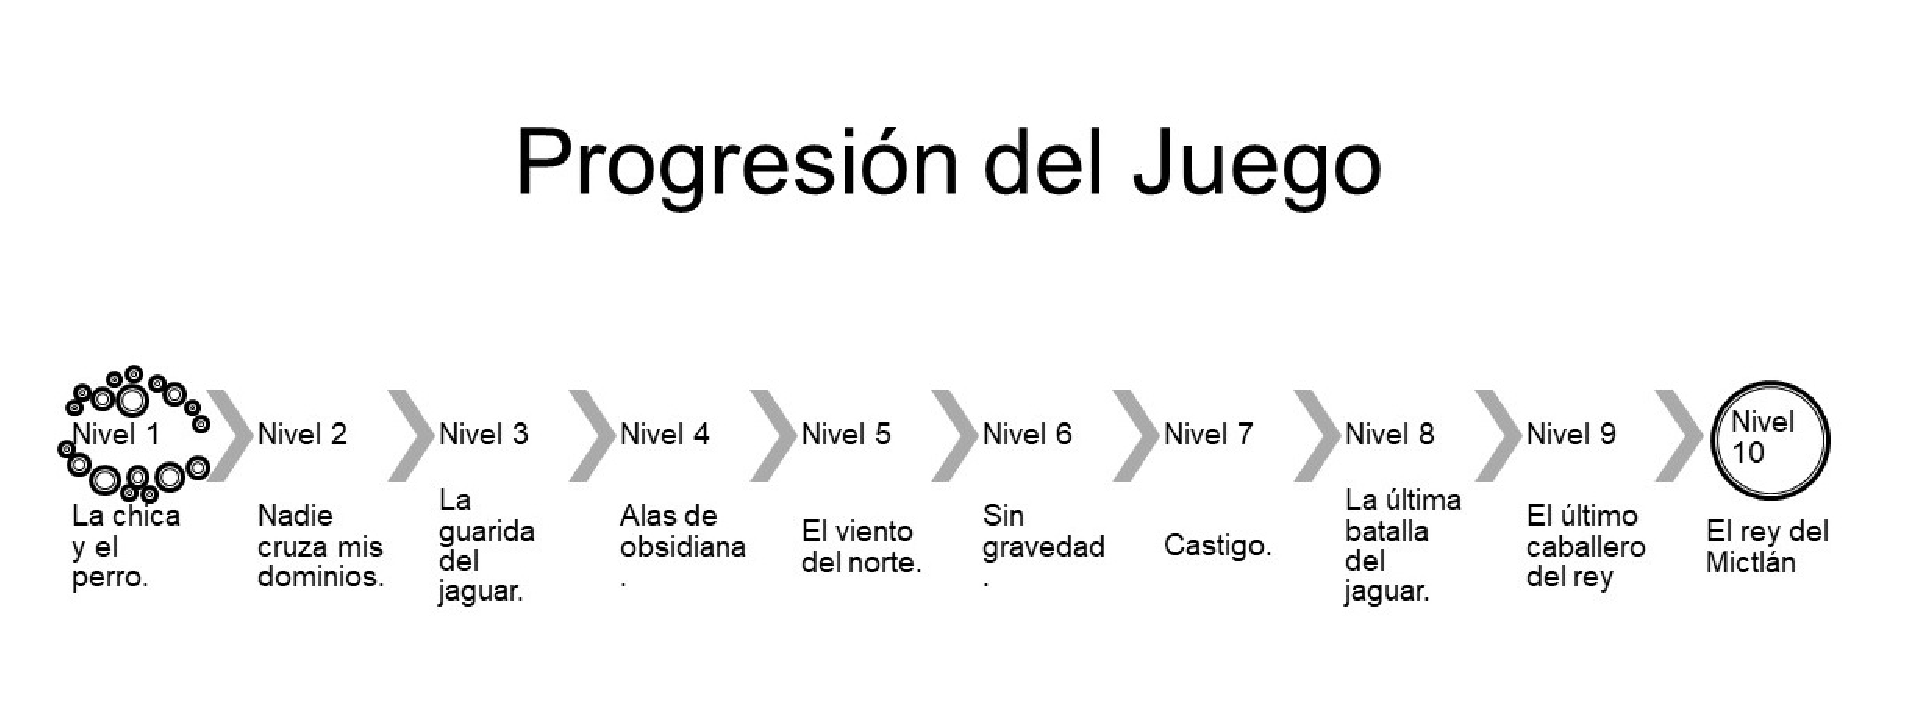
\includegraphics[width=0.8 \textwidth]{05TrabajoRealizado/01DocDiseno02/imagenes/ProgresJuego}
  \caption{Progresión del juego}
  \label{fig:ProgreNiveles}
\end{figure} 

%%============== TABLA DE NIVELES =============
%\begin{table}
	\begin{longtable}[c]{ | m{3.75cm} | m{3.75cm}| m{3.75cm} | m{3.75cm}|} 
		%\endhead		
		%\endfirsthead
		%\endlastfoot
		%\hline
		\rowcolor{cyan} Nivel.& Objetivo & Zona de plataformas	Enemigo jefe & Progreso obtenido. \\ 
		\hline
		%-------------------------------
		Nivel 1 “La chica y el perro”. & 
		Hablar con al menos cuatro ciudadanos.
			\par 
			Interactuar con Xólotl.
			\par 
			Obtener la caracola.&
		Sin enemigo jefe.&
		 Nivel 1.
			\par 
			Cinemática 3.
			\par 
			Cinemática 4.
			\par 
			Habilidad de disparo.		 
		 \\ 
		\hline
		%-------------------------------
		Nivel 2 “Nadie cruza mis dominios”. & 
		Atravesar el rio evitando tocar a los Xoloitzcuintles, por cada Xoloitzcuintles tocado incrementara el poder de Xochitónal. &
		Xochitónal. &
		Mejora en la cantidad de vida de Malinalli.
			\par 
			Cinemática 6.
			\par 
			Cinemática 7.
			\par 
			Cinemática 8.
			\par 
			Cinemática 9.
			\par 
			Cinemática 10.
			\par 
			Nivel 3.		 
		 \\ 
		\hline
		%-------------------------------
		Nivel 3 “La guarida del jaguar”. & 
		Llegar a la guarida de Tepeyóllotl. &
		Tepeyóllotl. &
		Mejora en la cantidad de Tonalli de Malinalli.
			\par 
			Cinemática 12.
			\par
			Cinemática 13.
			\par 
			Cinemática 14.
			\par
			Nivel 4.		 
		 \\ 
		\hline
		%-------------------------------
		Nivel 4 “Alas de obsidiana”. & 
			Encontrar el camino correcto hacia la guarida de Itzpapálotl.
			\par
			Encontrar las tres llaves que abren la puerta de la guarida de Itzpapálotl.&
		Itzpapálotl. &
			 Mejora en la cantidad de vida de Malinalli.
			 \par
			 Cinemática 16.
			 \par
			 Cinemática 17.
			 \par
			 Cinemática 18.
			 \par
			 Cinemática 19.
			 \par
			 Cinemática 20.
			 \par
			 Cinemática 21.
			 \par
			 Cinemática 22.
			 \par
			 Nivel 5.		 
		 \\ 
		\hline
		%-------------------------------
		Nivel 5 “El viento del norte”. & 
		Llegar a la guarida Mictlecayotl.&
		Mictlecayotl. &
		Mejora en la cantidad de Tonalli de Malinalli.
		\par
		Cinemática 24.
		\par
		Cinemática 25.
		\par
		Cinemática 26.
		\par
		Cinemática 27.
		\par
		Nivel 6.		 
		 \\ 
		\hline
		%-------------------------------
		Nivel 6 “Sin gravedad”. & 
		Llegar a la guarida Tlazoltéotl &
		Tlazoltéotl. &
		Mejora en la cantidad de vida de Malinalli.
		\par
		Cinemática 29.
		\par
		Cinemática 30.
		\par
		Cinemática 31.
		\par
		 Nivel 7.		 
		 \\ 
		\hline
		%-------------------------------
		Nivel 7 “Castigo”. & 
		Llegar a la guardia Itztlacoliuhqui. &
		Itztlacoliuhqui. &
		Mejora en la cantidad de Tonalli de Malinalli.
		\par
		Cinemática 33.
		\par
		Cinemática 34.
		\par
		Cinemática 35.
		\par
		Nivel 8.		 
		 \\ 
		\hline
		%-------------------------------
		Nivel 8 “La última batalla del jaguar”. & 
		Llegar a la guarida de Tepeyóllotl.&
		Tepeyóllotl. &
		Mejora en la cantidad de vida de Malinalli.
		\par		
		Cinemática 37.
		\par
		Cinemática 38.
		\par
		Cinemática 39.
		\par
		Nivel 9.		 
		 \\ 
		\hline
		%-------------------------------
		Nivel 9 “El último caballero del rey”. & 
		Superar la zona de Tula.
		\par
		Superar la zona de Oluta.&
		Nexoxcho. &
		Mejora en la cantidad de Tonalli de Malinalli.
		\par		
		Cinemática 44.
		\par
		Cinemática 45.
		\par
		Cinemática 46.
		\par
		Nivel 10. 
		 \\ 
		\hline
		%-------------------------------
		Nivel 10 “El rey del Mictlán”. & 
		Sin objetivos &
		Mictlantecutli. &
		Cinemática 47.
		\par		
		Juego terminado. 
		 \\ 
		\hline
	\end{longtable}

	%\caption{Información de los niveles.}
	%\label{Tab:Niveles}
%\end{table}
%===========================================
\subsection{Obstáculos}
De manera particular, para el proyecto Yolotl, se entiende por obstáculos a aquellos objetos dentro de un nivel que dificultan el avance continuo del jugado o que faciliten el fallo del jugador.
\\
\par
A diferencia de los personajes, la metodología huddle no maneja una plantilla para documentar estos objetos, por lo que se propuso una plantilla propia. Los campos de la plantilla son:
	\begin{itemize}
		\item Nombre del obstáculo.
		\item Descripción: Este campo describe tanto físicamente el objeto como su comportamiento e interacción con el jugador. 
		\item Esquema: Imagen de apoyo que facilita la comprensión de la descripción. 
	\end{itemize}
En total se definieron alrededor de 11 obstáculos, mismos que se podrán encontrar repartidos a lo largo de los niveles del juego. Algunos obstáculos serán exclusivos de un nivel mientras que otros se podrán encontrar en todos los niveles.
 \\
 \par
 A continuación se listarán los obstáculos del juego:
 	\begin{itemize}
 		\item Caja.
 		\item Sacos de cacao.
 		\item Plataforma móvil.
 		\item Plataforma que cae.
 		\item Plataforma que desaparece.
 		\item Estalagmitas.
 		\item Viento temporal.
 		\item Piedras filosas.
 		\item Piso congelado.
 		\item Bolas de nieve.
 		\item Lluvia de flechas.
 	\end{itemize}
%===========================================
\subsection{Ambientación}
	Para garantizar la inmersión del jugador, el videojuego se vale de diferentes
	 elementos multimedia. Estos elementos son la música de fondo (BGM, pos sus 
	 siglas en inglés), los efectos de sonido (SFX, por sus siglas en inglés) y  
	 efectos espaciales (FX, por su siglas en inglés).
\\
\par	
	Huddle maneja un aparatado para incluir este tipo de elementos dentro de la 
	documentación del juego; sin embargo, no incluye ninguna guía sobre como debería 
	de redactarse las descripciones de BGM y SFX; en consecuencia estos elementos 
	fueron documentados escribiendo el nombre de sonido o música, seguido de una 
	breve descripción del mismo.   
\\
\par
Durante la redacción de este apartado se detectó que existían dos secciones para 
documentar BGM y SFX, con la diferencia de que en una los términos se encontraban 
escritos en sus siglas en inglés y en el otro apartado se encontraba en español, 
por lo que se eliminó el apartado en español. Luego de que se detectara esta 
duplicación de apartados, se descubrió que no existía ningún apartado para documentar 
los FX, seguido de esto se creo dicho apartado. En cuanto a la documentación de FX, 
se siguió la misma estructura que con BGM y SFX: escribir el nombre de FX y 
describirlo para dar una idea de como se vería en el nivel y bajo que interacciones 
se activaría. 
%===========================================
\subsection{Argumento del videojuego}
Huddle maneja un apartado llamado \textbf{Guión} para documentar de manera detallada 
la historia del videojuego. No obstante, al igual que como sucede con algunos de 
los apartados ya descritos, Huddle no proporciona una plantilla para documentarlo. 
Ante la falta de una plantilla para documentar el argumento y ante la existencia 
de cinemáticas dentro de los niveles y fuera de estos, se decidió que el argumento 
del juego se documentaría como una animación. Contando así con tres guiones:
	\begin{itemize}
		\item \textbf{Guión literario}:Este guión es parecido a un guión teatral. 
		Por medio de escenas va desarrollando la historia, mostrando la secuencia 
		de diálogos que entablan los personajes participes en el argumento. Para 
		el caso particular del videojuego Yolotl, las escenas recibe el nombre de 
		cinemáticas. Cada cinemática se documentara bajo la siguiente plantilla:
			\begin{itemize}
				\item Numero de la cinemática seguido del nombre la locación donde 
				acontece ésta; en caso de que la escena suceda en el interior de 
				alguna edificación se pondrá seguido del nombre de la locación el 
				prefijo int, en caso de suceder en el exterior se colocará el 
				prefijo ext.
				\item Relación con los nombres de todos los personajes que participan 
				en la escena.
				\item Breve descripción de la locación.
				\item Secuencia de diálogos. Cada diálogo va precedido por el nombre 
				de personaje que lo dice, el nombre del personaje debe de ir en 
				mayúsculas y subrayado. 
			\end{itemize}
			\item Storyboard: El storyboard es una secuencia de imágenes que narran 
			de manera visual la historia. Cada imagen va comentada de tecnicismos 
			que faciliten la descripción de acciones (tales como el desplazamiento 
			de la cámara, movimientos de personajes, intención del personaje en 
			decir un diálogo, etc.) \cite{RefStoyBoard}.  			 
	\end{itemize}


	\section{Análisis del juego}
En esta sección se presenta el analisis que se realizo del juego con base en el 
documento de diseño descrito en el apartado \ref{docDisenio}.Primeramente se 
describe al usuario que se identificó y las acciones que éste puede realizar 
dentro del juego; en segundo lugar se habla de las clases que componen el juego, 
describiéndose lo tres tipos de clases en el que se clasificaron, para 
posteriormente listar que clases pertenecen a cada un de los tipos. Para finalizar 
esta sección se describe la comunicación entre clases para tres procesos que 
realiza el juego. 

	\subsection{Usuario del sistema}
	Tomando como referencia el documento de diseño se identificó el siguiente actor:
	\begin{itemize}
		\item \textbf{Jugador:} Es el usuario del sistema y quien interactua con
		el mismo. Dentro del sistema el jugador puede: 
			\begin{itemize}
				\item Empezar una partida nueva.	
				\item Cargar una partida ya existente.
				\item Elegir un nivel para jugar.  
				\item Jugar.
				\item Pausar Nivel.
				\item Reanudar nivel pausado.
				\item Ver cinemática.
			\end{itemize}			   
	\end{itemize}	
	
	\subsection{Clases del juegos} \label{ClasesJuego}
	A partir del documento de diseño se identificaron al rededor de (); estas 
	clases se dividen en tres grupos:
		\begin{itemize}
			\item \textbf{Controladores:} Clases encargadas de controlar la gestión de 
			la partida y la navegación dentro del juego. Estas clases regulan las acciones 
			de las clases actoras y desencadenan determinados eventos dentro del juego
			dependiendo de las acciones del Jugador y de las reglas de los niveles.
			
			\item \textbf{Actores:} Son las clases que modelan a los enemigos, obstáculos,
			\textit{checkpoints} y el jugador.
			 
			 \item \textbf{Auxiliares:} Son todas aquellas clases que ayudan a los controladores
			 a cumplir con su funcionalidad al permitirle a los controladores obtener datos 
			 para inicializar valores o garantizar las transiciones entre interfaces.
		\end{itemize}
		
	\subsubsection{Clases controladoras} \label{ClaseCtrl}
		\begin{itemize}
			\item \textbf{PrincipalMenuCtrl:} Esta clase se encarga de la funcionalidad del menú 
			principal. Esta clase esta a cargo de:
			\begin{itemize}
				\item Empezar nueva partida.
				\item Cargar nueva partida.
				\item Mostrar mensajes de confirmación antes de proceder con cambios 
				irreversibles a los datos de partida.
				\item Mostrar mensaje de aviso en caso de no encontrar exista una partida 
				guardada. 
			\end{itemize}
			%=======================================
			\item \textbf{SelectLevelMenu:} Esta clase controla la funcionalidad del menú de 
			selección nivel. Esta clase realiza:
			\begin{itemize}
				\item Habilitar solo los niveles y cinemáticas que el jugador haya 
				desbloqueado.
				\item No permitir que el jugador pueda acceder a niveles o cinemáticas 
				que el jugador no haya desbloqueado.
				\item Direccionar al jugador al nivel o a la cinemática que seleccionó.
			\end{itemize}
			%=======================================
			\item \textbf{GameDataCtrl:} Esta clase controla el archivo de los datos de 
			partida, este archivo sera de formato binario, este formato es un tipo de 
			archivo que propio de Unity y permite proteger los datos de las partidas evitando
			que estos puedan ser modificados por el jugador, garantizando así la integridad 
			de la información. Está ligada a la mayoría de los controladores pues de ella depende 
			 guardar y cargar el progreso del jugador para inicializar valores como: la 
			 vida del jugador, su cantidad de \textit{Tonalli}, los niveles disponibles, etc. 
			 Dentro de su funcionalidad está: 
			\begin{itemize}
				\item Verificar la existencia del archivo de datos de partida.
				\item Crear un archivo de datos de partida.
				\item Leer los datos del archivo de datos de partida.
				\item Escribir datos en el archivo de partida.
			\end{itemize}
			%=======================================
			\item \textbf{DialogueCtrl:} Esta clase se encarga del despliegue de diálogos
			en las cinemáticas y dentro de los niveles. Esta clase realiza las siguientes 
			actividades:
			\begin{itemize}
				\item Iniciar el despliegue de diálogos.
				\item Mostrar el dialogo siguiente.
				\item Finalizar el despliegue diálogos. 
			\end{itemize}	
			%=======================================
			\item \textbf{TalkedCharactersCtrl:} Esta clase asigna una instancia de la 
			clase \textit{Dialogue} a cada una de las instancias de la clase 
			\textit{TalkedCharacter}.
			%=======================================
			\item \textbf{CutsceneCtrl:} Esta clase se encarga de vincular el despliegue 
			de diálogos con las animaciones de las cinemáticas. Esta clase tiene diversas 
			clases hijas que heredan su funcionalidad de vinculación de diálogos y animación 
			incorporando las consideraciones necesarias para el control de cada cinemática.
			%=======================================
			\item \textbf{AudioCtrl:} Esta clase está a cargo de generar los sonidos de \textit{SFX} 
			dentro del juego utilizando la posición del jugador o de los enemigos. 
			%=======================================
			\item \textbf{LevelCtrl:} Esta clase controla el nivel que el jugador está 
			jugando. Esta clase realiza las siguientes acciones:
			\begin{itemize}
				\item Inicializar los atributos de la clase \textit{Player}.
				\item Verificar que el jugador esté vivo.
				\item Actualizar la barra de vida del jugador.
				\item Actualizar la barra de cantidad \textit{Tonalli}.
				\item Pausar el juego.
				\item Reanudar juego pausado. 
			\end{itemize}
			Esta clase tiene clases hijas que se encargan de:
				\begin{itemize}
					\item Verificar que se cumplan los objetivos específicos del nivel.
					\item Actualizar los objetivos del nivel.
					\item Actualizar los contadores de los objetivos.
					\item Guardar el progreso obtenido en el nivel.
					\item Inicializar los valores del jugador con base al \textit{checkpoint} activo. 
				\end{itemize}
			%=======================================
			\item \textbf{CameraCtrl:} Esta clase controla el desplazamiento de la cámara.
			%=======================================
			\item \textbf{MobileUICtrl:} Esta clase se encarga de comunicar al jugador 
			con la clase \textit{Player}. Es a través de esta clase que el jugador puede controlar 
			al personaje jugable. Esta clase le permite al jugador:
			\begin{itemize}
				\item Mover al personaje jugable a la derecha.
				\item Mover al personaje a la izquierda.
				\item Detener el movimiento del jugador.
				\item Actualizar la barra de cantidad \textit{Tonalli}.
				\item Pausar el juego.
				\item Reanudar juego pausado. 
			\end{itemize}
			%=======================================
			\item \textbf{ArrowCreator:} Esta clase crea objetos que instancían al prefab "Arrow".								
		\end{itemize}				  
	\subsubsection{Clases Actores}
A continuación se listan las clases actores: 
		\begin{itemize}
			\item \textbf{Player:} Esta clase se encarga de las acciones del personaje 
			jugable, actualizar sus estados y gestionar el valor de sus atributos. 
			Esta clase esta a cargo de:
			\begin{itemize}
				\item Mover al personaje jugable de manera horizontal.
				\item Controlar la maquina de estados de las animaciones del personaje 
				jugable.
				\item Detectar las colisiones del personaje jugable.
				\item Actualizar la cantidad de vida al recibir daño.
				\item Realizar disparo de \textit{Tonalli}.
				\item Actualizar la cantidad de \textit{Tonalli} al efectuar un disparo.  
				\item Saltar. 
			\end{itemize}
			%=======================================
			\item \textbf{TalkedCharacter:} Esta clase modela el funcionamiento de un
			ciudadano con el que el jugador debe interactuar en el nivel 1.
			Esta clase esta a cargo de:
			\begin{itemize}
				\item Mostrar un ícono de diálogo para indicarle al jugador que debe de 
				interactuar con éste.
				\item Ocultar el ícono de diálogo.
				\item Indicarle a la clase DialogueCtrl que se inicia un diálogo.  
			\end{itemize}
			%=======================================
			\item \textbf{DroppingPlatform:} Esta clase modela el funcionamiento 
			del obstáculo Plataforma que cae, por lo que al hacer contacto con un objeto de 
			la clase \textit{GroundCollisionCtrl} el objeto que instancie esta clase 
			empezará a caer despues de \textit{n} segundos. 
			%=======================================
			\item \textbf{MovingPlatform:} Esta clase modela el funcionamiento 
			del obstáculo Plataforma que móvil. Haciendo uso de dos posiciones: A y B, el 
			objeto que instancia esta clase se mueve de manera cíclica de la posición A a 
			la B y de la B a la A. 
			%=======================================
			\item \textbf{DisappearingPlatform:} Esta clase modela el funcionamiento 
			del obstáculo Plataforma que desaparece, esta clase hace que el objeto que la 
			instancie aparezca y desaparezca de manera cíclica, activando y desactivando 
			los colisionadores del objeto. 
			%=======================================
			\item \textbf{Stalagmite:} Esta clase modela el comportamiento del obstáculo 
			estalagmita. Esta clase hace que el objeto que la instancie caiga cuando 
			detecte que el jugador se posiciona por debajo de este objeto.    
			%=======================================
			\item \textbf{PushingObstacle:} Esta clase modela el comportamiento de dos 
			obstáculos: viento temporal y bolas de nieve. Haciendo uso de una posición, la
			clase determina hacia que dirección debe de incrementar su dimensión y el tamaño 
			de su colisionador.      
			%=======================================	
			\item \textbf{Arrow:} Clase que produce un movimiento vertical descendente al 
			objeto que la instancia.   
			%=======================================
			\item \textbf{\textit{Enemy}:} Esta clase modela el comportamiento común que 
			tienen los enemigos de tipo normal y los de tipo jefe. De esta clase heredan 
			su funcionamiento las clase \textit{NormalEnemy} y \textit{BossEnemy}.Esta 
			clase se encarga de:  
			\begin{itemize}
				\item Controlar las transiciones de la maquina de estados que controla las 
				animaciones del enemigo.
				\item Gestiona la detección de colisiones del enemigo.
				\item Actualizar la cantidad de vida del Enemigo.
			\end{itemize}
			%=======================================
			\item \textbf{\textit{NormalEnemy}:} Esta clase modela el comportamiento común que 
			tienen los enemigos de tipo normal. Esta clase hereda su funcionamiento de la clase
			 \textit{Enemy}. La clase NormalEnemy hereda su funcionalidad a las clases 
			\textit{ Jaguar, Bird, Armadillo, PurpleGost} y \textit{RedGost}.Esta 
			clase se encarga de:  
			\begin{itemize}
				\item Controlar el patrón de movimiento de los enemigos de tipo 
				normal.
				\item  Verificar la cercanía que tiene el enemigo normal con otros objetos, 
				obstáculos y enemigos para ajustar su rango de acción y evitar que interfiera con el 
				funcionamiento de otro objeto.
			\end{itemize}					
			%=======================================
			\item \textbf{\textit{Jaguar}:} Esta clase modela el comportamiento del enemigo jaguar 
			(Consultar la ficha de personaje en la Sección de personajes en el documento de diseño). 
			Esta clase hereda su funcionamiento de la clase \textit{NormalEnemy}. Esta 
			clase se encarga de:  
			\begin{itemize}
				\item Sincronizar el desplazamiento del jaguar con su maquina de estados para que modele
				el patrón de ataque del jaguar. 
			\end{itemize}
			%=======================================
			\item \textbf{\textit{Bird}:} Esta clase modela el comportamiento de dos personajes de tipo
			normal: Chara enana y Zopilote (Consultar la ficha de personaje en la Sección de personajes en 
			el documento de diseño). Esta clase hereda su funcionamiento de la clase 
			\textit{NormalEnemy}. Esta clase se encarga de:  
			\begin{itemize}
				\item Sincronizar el desplazamiento del ave con su maquina de estados para que modele
				el patrón de ataque de Chara enana y del zopilote. 
			\end{itemize}
			%=======================================
			\item \textbf{\textit{Armadillo}:} Esta clase modela el comportamiento del personaje 
			armadillo (Consultar la ficha de personaje en la Sección de personajes en 
			el documento de diseño). Esta clase hereda su funcionamiento de la clase 
			\textit{NormalEnemy}. Esta clase se encarga de:  
			\begin{itemize}
				\item Sincronizar el desplazamiento del jaguar con su maquina de estados para que modele
				el patrón de ataque del armadillo. 
			\end{itemize}
			%=======================================
			\item \textbf{\textit{PurpleGost}:} Esta clase modela el comportamiento del personaje 
			fantasma purpura (Consultar la ficha de personaje en la Sección de personajes en 
			el documento de diseño). Esta clase hereda su funcionamiento de la clase 
			\textit{NormalEnemy}. Esta clase se encarga de:  
			\begin{itemize}
				\item Sincronizar el desplazamiento del jaguar con su maquina de estados para que modele
				el patrón de ataque del fantasma purpura. 
			\end{itemize}
			
			%=======================================
			\item \textbf{\textit{RedGost}:} Esta clase modela el comportamiento del personaje 
			fantasma rojo (Consultar la ficha de personaje en la Sección de personajes en 
			el documento de diseño). Esta clase hereda su funcionamiento de la clase 
			\textit{NormalEnemy}. Esta clase se encarga de:  
			\begin{itemize}
				\item Sincronizar el desplazamiento del jaguar con su maquina de estados para que modele
				el patrón de ataque del fantasma rojo.
				\item Instanciar el objeto ShootEnemy. 
			\end{itemize}
			%=======================================
			\item \textbf{\textit{BossEnemy}:} Esta clase modela el comportamiento común que 
			tienen los enemigos de tipo ¿jefe. Esta clase hereda su funcionamiento de 
			la clase \textit{Enemy}. La clase BosslEnemy hereda su funcionalidad a las clases 
			\textit{ Xochitonal, Tepeyollotl,Itzpapalotl, Mictlecayotl, Tlazolteotl, 
			Itztlacoliuhqui, Nexoxcho, MictlantecutliPhase01, MictlantecutliPhase02} 
			y \textit{MictlantecutliPhase03}.Esta clase se encarga de:  
			\begin{itemize}
				\item Controlar el patrón de movimiento de los enemigos de tipo 
				jefe.
				\item  Verificar la cercanía que tiene el enemigo tipo jefe con el jugador 
				y con los limites del escenario.
			\end{itemize}	
			%=======================================
			\item \textbf{\textit{Xochitonal}:} Esta clase modela el comportamiento del personaje 
			\textit{Xochitónal} (Consultar la ficha de personaje en la Sección de personajes en 
			el documento de diseño). Esta clase hereda su funcionamiento de la clase 
			\textit{BossEnemy}. Esta clase se encarga de:  
			\begin{itemize}
				\item Sincronizar el desplazamiento del \textit{Xochitónal} con su maquina 
				de estados para que modele el patrón de \textit{Xochitónal}.
				\item Toma decisiones en cuanto a los ataques a realizar basándose en su 
				nivel de vida.
			\end{itemize}
			%=======================================
			\item \textbf{\textit{Tepeyollotl}:} Esta clase modela el comportamiento del personaje 
			\textit{Tepeyóllotl} (Consultar la ficha de personaje en la Sección de personajes en 
			el documento de diseño). Esta clase hereda su funcionamiento de la clase 
			\textit{BossEnemy}. Esta clase se encarga de:  
			\begin{itemize}
				\item Sincronizar el desplazamiento del \textit{Tepeyóllotl} con su maquina 
				de estados para que modele el patrón de \textit{Tepeyóllotl}.
				\item Toma decisiones en cuanto a los ataques a realizar basándose en su 
				nivel de vida.
			\end{itemize}
			%=======================================
			\item \textbf{\textit{Itzpapalotl}:} Esta clase modela el comportamiento del personaje 
			\textit{Itzpápalotl} (Consultar la ficha de personaje en la Sección de personajes en 
			el documento de diseño). Esta clase hereda su funcionamiento de la clase 
			\textit{BossEnemy}. Esta clase se encarga de:  
			\begin{itemize}
				\item Sincronizar el desplazamiento del \textit{Itzpápalotl} con su maquina 
				de estados para que modele el patrón de \textit{Itzpápalotl}.
				\item Toma decisiones en cuanto a los ataques a realizar basándose en su 
				nivel de vida.
			\end{itemize}
			%=======================================
			\item \textbf{\textit{Mictlecayotl}:} Esta clase modela el comportamiento del personaje 
			\textit{Mictlecayotl} (Consultar la ficha de personaje en la Sección de personajes en 
			el documento de diseño). Esta clase hereda su funcionamiento de la clase 
			\textit{BossEnemy}. Esta clase se encarga de:  
			\begin{itemize}
				\item Sincronizar el desplazamiento del \textit{Mictlecayotl} con su máquina 
				de estados para que modele el patrón de \textit{Mictlecayotl}.
				\item Toma decisiones en cuanto a los ataques a realizar basándose en su 
				nivel de vida.
			\end{itemize}
			%=======================================
			\item \textbf{\textit{Tlazolteotl}:} Esta clase modela el comportamiento del personaje 
			\textit{Tlazoltéotl} (Consultar la ficha de personaje en la Sección de personajes en 
			el documento de diseño). Esta clase hereda su funcionamiento de la clase 
			\textit{BossEnemy}. Esta clase se encarga de:  
			\begin{itemize}
				\item Sincronizar el desplazamiento del \textit{Tlazoltéotl} con su maquina 
				de estados para que modele el patrón de \textit{Tlazoltéotl}.
				\item Toma decisiones en cuanto a los ataques a realizar basándose en su 
				nivel de vida.
			\end{itemize}
			%=======================================
			\item \textbf{\textit{Itztlacoliuhqui}:} Esta clase modela el comportamiento del personaje 
			\textit{Itztlacoliuhqui} (Consultar la ficha de personaje en la Sección de personajes en 
			el documento de diseño). Esta clase hereda su funcionamiento de la clase 
			\textit{BossEnemy}. Esta clase se encarga de:  
			\begin{itemize}
				\item Sincronizar el desplazamiento del \textit{Itztlacoliuhqui} con su máquina 
				de estados para que modele el patrón de \textit{Itztlacoliuhqui}.
				\item Toma decisiones en cuanto a los ataques a realizar basándose en su 
				nivel de vida.
			\end{itemize}
			%=======================================
			\item \textbf{\textit{Nexoxcho}:} Esta clase modela el comportamiento del personaje 
			\textit{Nexoxcho} (Consultar la ficha de personaje en la Sección de personajes en 
			el documento de diseño). Esta clase hereda su funcionamiento de la clase 
			\textit{BossEnemy}. Esta clase se encarga de:  
			\begin{itemize}
				\item Sincronizar el desplazamiento del \textit{Nexoxcho} con su maquina 
				de estados para que modele el patrón de \textit{Nexoxcho}.
				\item Toma decisiones en cuanto a los ataques a realizar basándose en su 
				nivel de vida.
			\end{itemize}
			%=======================================
			\item \textbf{\textit{MictlantecutliPhase01}:} Esta clase modela el 
			comportamiento del personaje \textit{Mictlantecutli} (Consultar la ficha 
			del personaje en la Sección de personajes en 
			el documento de diseño). Esta clase hereda su funcionamiento de la clase 
			\textit{BossEnemy}. Esta clase se encarga de:  
			\begin{itemize}
				\item Sincronizar el desplazamiento del \textit{Mictlantecutli} con su máquina 
				de estados para que modele el patrón de \textit{Mictlantecutli}.
				\item Toma decisiones en cuanto a los ataques a realizar basándose en su 
				nivel de vida.
			\end{itemize}
			%=======================================
			\item \textbf{\textit{MictlantecutliPhase02}:} Esta clase modela el 
			comportamiento del personaje \textit{Mictlantecutli} (Consultar la ficha 
			del personaje en la Sección de personajes en 
			el documento de diseño). Esta clase hereda su funcionamiento de la clase 
			\textit{BossEnemy}. Esta clase se encarga de:  
			\begin{itemize}
				\item Sincronizar el desplazamiento del \textit{Mictlantecutli} con su maquina 
				de estados para que modele el patrón de \textit{Mictlantecutli}.
				\item Toma decisiones en cuanto a los ataques a realizar basándose en su 
				nivel de vida.
			\end{itemize}
			%=======================================
			\item \textbf{\textit{MictlantecutliPhase03}:} Esta clase modela el 
			comportamiento del personaje \textit{Mictlantecutli} (Consultar la ficha 
			del personaje en la Sección de personajes en 
			el documento de diseño). Esta clase hereda su funcionamiento de la clase 
			\textit{BossEnemy}. Esta clase se encarga de:  
			\begin{itemize}
				\item Sincronizar el desplazamiento del \textit{Mictlantecutli} con su maquina 
				de estados para que modele el patrón de \textit{Mictlantecutli}.
				\item Toma decisiones en cuanto a los ataques a realizar basándose en su 
				nivel de vida.
			\end{itemize}
			%=======================================
			\item \textbf{Checkpoint:} Esta clase permite guardar el progreso con en 
			cuanto objetivos del juego para inicializar al jugador en esa posición
			en caso de que el jugador muera. Los datos que contienen las instancias de
			esta clase solo perduraran mientras el jugador se mantenga dentro del nivel,
			una vez que el jugador abandone el nivel los datos se destruirán y el jugador
			deberá iniciar el nivel desde el inicio.  
			%========================================
			\item \textbf{FollowedCharacter:} Esta clase controla a un personaje que se 
			desplaza siguiendo un patron de movimiento dependiente de un conjunto de objetos 
			que sirven como nodos a sus desplazamiento. El objeto que instancie esta clase 
			siempre se va a desplazar manteniendo una distancia constante de personaje jugable,
			cuando esta distancia aumente, el personaje se detendrá hasta que el personaje 
			jugable vuelva a mantenerse a la distancia aceptable.    
			%========================================
			\item \textbf{GostBulletCtrl:} Esta clase controla el desplazamiento del 
			disparo generado por la clase RedGost.
			%========================================
			\item \textbf{ BulletCtrl:} Esta clase controla el desplazamiento del 
			disparo generado por la clase Player; el valor del atributo de velocidad dependerá 
			del atributo del player que indica hacia donde esta mirando (izquierda o derecha).
		\end{itemize}		
	\subsubsection{Clases Actores}
A continuación se listan las clases auxiliares: 
		\begin{itemize}
			\item \textbf{LoaderScene:} Esta clase permite la transición 
			entre escenas. Esta clase es auxiliar de las clases:
			\begin{itemize}
				\item Controladores de nivel.
				\item Controladores de cinemáticas.
				\item PrincipalMenuCtrl.
				\item SelectLevelMenu.
			\end{itemize}
			%===============================			
			\item \textbf{DestroyWithDelay:} Esta clase destruye al objeto que la 
			instancia después de \textit{n} segundos. Esta clase es instanciada por 
			los GameObjects:
			\begin{itemize}
				\item TonalliBullet.
				\item GostBullet.
			\end{itemize}
			%===============================
			\item \textbf{GroundCollisionCtrl:} Esta clase detecta y gestiona todas las 
			colisiones de suelo del personaje jugable. Esta clase es auxiliar de:
			\begin{itemize}
				\item Player.
			\end{itemize}
			%===============================
			\item \textbf{Dialogue:} Esta clase tiene por atributos el nombre de un 
			personaje y un dialogo con la capacidad de ser serializados para que estos 
			puedan ser almacenados y leídos desde un archivo de tipo JASON. Esta clase 
			es auxiliar de:
			\begin{itemize}
				\item Dialogues.
				\item TalkedCharacter
				\item TalkedCharactersCtrl
			\end{itemize}
			%===============================
			\item \textbf{Dialogues:} Esta clase tiene por atributos una lista de instancias 
			de la clase Dialogue con la capacidad de ser serializados para que estos 
			puedan ser almacenados y leídos desde un archivo de tipo JASON. Esta clase 
			es auxiliar de:
			\begin{itemize}
				\item Dialogues.
				\item TalkedCharacter.
				\item TalkedCharactersCtrl.
			\end{itemize}
			%===============================
			\item \textbf{FileDialogues:} Esta clase lee datos desde un archivo JASON y 
			serializa su contenido para instanciarlo en la clase Dialogues. Esta clase 
			es auxiliar de:
			\begin{itemize}
				\item FileDialogue.
				\item TalkedCharactersCtrl.
				\item CutsceneCtrl.
			\end{itemize}
			%===============================
			\item \textbf{PlayerAudio:} Esta clase contiene todos los archivos de audio que
			corresponden a las acciones del jugador como correr, disparar, morir, etc. El 
			objetivo de esta clase es facilitar la vinculación entre los audios y la clase
			AudioCtrl. 
			\begin{itemize}
				\item AudioCtrl
			\end{itemize}
			
			%===============================
			\item \textbf{AudioFX:} Esta clase contiene todos los archivos de audio que
			corresponden a los efectos de sonido del juego ajenos al jugador. El 
			objetivo de esta clase es facilitar la vinculación entre los audios y la clase
			AudioCtrl. 
			\begin{itemize}
				\item AudioCtrl
			\end{itemize}
			
			%===============================
			\item \textbf{CutsceneData:} Esta clase tiene por atributos datos que permiten 
			llevar el control de las cinemáticas disponibles para ver y de las que faltan 
			por desbloquear. Esta clase contiene atributos que tienen la capacidad de ser 
			serializables con el fin de que puedan ser almacenados en un archivo de tipo
			binario y a su vez instanciados cuando sean leidos desde el archivo.
			\begin{itemize}
				\item GameDataCtrl.
				\item GameData.
			\end{itemize}
			
			%===============================
			\item \textbf{LevelData:} Esta clase tiene por atributos datos que permiten 
			llevar el control de los niveles disponibles para jugar y de los que faltan 
			por desbloquear. Esta clase contiene atributos que tienen la capacidad de ser 
			serializables con el fin de que puedan ser almacenados en un archivo de tipo
			binario y a su vez instanciados cuando sean leídos desde el archivo.
			\begin{itemize}
				\item GameDataCtrl.
				\item GameData.
			\end{itemize}
			
			%===============================
			\item \textbf{GameData:} Esta clase tiene por atributos datos que permiten 
			llevar el control de todo el progreso del jugador. Esta clase contendra 
			atributos de la clase \textit{Player} que serán utilizados por las clases hijas de 
			\textit{LevelCtrl} para incializar la partida. Esta clase contiene atributos que tienen
			 la capacidad de ser serializables con el fin de que puedan ser almacenados 
			 en un archivo de tipo binario y a su vez instanciados cuando sean leidos 
			 desde el archivo.
			\begin{itemize}
				\item GameDataCtrl.
			\end{itemize}
			
\end{itemize}		
		
	\subsection{Comunicación entre clases}
	El videojuego, por su característica de retroalimentación constante con el 
	juagdor, involucra una comunicación en tiempo real entre las clases involucradas. 
	En este apartado se describen la comunicación tres procesos que sea por su 
	complejidad o por su impacto en la funcionalidad del juego son considerados como
	los más relevantes:
		\begin{itemize}
			\item Empezar nueva partida.
			\item Personaje jugable salta.
			\item Batalla contra jefe.
		\end{itemize}	
		

		\subsubsection{Empezar nueva partida}
	Este caso consiste en que el jugador desde la intefaz 01 (ver aparatado
	  \ref{TraReaInterfaces}) empieza una nueva partida.  	
	\begin{itemize}
		\item Clases involucradas
			\begin{itemize}
				\item PrincipalMenuCtrl.
				\item GameDataCtrl.
				\item GameData.
				\item LevelData.
				\item CutsceneData.
				\item LoaderScene.
			\end{itemize}
			
		

\item Trayectoria de comunicación principal.
		\begin{enumerate}
				\item $\lbrack$PrincipalMenuCtrl$\rbrack$ Detectar que el jugador pulsó el 
				botón de Empezar partida.
				\item $\lbrack$PrincipalMenuCtrl$\rbrack$ Mostrar el mensaje donde pide la 
				la confirmación del jugador para realizar los cambios en el archivo de 
				datos de partida.
				\item $\lbrack$PrincipalMenuCtrl$\rbrack$ Detectar que el jugador pulsó el 
				botón de aceptar (Trayectoria A).
				\item $\lbrack$PrincipalMenuCtrl$\rbrack$ Comunicar la confirmación a GameCtrl.
				\item $\lbrack$GameDataCtrl$\rbrack$ Crear una instancia de la clase GameData 
				con los valores predeterminados de inicio.
				\item $\lbrack$GameDataCtrl$\rbrack$ Crear una instancia de la clase LevelData 
				con los valores predeterminados de inicio.
				\item $\lbrack$GameDataCtrl$\rbrack$ Crear una instancia de la clase CutsceneData 
				con los valores predeterminados de inicio.
				\item $\lbrack$GameDataCtrl$\rbrack$ Crear nuevo archivo de partida las 
				intancias de las clases GameData, LevelData, CutsceneData.
				\item $\lbrack$GameDataCtrl$\rbrack$ Comunicar a LoaderScene que el archivo 
				de la partida han sido creado.
				\item $\lbrack$LoaderScene$\rbrack$ Cargar cinemática 1.
		\end{enumerate}
		
	\item Trayectoria A (El jugador pulsa cancelar).
			\begin{enumerate}
				\item[{A.}1] $\lbrack$PrincipalMenuCtrl$\rbrack$ Detectar que el jugador pulsó el 
				botón de cancelar.
				\item[{A.}2] $\lbrack$PrincipalMenuCtrl$\rbrack$ Cerrar mensaje de confirmación.
			\end{enumerate}
	\end{itemize}	
		\subsubsection{Personaje jugable salta}
	Este caso consiste en que el jugador desde un nivel oprime el botón de saltar.  	
	\begin{itemize}
		\item Clases involucradas
			\begin{itemize}
				\item Player.
				\item MobileUICtrl.
			\end{itemize}
			
		\item Trayectoria de comunicación principal.
		\begin{enumerate}
				\item $\lbrack$MobileUICtrl$\rbrack$ Detectar que el jugador pulsó el 
				botón de saltar.
				\item $\lbrack$MobileUICtrl$\rbrack$ Avisa a la clase Player que el botón 
				saltar fue oprimido.
				\item $\lbrack$Player$\rbrack$ Confirma que el atributo isJumping se 
				falso (Trayectoria A).
				\item $\lbrack$Player$\rbrack$ Ejecutar método saltar.
				\item $\lbrack$Player$\rbrack$ Actualizar el valor de atributo isJumping
				en verdadero. 
				\item $\lbrack$Player$\rbrack$ Actualizar el valor de atributo CanDoubleJump 
				en verdadero.
		\end{enumerate}
		
		\item Trayectoria A (Atributo isJumping es verdadero).
			\begin{enumerate}
				\item[{A.}1] $\lbrack$Player$\rbrack$ Confirma que el atributo isJumping es 
				verdadero.
				\item[{A.}2] $\lbrack$Player$\rbrack$ Confirma que el atributo CanDoubleJump 
				es verdadero (Trayectoria B).
				\item[{A.}3] $\lbrack$Player$\rbrack$ Ejecutar método saltar.
				\item $\lbrack$Player$\rbrack$ Actualizar el valor de atributo CanDoubleJump 
				en falso.
			\end{enumerate}
			
		\item Trayectoria B (Atributo CanDoubleJump es falso).
			\begin{enumerate}
				\item[{B.}1] $\lbrack$Player$\rbrack$ No ejecuta método saltar.
			\end{enumerate}
	\end{itemize}	
	\subsubsection{Batalla contra jefe}
	El jugador se enfrenta contra un enemigo de tipo jefe. Para garantizar la 
	generalidad de la comunicación entre clases, se ejemplificara la comunicación 
	con la clase BossEnemy y con la clase LevelCtrl en lugar que con sus 
	respectivas clases hijas.
		
	\begin{itemize}
		\item Clases involucradas
			\begin{itemize}
				\item Player.
				\item MobileUICtrl.
				\item GameDataCtrl.
				\item GameData.
				\item BossEnemy
				\item LevelCtrl.
				\item LoaderScene.
			\end{itemize}
			
		\item Trayectoria de comunicación principal.
		\begin{enumerate}
				\item $\lbrack$LevelCtrl$\rbrack$ Solicitar valores a la clase GameDataCtrl 
				para inicializar a la clase Player. 
				\item $\lbrack$GameDataCtrl$\rbrack$ Recibe la solicitud de la clase 
				LevelCtrl.
				\item $\lbrack$GameDataCtrl$\rbrack$ Leer datos del archivo binario.
				\item $\lbrack$GameDataCtrl$\rbrack$ Serializar datos del archivo binario 
				en una instancia de la clase GameData.
				\item $\lbrack$GameDataCtrl$\rbrack$ Enviar instancia de la clase GameData 
				a la clase LevelCtrl.
				\item $\lbrack$LevelCtrl$\rbrack$ Recibe instancia de la clase GameData.
				\item $\lbrack$LevelCtrl$\rbrack$ Inicializar valores de la clase Player 
				usando los valores de la instancia de GameData.
				\item $\lbrack$LevelCtrl$\rbrack$ Habilitar MobileUICtrl.
				\item Las trayectorias A, B, D y F se ejecutaran de manera paralela.
				\item Repetir el punto anterior mientras atributo isAlive de Player o 
				BossEnemy sea false.
				\item $\lbrack$LevelCtrl$\rbrack$ Canfirmar isAlive de jugador es veradero (Ruta H).
 				\item $\lbrack$LevelCtrl$\rbrack$ Desabilita MobileUICtrl.
 				\item $\lbrack$LevelCtrl$\rbrack$ Enviar nueva instancia de GameData con el 
 				progreso del juego a GameDataCtrl.
 				\item $\lbrack$GameDataCtrl$\rbrack$ Escribir los datos de GameData en el archivo
 				Binario de partida.
 				\item $\lbrack$GameDataCtrl$\rbrack$ Confirmar a LevelCtrl que se ha salvado 
 				el progreso de la partida.
 				\item $\lbrack$GameDataCtrl$\rbrack$ Comunicar a LoaderScene que el archivo 
				de la partida han sido salvado.
				\item $\lbrack$LoaderScene$\rbrack$ Cargar interfaz de Menú de selección de 
				nivel.
		\end{enumerate}
		
		\item Trayectoria A (MobileUICtrl detecta boton oprimido por el usuario).
			\begin{enumerate}
				\item[{B.}2] $\lbrack$MobileUICtrl$\rbrack$ Detectar botones oprimidos por el 
				jugador. 
				\item[{B.}2] $\lbrack$MobileUICtrl$\rbrack$ Confirmar a clase Player sobre que 
				botón se oprimió.
				\item[{B.}3] $\lbrack$Player$\rbrack$ Ejecuta la acción con base al boton oprimido.
			\end{enumerate}
			
		\item Trayectoria B (Player detecta colisión con BossEnemy).
			\begin{enumerate}
				\item[{B.}1] $\lbrack$Player$\rbrack$ Solicitar contidad de daño a BossEnemy.
				\item[{B.}2] $\lbrack$BossEnemy$\rbrack$ Enviar contidad de daño a Player.
				\item[{B.}3] $\lbrack$Player$\rbrack$ Restar cantidad de daño de BossEnemy a
				cantidad de vida de Player.
				\item[{B.}4] $\lbrack$Player$\rbrack$ Confirmar cantidad de vida de Player es 
				mayor a cero (Volver a trayectoria principal en 9; Trayectoria C).
			\end{enumerate}
		
		\item Trayectoria C (Cantidad de vida de Player menor o igual a cero).
			\begin{enumerate}
				\item[{C.}1] $\lbrack$Player$\rbrack$ Volver IsAlive igual a false.
			\end{enumerate}
			
		\item Trayectoria D (BossEnemy detecta colisión con el objeto TonalliBullet).
			\begin{enumerate}
				\item[{D.}1] $\lbrack$BossEnemy$\rbrack$ Solicitar contidad de daño a TonalliBullet.
				\item[{D.}2] $\lbrack$TonalliBullet$\rbrack$ Enviar contidad de daño a BossEnemy.
				\item[{D.}3] $\lbrack$BossEnemy$\rbrack$ Restar cantidad de daño de TonalliBullet a
				cantidad de vida de BossEnemy.
				\item[{D.}4] $\lbrack$BossEnemy$\rbrack$ Confirmar cantidad de vida de BossEnemy es 
				mayor a cero (Volver a trayectoria principal en 9; Trayectoria C).
			\end{enumerate}
			
		\item Trayectoria E (Cantidad de vida de BossEnemy menor o igual a cero).
			\begin{enumerate}
				\item[{E.}1] $\lbrack$BossEnemy$\rbrack$ Volver IsAlive igual a false.
			\end{enumerate}
			
		\item Trayectoria F.
			\begin{enumerate}
				\item[{F.}1] $\lbrack$LevelCtrl$\rbrack$ Actualizar Barra de cantidad de 
				vida jugador. 
				\item[{F.}1] $\lbrack$LevelCtrl$\rbrack$ Actualizar Barra de cantidad de 
				tonalli jugador. 
			\end{enumerate}
		
		\item Trayectoria H (Atributo isAlive de Player es falso).
			\begin{enumerate}
				\item[{F.}1] regresar al punto 1 de ruta principal. 
			\end{enumerate}
	\end{itemize}			

	\section{Pruebas}
En esta sección se habla sobre los dos prototipos que se realizaron en esta 
primera etapa del desarrollo. En cada prototipo se menciona los aspectos más 
trascendentes de su desarrollo como lo son: la implementación de la interfaz 
gráfica, el personaje jugable, el manejo de archivos, la transición entre 
niveles, creación de sprites, etc.    
%===========================================
\subsection{Primer Prototipo}
Con el fin de poder familiarizarse con el motor de juego Unity
se desarrollo un primer prototipo. Este primer prototipo basa su funcionamiento 
en algunas de las mecánicas de la sección de plataformas del segundo nivel, con 
algunas diferencias en cuanto al manejo de la cantidad de vida, el personaje 
jugable y la colocación de algunos botones en la GUI del juego.
\\
\par
En el primer prototipo el jugador puede:
\begin{itemize}
	\item Mover al persoanje jugable hacia la derecha.
	\item Mover al personaje jugable hacia la izquierda.
	\item Hacer que el personaje jugable salte.
	\item Hacer que el personaje jugable dispare.
\end{itemize}

Con este primer prototipo el equipo de desarrollo se familiarizó con:
\begin{itemize}
	\item Crear Sprites.
	\item Implementar un personaje jugable.
	\item Implementar Interfaz gráfica.
	\item Manejar un marcador para el juego.
	\item Manejar efectos especiales para determinadas acciones del personaje jugable.
	\item Manejar archivos para preservar datos de la partida.
	\item Crear una inteligencia artificial sencilla para los enemigos.
\end{itemize}

\subsubsection{Creando sprites.}
Los sprites, dentro de unity, son todos aquellos objetos gráficos de dos 
dimensiones. Para este prototipo en particular se crearon sprites haciendo uso 
de Corel Draw X5\copyright y Adove Photoshop\copyright ; y también se descargaron 
algunos sprites desde el sitio web GameArt2D.  

\subsubsection{Implementación del personaje jugable}
Para la implementación del personaje jugable se creo un GameObject a partir de 
un Sprite. Y posteriormente se agregaron los componentes: RigidBody2D, para el 
manejo de físicas y movimiento; BoxCollider2D, para la detección de colisiones; 
Animator, para vincular la maquina de estados de las animaciones; y la clase PlayerManager, clase equivalente a la clase Player descrita en el apartado 
\ref{ClasesJuego}. En la figura \ref{figPersonajeJuCom} se puede observar la 
configuración de los componenetes RigidBody2d, BoxCollider2D y Animator.

\begin{figure}
  \centering
   \subfigure[Configuracion del componente Animator (Autoría propia).] {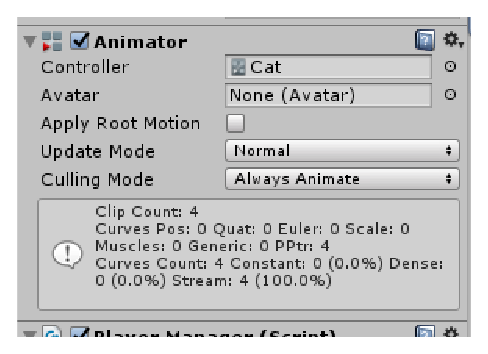
\includegraphics[width=0.3 \textwidth]{05TrabajoRealizado/03Unity/imagenes/02AnimatorGAtos}}
   
 	\subfigure[Configuracion del componente BoxCollider2D (Autoría propia).] {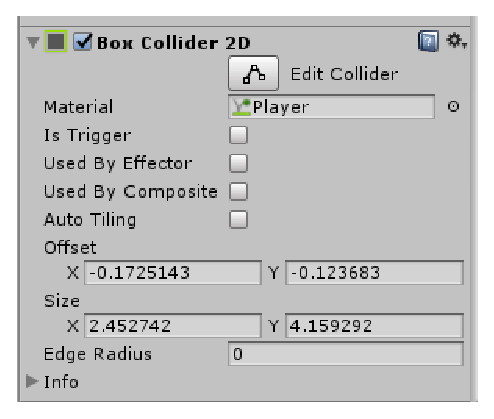
\includegraphics[width=0.3 \textwidth]{05TrabajoRealizado/03Unity/imagenes/02BoxColiderGAtos}}
 	
\subfigure[Configuracion del componente RigidBody2D (Autoría propia).] {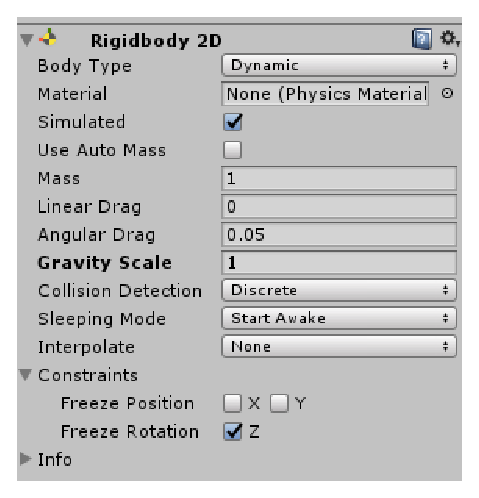
\includegraphics[width=0.3 \textwidth]{05TrabajoRealizado/03Unity/imagenes/02RigidBGAtos}}
  \caption{Componentes del Personaje jugable.}
  \label{figPersonajeJuCom}
\end{figure} 

Las animaciones del personaje jugable se gestionaron a través de una maquina de 
estados (ver figura \ref{figMaqEsCat}). Las transiciones de la maquina de 
estados son controladas por la clase PlayerManager, quien se vale del componente 
Animator para hacer dichas transiciones.

\begin{figure}
  \centering
   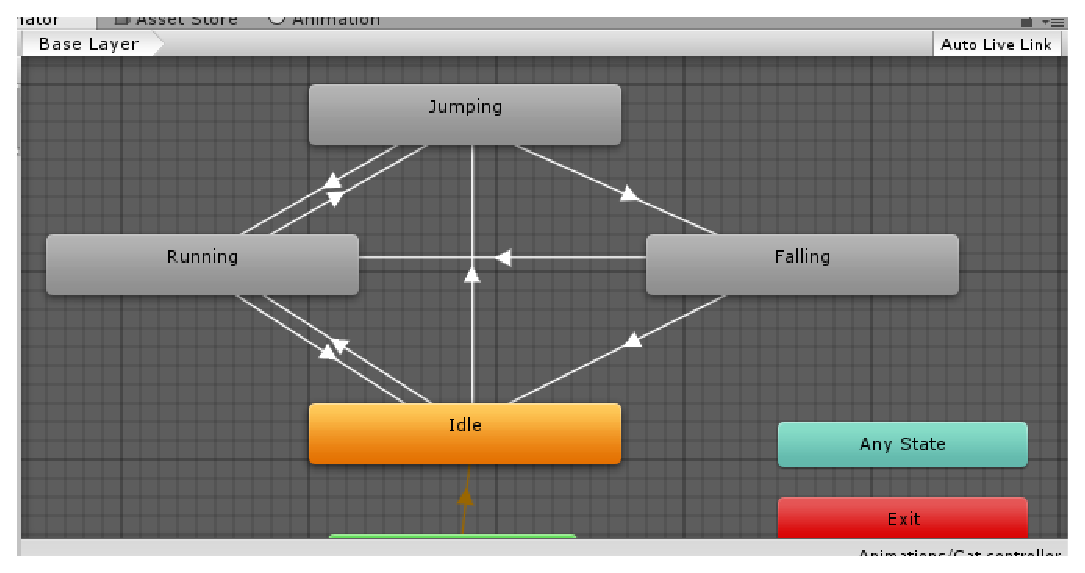
\includegraphics[width=0.6 \textwidth]{05TrabajoRealizado/03Unity/imagenes/02AnimacionGato}
  \caption{Maquina de estados del personaje jugable del prototipo 1 (Autoría propia).}
  \label{figMaqEsCat}
\end{figure} 

PlayerManager contiene casi los mismos tributos y métodos que la clase Player. 
Pero, es importante recalcar que PlayerManager no dispone de los atributos 
correspondientes a la cantidad de vida disponible ni a la cantidad de 
\textit{Tonalli}. Una de las diferencias más significativas entre ambas clases es que 
PlayerManager instancía en algunos de sus métodos clases de tipo controlador 
para utilizar métodos de estas clases (Ver figura \ref{figInstanciaCtrl}), 
mientras que la clase Player respeta la jerarquía de clases y al ser una clase de 
tipo actora no puede modificar a un controlador. En cuanto a la funcionalidad que 
tienen en común; al igual que la clase Player, PlayerManager permite al personaje jugable desplazarse de manera horizontal, saltar y disparar. Para garantizar que el método de Fire funcione, fue necesario crear un GameObject para el disparo. A éste 
GameObject se le agregaron los componentes: RigidBody2D, para el control de fisicas 
y movimiento; CircleCollider2D, para la detección de colisiones; y dos clases BulletCtrl 
y DestroyWithDelay.
\\
\par
 
\begin{figure}
  \centering
   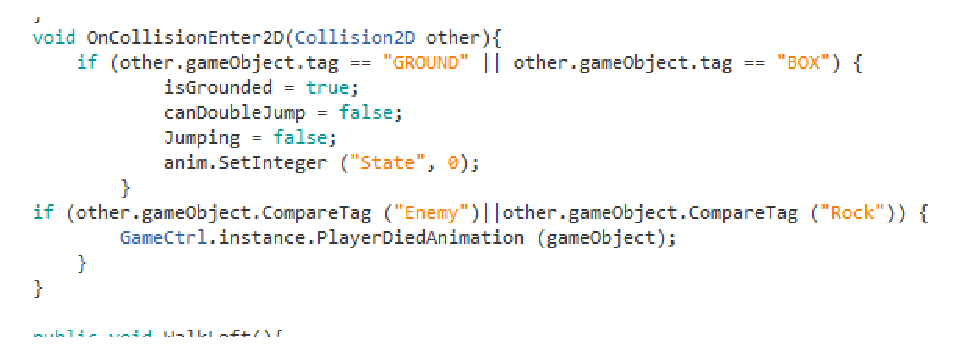
\includegraphics[width=0.6 \textwidth]{05TrabajoRealizado/03Unity/imagenes/02GatoCtrl}
  \caption{PlayerManager instancia clase de tipo controlador para actualizar marcadores (Autoría propia)}
  \label{figInstanciaCtrl}
\end{figure} 


En cuanto a la detección y respuesta de colisiones, la clase PlayerManager se 
vale de la capacidad de Unity para etiquetar objetos. Bajo este sistema de 
etiquetación se puede determinar una respuesta en concreto a todos los objetos 
que colisionen con el personaje jugable y que compartan una misma etiqueta. A 
continuacion se listan algunas de la etiquetas que se manejaron en este prototipo, 
seguida de la respuesta del personaje jugable al colisionar con un 
objeto bajo esta etiqueta:
\begin{itemize}
	\item \item Ground: PlayerManager actualiza atributos que habilitan la capacidad 
	de usar el método Jump y de que estado de animación activar cuando el personaje 
	jugable se mueva.
	\item Enemy: PlayerManager instancía la clase GameCtrl y le pide que ejecute el 
	método PlayerDiedAnimation para indicar la muerte del personaje jugable (ver 
	figura \ref{figPersonajeResEne}).
	\item Dog: PlayerManayer instancía la clase GameCtrl y le pide que ejecute el 
	método UpdateXoloCount, despues destruye el objeto con la etiqueta Dog 
	y en su posición muestra un efecto especial de brillos. 
\end{itemize} 

\begin{figure}
  \centering
  
   \subfigure[Personaje Jugable antes de colisión con enemigo (Autoría propia).] {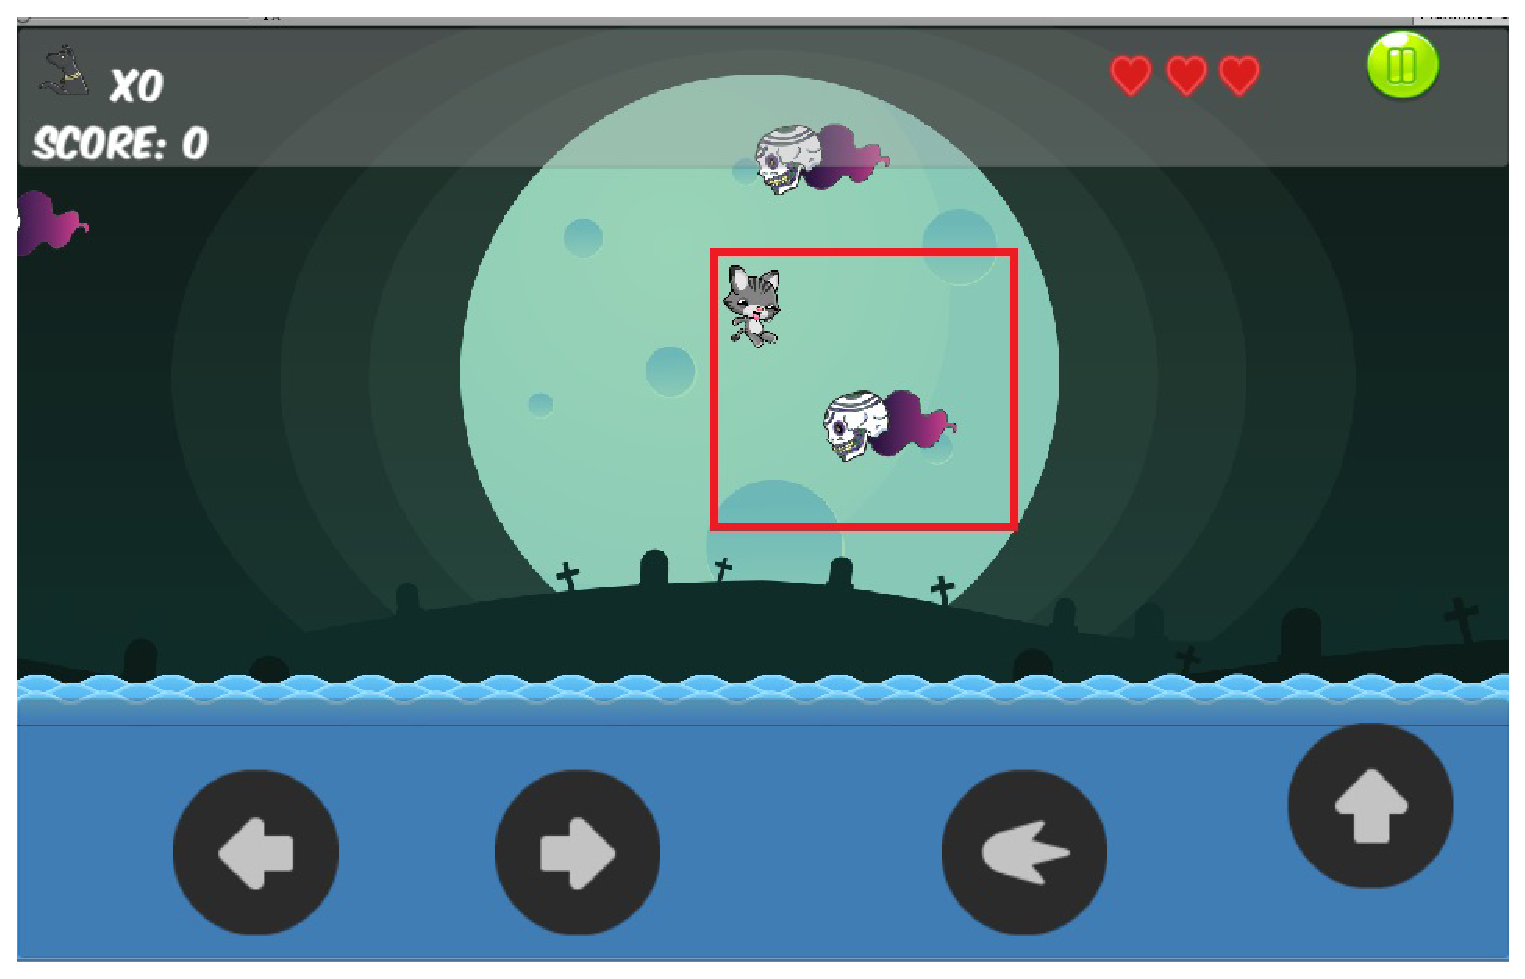
\includegraphics[width=0.4 \textwidth]{05TrabajoRealizado/03Unity/imagenes/02reaccionColisionEnemi01}}
   
 	\subfigure[Ejecución del método PlayerDiedAnimation (Autoría propia).] {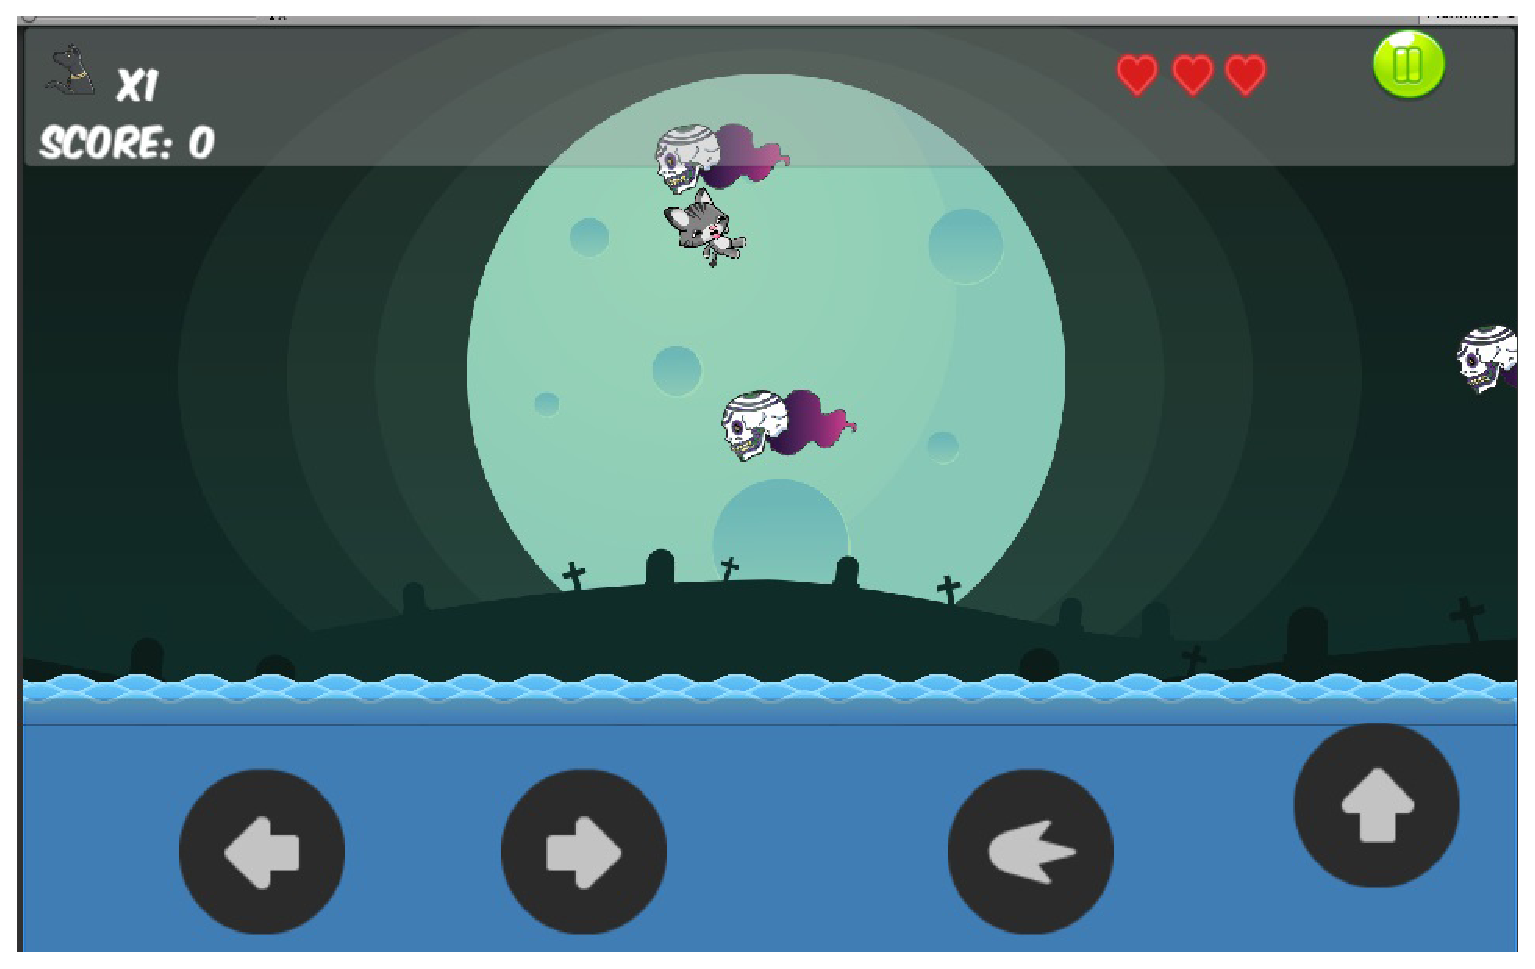
\includegraphics[width=0.4 \textwidth]{05TrabajoRealizado/03Unity/imagenes/02reaccionColisionEnemi02}}
 	
\subfigure[Actualización de la cantidad de vidas después de reiniciar el nivel tras colisión con el enemigo (Autoría propia).] {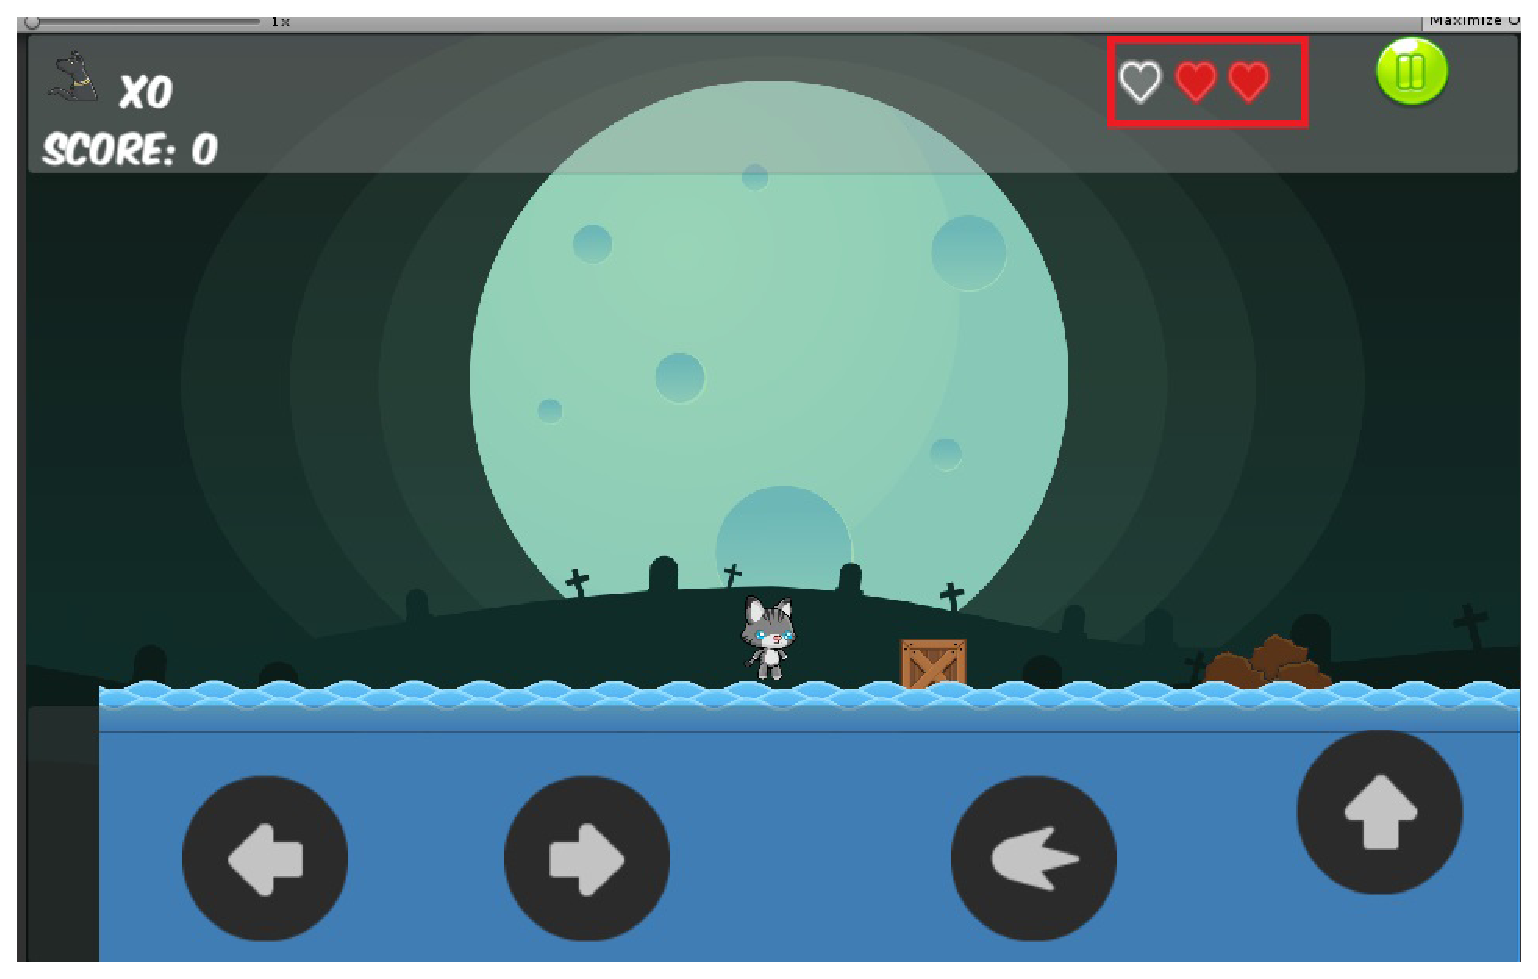
\includegraphics[width=0.4 \textwidth]{05TrabajoRealizado/03Unity/imagenes/02reaccionColisionEnemi03}}

  \caption{Respuesta visual del juego cuando el personaje jugable colisiona con un enemigo.}
  \label{figPersonajeResEne}
\end{figure} 

\begin{figure}
  \centering
  
   \subfigure[Personaje Jugable antes de colisión con xoloitzcuintle (Autoría propia).] {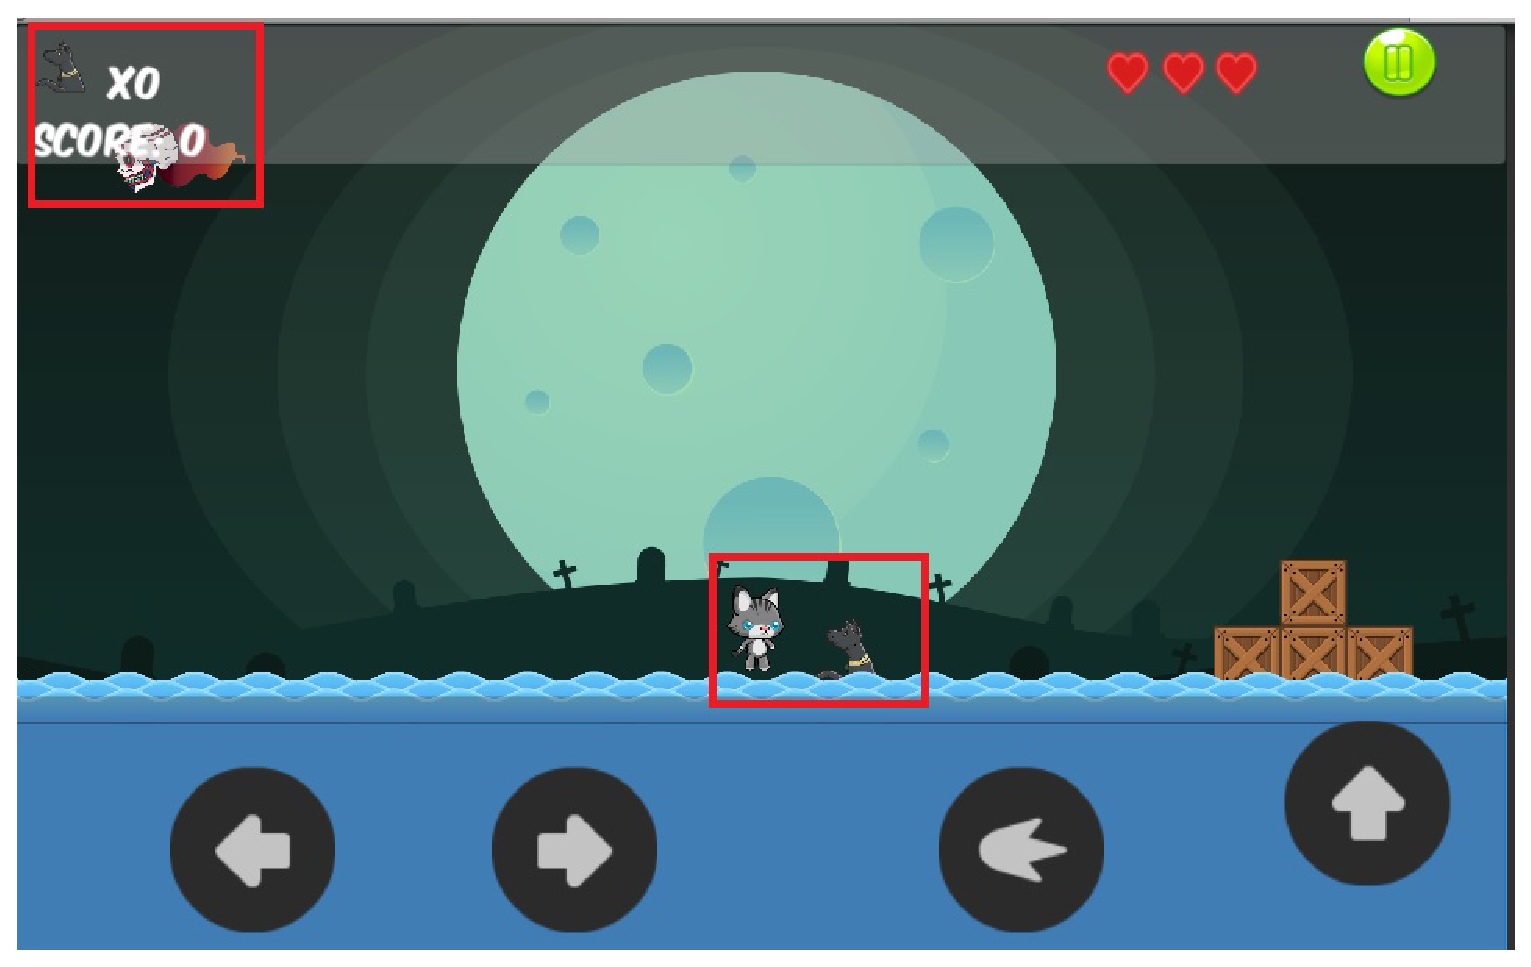
\includegraphics[width=0.4 \textwidth]{05TrabajoRealizado/03Unity/imagenes/02reaccionColisionperro01}}
   
 	\subfigure[Actualización del marcador de xoloitzcuintles (Autoría propia).] {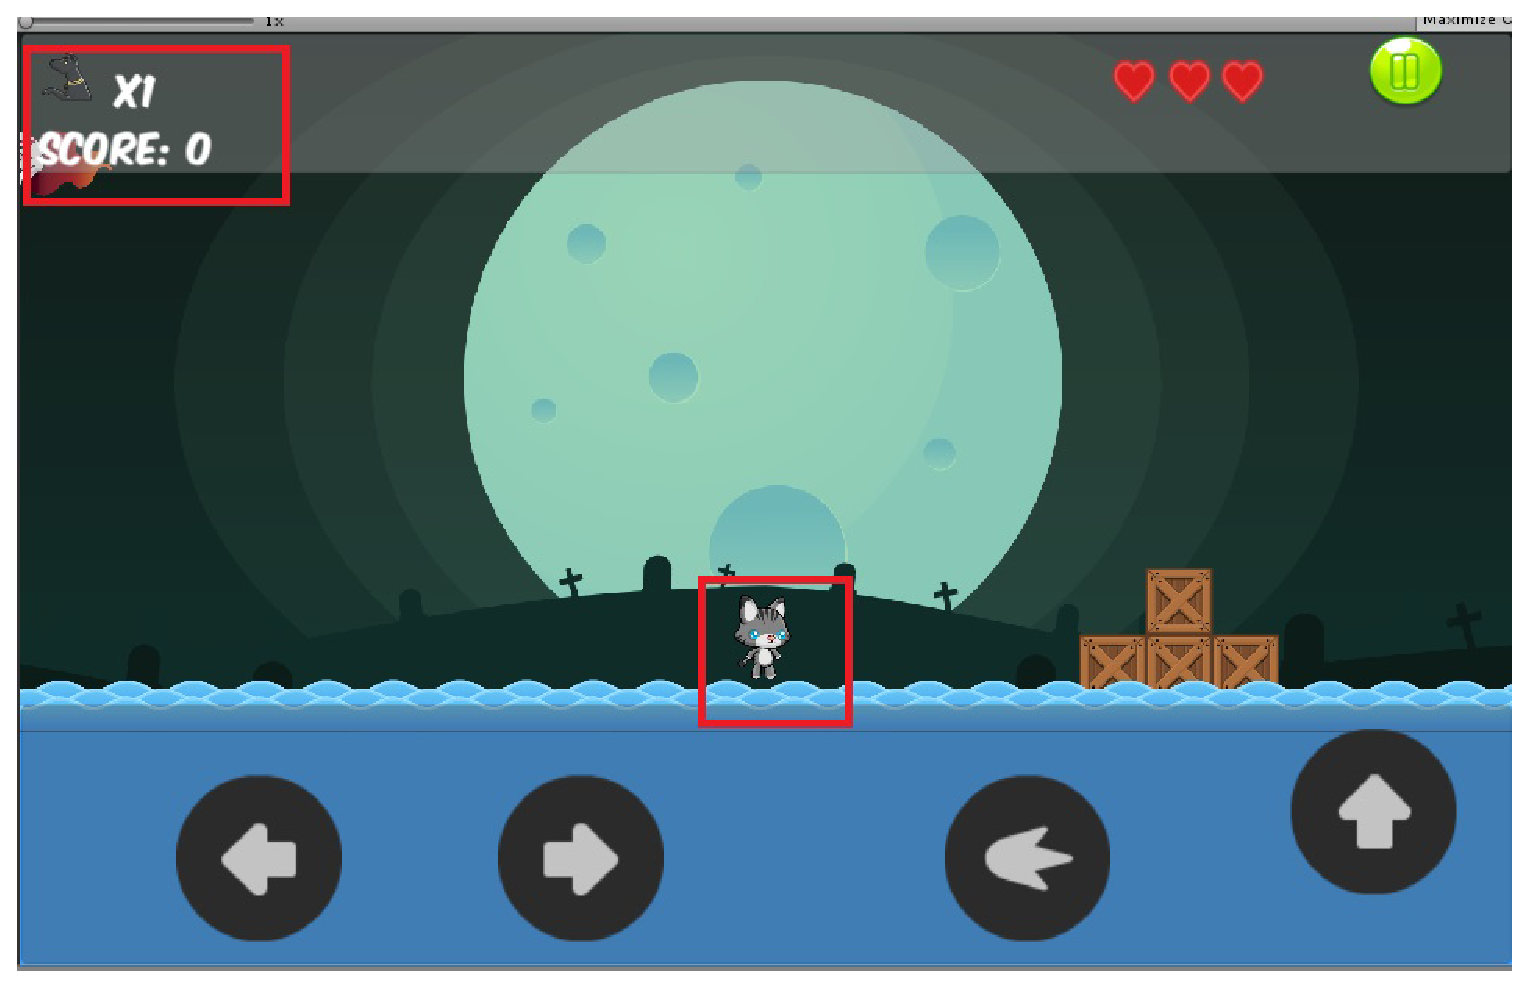
\includegraphics[width=0.4 \textwidth]{05TrabajoRealizado/03Unity/imagenes/02reaccionColisionperro02}}

  \caption{Respuesta visual del juego cuando el personaje jugable colisiona con un xoloitzcuintl.}
  \label{figPersonajeResXo}
\end{figure} 

\subsubsection{Implementar Interfaz gráfica} 
La interfaz gráfica se compone de dos canvas: uno para para los botones que 
controlan al juagdor y otro para mostrar los marcadores y numero de vidas del 
jugador (Ver figura \ref{figCanvas}).
\\
 \par
\begin{figure}
  \centering
   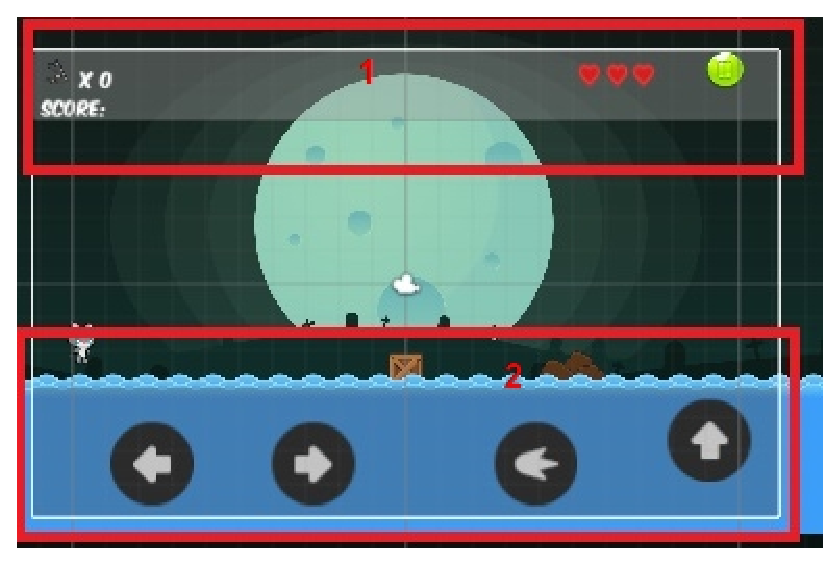
\includegraphics[width=0.4 \textwidth]{05TrabajoRealizado/03Unity/imagenes/02ConfiguracionCanvas02}
  \caption{La interfaz gráfica se divide en dos partes: 1. Canvas que muestra maracadores. 2. Canvas que contiene los botones que controlan al juagador(Autoría propia)}
  \label{figCanvas}
\end{figure} 

Ambos Canvas son configurados para que su tamaño se ajuste al objeto camara; de
 igual manera se configura su escalamiento para que su tamaño se adapte al de la
  pantalla que se tenga disponible evitando que los componentes del canvas 
  adquieran un tamaño que imposibilite el control del personaje jugable o la 
  visualización de información (ver figura \ref{figCanvasConf}).    
 \\
 \par
 \begin{figure}
  \centering
   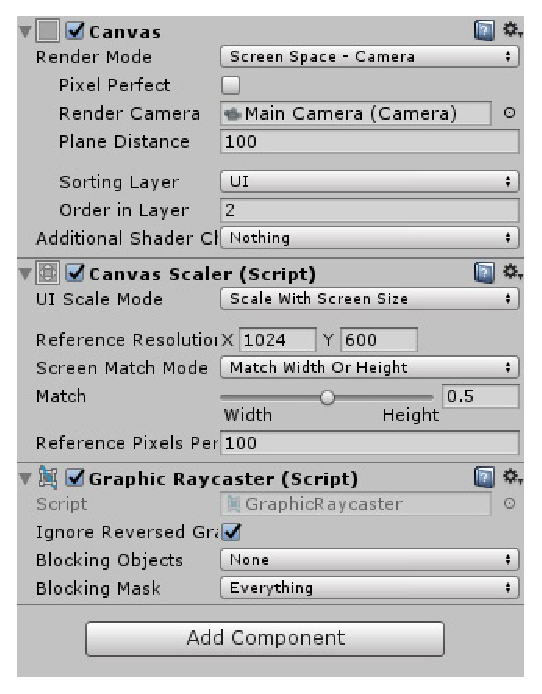
\includegraphics[width=0.4 \textwidth]{05TrabajoRealizado/03Unity/imagenes/02ConfiguracionCanvas}
  \caption{Configuración del canvas para que su tamaño sea el adecuado aun si el tamaño de pantalla cambia (Autoría propia)}
  \label{figCanvasConf}
\end{figure}
 El canvas que corresponde al conteo de vidas y al marcador es controlado por  
 la clase GameCtrl. Mientras que el canvas referente a los botones obtiene su  
 funcionalidad de la clase MobileUICtrl para comunicar al jugador con la clase 
 PlayerManager y con el personaje jugable.  
 
 \subsubsection{Manejo de un score para el juego y preservación de datos de la partida}
Como se mencionó con anterioridad, el marcador es controlado por la clase GameCtrl. 
Esta clase es el equivalente a la fusion de las clases LevelCtrl y DataFile 
descritas en el apartado \ref{ClasesJuego}. Al igual que como ocurre con Player 
y PlayerManager, GameCtrl y LevelCtrl y DataFile tienen métodos y atributos 
comunes. La diferencia más importante entre estas clases es que GameCtrl solo 
permite el almacenamiento de información para controlar un nivel y no puede 
gestionar la transición entre escenas. 
\\
\par
En cuanto al manejo del marcador, este se actualiza cada vez que el personaje jugable 
colisiona con un ojeto bajo la etiqueta Dog (ver figura \ref{figPersonajeResXo}) o el 
Jugador logra derrotar a un enemigo (ver figura ). En cada actualización del marcador, 
GameCtrl almacena los datos de la partida en un archivo de tipo binario. Cuando el 
personaje colisiona con un enemigo, GameCtrl permite mantener los valores de los 
maracadores y cantidad de vida del jugador, más no la posición que este tenía antes 
de la colisión.   
 
\begin{figure}
  \centering
  
   \subfigure[Personaje Jugable antes de disparar a enemigo (Autoría propia).] {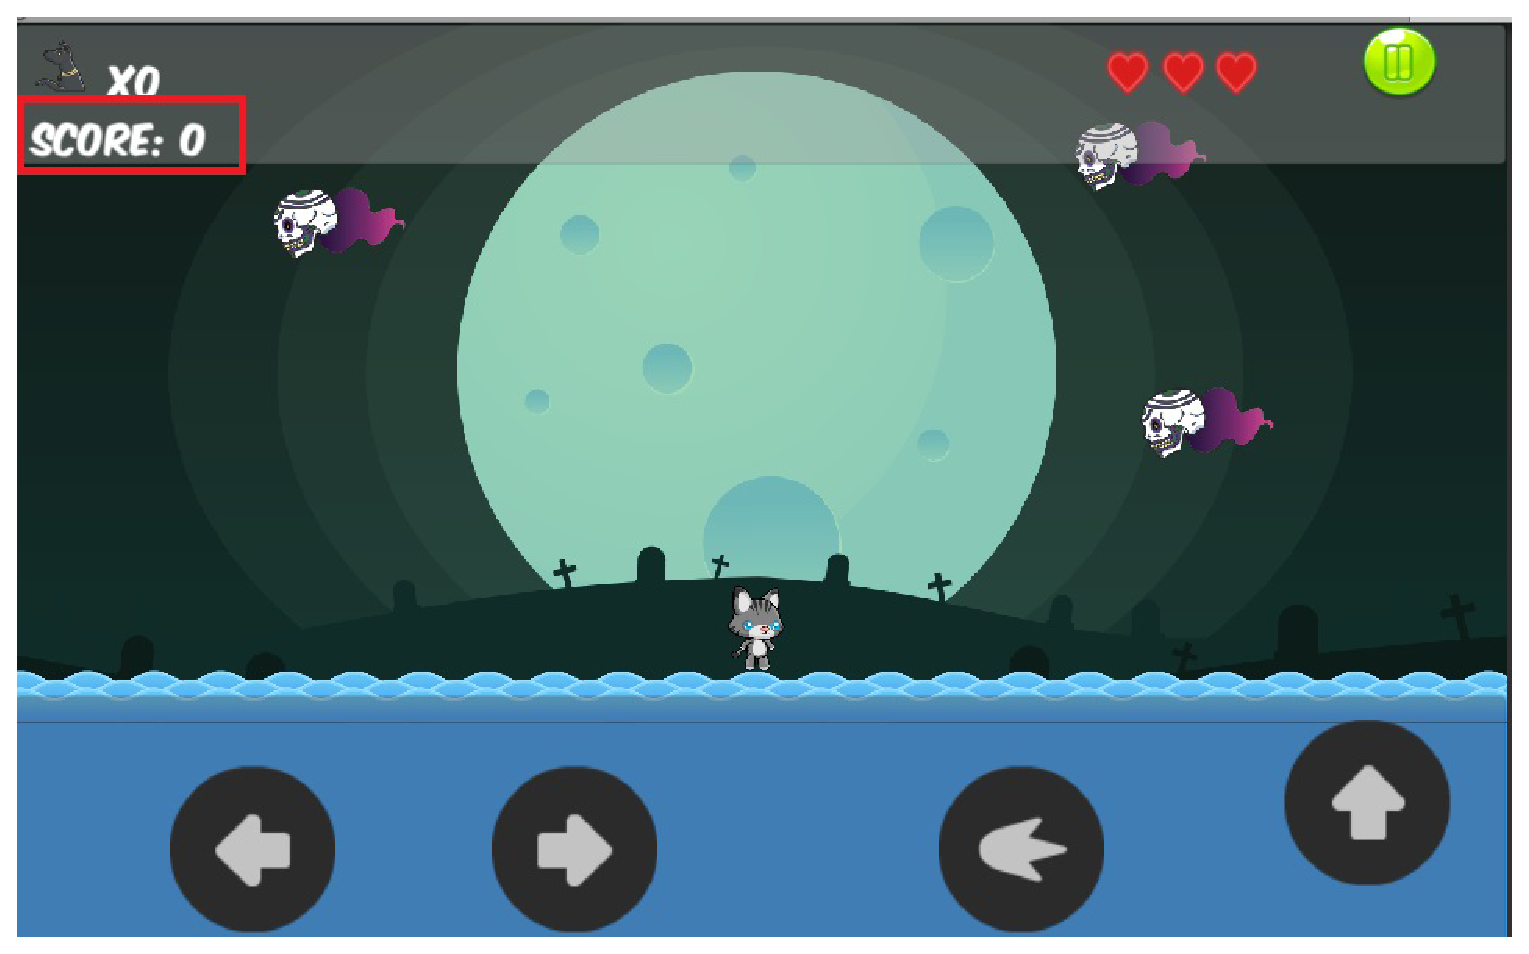
\includegraphics[width=0.4 \textwidth]{05TrabajoRealizado/03Unity/imagenes/02reaccionScore03}}
   
 	\subfigure[Actualización de marcador al derrotar a un enemigo (Autoría propia).] {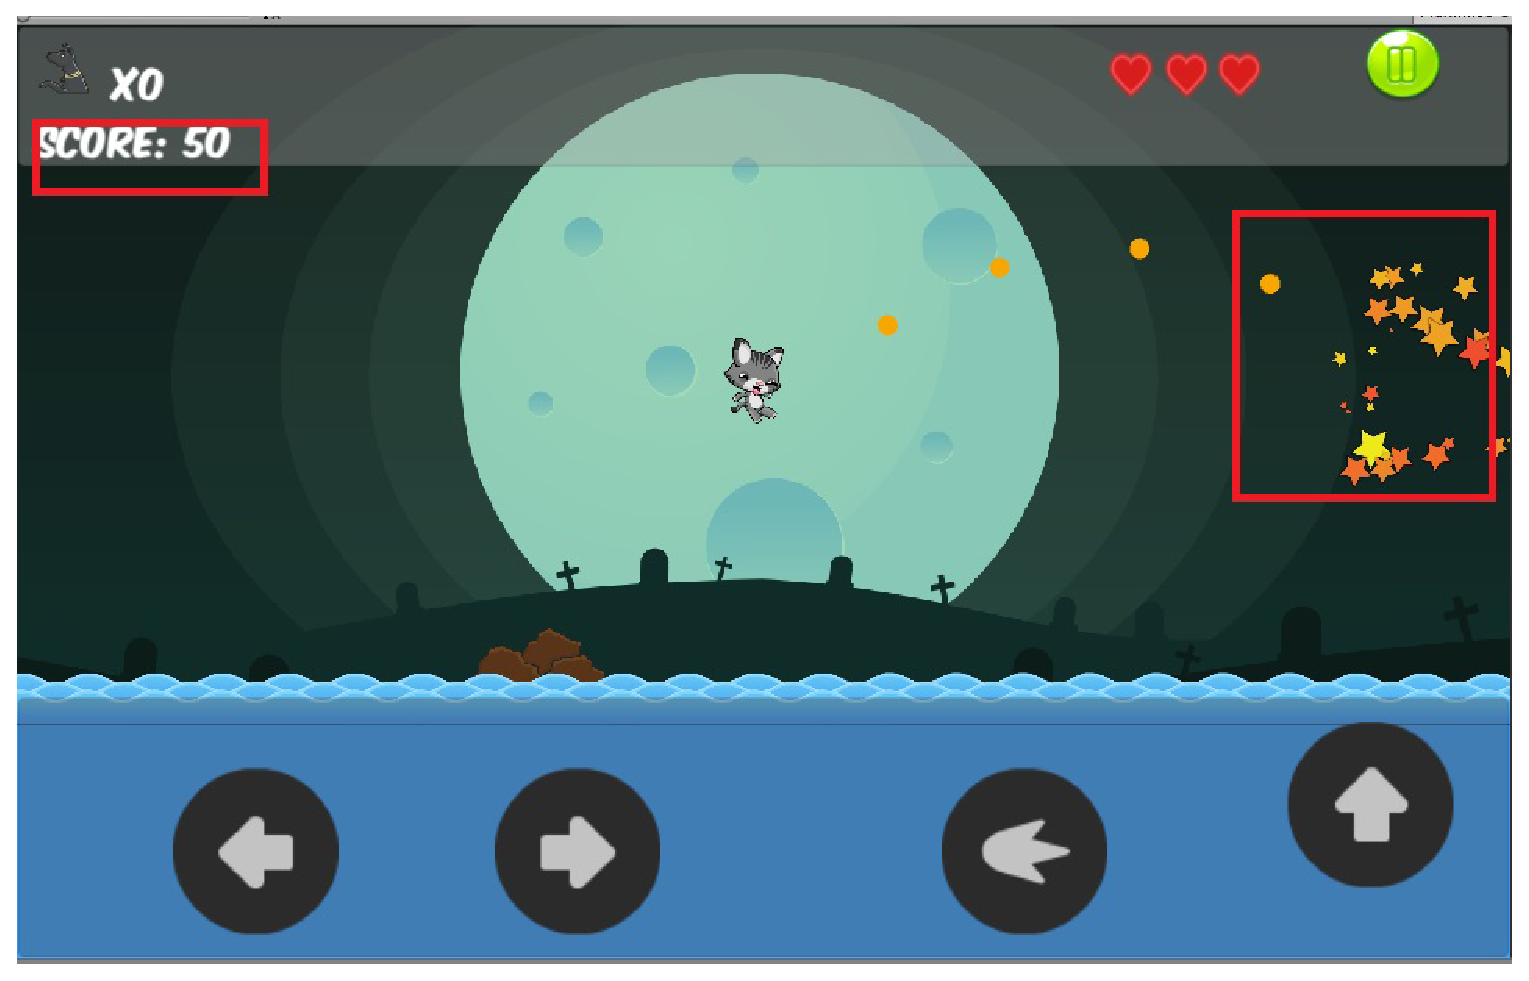
\includegraphics[width=0.4 \textwidth]{05TrabajoRealizado/03Unity/imagenes/02reaccionScore02}}

  \caption{Respuesta visual del juego cuando el personaje jugable derrota a un enemigo.}
  \label{figPersonajeResXo}
\end{figure}     
 
 \subsubsection{Patron de movimiento para los enemigos}
 Para la creación de los patrones de movimiento de los enemigos fue necesario  
 crear tres GameObjects vacíos para el enemigo de tipo PurpleGost(ver figura ) y dos 
 GameObjects vacíos para el enemigo de tipo RedGost. Utilizando la posición de los 
 GameObjects vacios cada tipo de enemigo sigue el patrón de movimiento desctrito en las 
 figura \ref{figPurpleGost} y \ref{figRedGost}.  

\begin{figure}
  \centering
   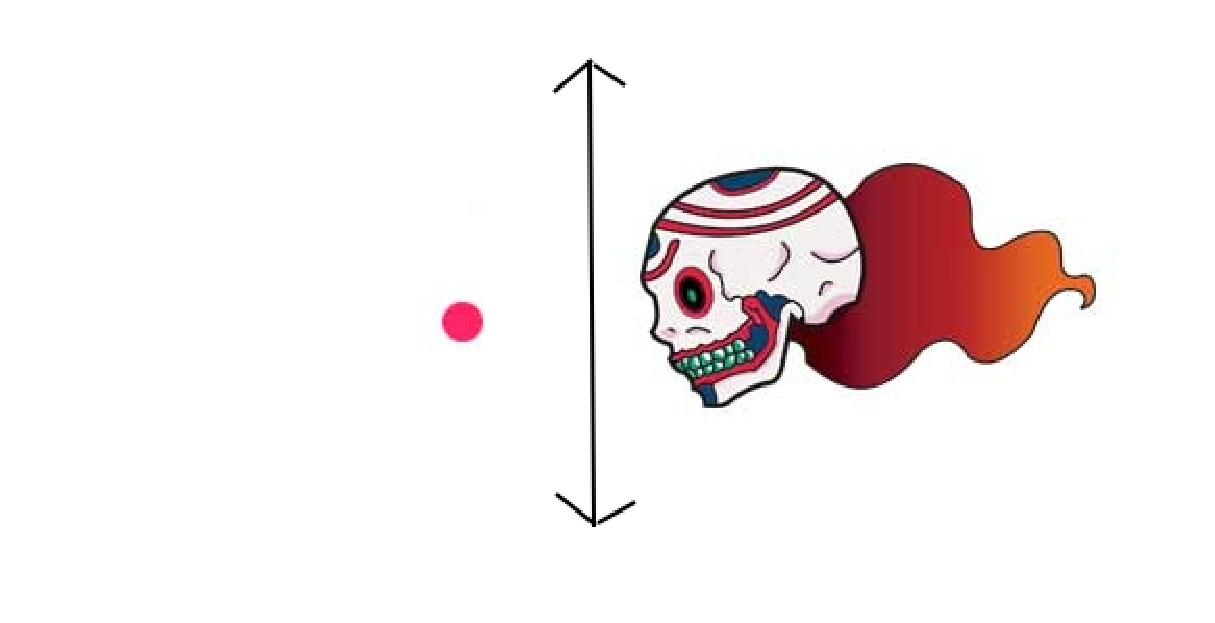
\includegraphics[width=0.4 \textwidth]{05TrabajoRealizado/03Unity/imagenes/disparoRojo}
  \caption{Patrón de movimiento de RedGost (Autoría propia)}
  \label{figRedGost}
\end{figure}

\begin{figure}
  \centering
   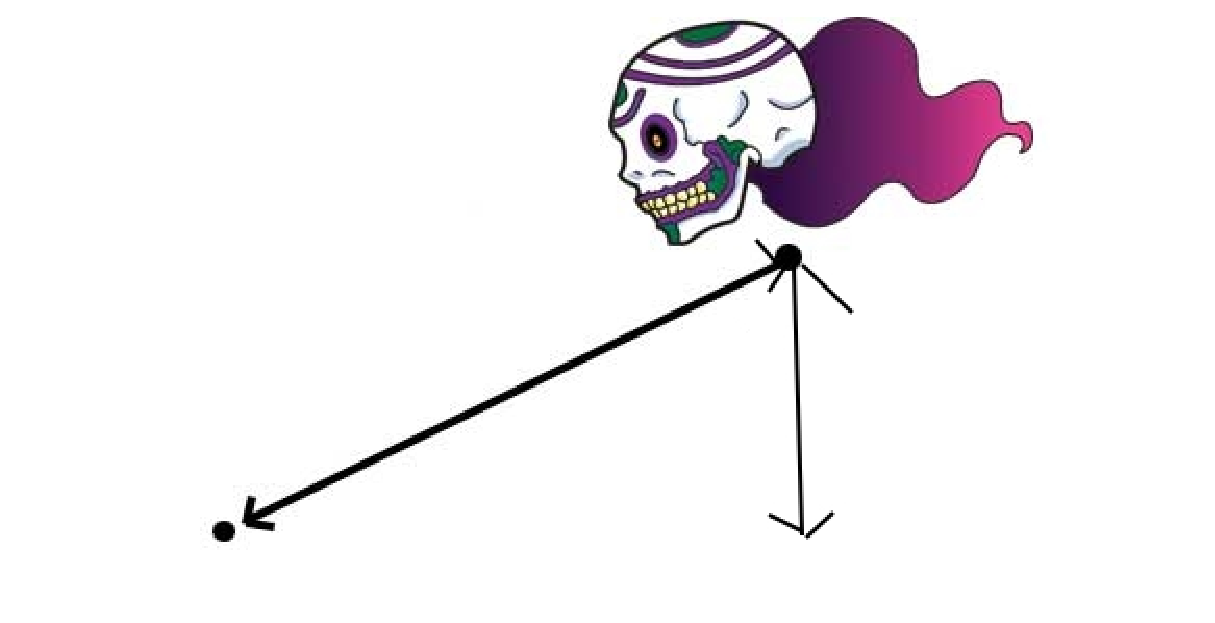
\includegraphics[width=0.4 \textwidth]{05TrabajoRealizado/03Unity/imagenes/embestida}
  \caption{Patrón de movimiento de PurpleGost (Autoría propia)}
  \label{figPurpleGost}
\end{figure}
\subsection{Segundo Prototipo}
El segundo prototipo modela el comportamiento del primer nivel del juego (ver 
apartado \ref{Niveles}). 

\subsubsection{Creación de Sprites}
Para este prototipo se crearon todos los sprites a utilizar, salvo por los botones 
de la Interfaz de usuario, ya que estos se conservaron del prototipo anterior. En 
total se crearon:
\begin{itemize}
	\item Tres imágenes de fondo.
	\item Tres íconos.
	\item Diez imágenes para la animación de Malinalli.
	\item Seis imágenes para la animación de Xólotl en su forma xoloitzcuintle.
	\item Seis imágenes para la animación de Xólotl en su forma humano.
	\item Una imagen para Quetzalcóatl.
	\item Cinco imágenes para los ciudadanos
	\item Cuatro imágenes para el suelo.
	\item Cuatro imágenes para los objetos de fondo de la ciudad.
	\item Dos imágenes para los objetos de fondo de la jungla.
	\item Cinco imágenes para la animación del Jaguar.
\end{itemize}  
Consultar \ref{SpriteDic} para ver el resto de los sprites creados.

\subsubsection{Menú principal}
En este apartado se modificó la propuesta de diseño que se tenía en las interfaces 
(ver apartado \ref{TraReaInterfaces}). Tal como se puede ver en la figura 
\ref{figDisenioMenu}, la posición de los botones del prototipo varía con 
respecto a la del diseño. 
\\
\par
Al igual que en el prototipo uno, se configuraron los botones y el 
canvas para que adapten su tamaño si se modifica el tamaño de la 
pantalla.
\\
\par
Para la funcionalidad del menú principal se implementó la clase PrincipalMenuCtrl; 
sin embargo, no se implementaron todos sus métodos ni todos sus atributos. Siendo 
el botón Empezar partida, él unico con la funcionalidad parcialmente habilitada, 
ya que al ser oprimido por el jugador solo realiza la transición de la interfaz del 
menu principal a la primera mitad del nivel uno sin generar el archivo de datos 
de partida.
\\
\par

\begin{figure}
  \centering
   \subfigure[Propuesta de diseño para la interfaz del menú principal (Autoría propia).] {\includegraphics[width=0.4 \textwidth]{05TrabajoRealizado/03Unity/imagenes/interfaz01}}
   
 	\subfigure[Diseño final del menú principal (Autoría propia).] {\includegraphics[width=0.4 \textwidth]{05TrabajoRealizado/03Unity/imagenes/menuPrincipalFinal}}
 	
  \caption{La implementación del menu principal varía la posición de los botones con respecto a la propuesta de diseño.}
  \label{figDisenioMenu}
\end{figure} 

\subsubsection{Implementación personaje jugable}
En cuanto a la implementación del personaje jugable, se trató de reutilizar la lógica 
del primer prototipo, con algunas diferencias. A continuación
se listan los cambios más significativos con respecto a la clase del prototipo anterior:
\begin{itemize}
	\item La clase \textit{Player} y la clase \textit{GroundCollisionCtrl} son las 
	encargadas de la funcionalidad del personaje jugable.
	\item La clase \textit{Player} deja de instanciar clases de tipo Controlador.
	\item El estado \textit{Idle} de la maquina de estados se renombra como
	 \textit{Normal} (ver Figura \ref{figMaqMalinalli}).
	 \item El sprite del personaje jugable corresponde con el diseño del personaje 
	 principal del juego propuesto en el documento de diseño (ver figura \ref{figAniMalinalli})
	 \item Se manejan atributos de tipo boolean como banderas de 
	 activación en los métodos que vinculan la clase \textit{Player} con la clase 
	 \textit{MobileUICtrl}.
\end{itemize}

\begin{figure}
  \centering
   \includegraphics[width=0.4 \textwidth]{05TrabajoRealizado/03Unity/imagenes/03MaquinaEstadosMalinalli}
  \caption{Máquina de estados para la animación del personaje jugable Malinalli (Autoría propia)}
  \label{figMaqMalinalli}
\end{figure}

\begin{figure}
  \centering
   \includegraphics[width=0.4 \textwidth]{05TrabajoRealizado/03Unity/imagenes/bloquesanimacionMalinalli}
  \caption{Animacion de Run y Jump del personaje jugable Malinalli (Autoría propia)}
  \label{figAniMalinalli}
\end{figure}

\subsubsection{Interfaz gráfica del nivel}
Al igual que el prototipo anterior, la interfaz gráfica se compone de dos canvas: uno 
para los marcadores y otro para los botones que permiten al jugador controlar al personaje jugable (Ver figura \ref{figCanvasM}).
\\
\par
El canvas que contiene a los botones se mantinen si cambios referentes a su 
visualización; no obstante, los métodos de la clase Player que se activan con 
estos varían. En este nivel el método FireGUI de la clase MobileUICtrl se 
remplaza por el método de GUIStartConversation de la clase TalkedCharacter; no 
obstante todas las clases referentes a la lectura y activación de dialogos no 
fueron implementadas por lo que el Botón de disparo se encuentra sin funcionalidad.
\\
\par
Por su parte el canvas que contiene los marcadores modifica su estructura visual (ver 
figuar \ref{figCanvasM}). Los corazones que indicaban la cantidad de vidas del 
prototipo anterior por una barra de vida y se agrega por primera vez la  
barra de cantidad Tonalli.   

\begin{figure}
  \centering
   \includegraphics[width=0.4 \textwidth]{05TrabajoRealizado/03Unity/imagenes/03Interfaz}
  \caption{La interfaz gráfica se encuetra compuesta por dos canvas: 1. Contenedor de los marcadores. 2. Contenedor de los botones que permiten el control al personaje jugable (Autoría propia)}
  \label{figCanvasM}
\end{figure}

\subsubsection{Primer mitad del nivel uno}
Tomando la maqueta del primer nivel como base, se crearon los GameObjects 
correspondientes para construir la primera parte del primer nivel (ver \ref{Mac01}). 
 En esta primera mitad del prototipo no se alcanzó a crear la clase DialogueCtrl y todas sus clases ligadas por lo que se creó un GameObject vació, se le agregó el componente Box Collider2D, y se agrego una  de este modo se realiza la transición a la segunda mitad del primer nivel.
 
 \subsubsection{Segunda mitad del primer nivel}
 En esta segunda mitad se implementó la clase FollowedCharacter para la persecución 
 de Xólotl en su forma xoloitzcuintle. En Xólotl también fue necesario implementar 
 una maquina de estados para sus animación. Como se puede ver en la figura \ref{figAniXolo} la  máquina de estados de Xólotl esta compuesta de dos estados: .
 
 \begin{figure}
  \centering
   \includegraphics[width=0.4 \textwidth]{05TrabajoRealizado/03Unity/imagenes/03MaquinaEstadosXolotl}
  \caption{Máquina de estados de Xólotl forma xoloitzcuintle (Autoría propia)}
  \label{figAniXolo}
\end{figure}
		

	%\input{05TrabajoRealizado/04ProgramacionNiveles}
		
	\chapter{Resultados obtenidos}
Al término del desarrollo del Trabajo Terminal 1 se obtuvieron los siguientes 
productos:
	\begin{itemize}
		\item Documento de diseño.
		\item Guión literario del juego.
		\item Diseños de todos los personajes.
		\item Diseños de todas las armas del juego.
		\item Diseños de todos los items.
		\item Bosquejo conceptual de las habilidades de los personajes.
		\item Definicón de las clases que componen el juego.
		\item  Sprites del primer nivel.
		\item Maqueta del primer nive.
		\item Maqueta del segundo nivel. 
	\end{itemize}
	\chapter{Reflexiones}

% punto final del informe: "como ha sido mostrado...."

Como se vió durante el avance del proyecto, 
un videojuego educativo es una gran herramienta de ayuda para la enseñanza y el aprendizaje. Este es un medio controlado con normas establecidas, lo que facilita en control de información y en que modo debe aprenderse.

La cultura puede ser vista como entretenida gracias al juego. Se puede combinar de manera digerible por el jugador los componentes históricos y de juego. Y este tipo de combinación en material cultural con un videjuego es bien recibido por casi todos los diferentes tipos de personas.

La intención es que con los incentivos correctos para grupos específicos de personas, en este caso un videojuego, se pueda motivar a la sociedad a que se interese y aprenda conocimiento cultural. 

	\printbibliography
	\chapter{Anexos}
\section{Sprites}\label{SpriteDic}
En esta seccion se muestran algunos de los sprites que se crearon para los 
personajes y los fondos. 
\subsection{Imagenes de Fondo}
En esta sección de muestran las imagenes para los fondos del juego que se crearon:
\\
\par
\begin{center}
\includegraphics[width=0.6\textwidth]{09Anexos/sprites/fondo02}
\end{center}

\begin{center}
\includegraphics[width=0.6\textwidth]{09Anexos/sprites/fondo-Mont}
\end{center}

\begin{center}
\includegraphics[width=0.6\textwidth]{09Anexos/sprites/yolotl_logo}
\end{center}

\subsection{Personajes}
En esta sección de muestran algunas de las imagenes para los personajes del juego que se crearon:
\\
\par
\begin{center}
\includegraphics[width=0.3\textwidth]{09Anexos/sprites/mujer02}
\end{center}

\begin{center}
\includegraphics[width=0.1\textwidth]{09Anexos/sprites/muujer01}
\end{center}

\begin{center}
\includegraphics[width=0.7\textwidth]{09Anexos/sprites/xolotlAnimacion}
\end{center}
\section{Maquetas}
En esta sección se muestran las maquetas referentes al nivel 1 y al nivel 2.

\subsection{Maqueta nivel 1}\label{Mac01}
Maquetado del nivel 21.
\begin{center}
\includegraphics[width=0.9\textwidth]{09Anexos/sprites/M0101}
\end{center}

\begin{center}
\includegraphics[width=0.9\textwidth]{09Anexos/sprites/M0102}
\end{center}

\begin{center}
\includegraphics[width=0.9\textwidth]{09Anexos/sprites/M0103}
\end{center}

\begin{center}
\includegraphics[width=0.9\textwidth]{09Anexos/sprites/M0104}
\end{center}

\begin{center}
\includegraphics[width=0.9\textwidth]{09Anexos/sprites/M0105}
\end{center}


\subsection{Maqueta nivel 2}\label{Mac02}
Maquetado del nivel 2.
\begin{center}
\includegraphics[width=0.9\textwidth]{09Anexos/sprites/ML0201}
\end{center}

\begin{center}
\includegraphics[width=0.9\textwidth]{09Anexos/sprites/ML0202}
\end{center}

\begin{center}
\includegraphics[width=0.9\textwidth]{09Anexos/sprites/ML0203}
\end{center}

\begin{center}
\includegraphics[width=0.9\textwidth]{09Anexos/sprites/ML0204}
\end{center}

\begin{center}
\includegraphics[width=0.9\textwidth]{09Anexos/sprites/ML0205}
\end{center}

\begin{center}
\includegraphics[width=0.9\textwidth]{09Anexos/sprites/ML0206}
\end{center}

\begin{center}
\includegraphics[width=0.9\textwidth]{09Anexos/sprites/ML0207}
\end{center}

\begin{center}
\includegraphics[width=0.9\textwidth]{09Anexos/sprites/ML0208}
\end{center}

\begin{center}
\includegraphics[width=0.9\textwidth]{09Anexos/sprites/ML0209}
\end{center}

\begin{center}
\includegraphics[width=0.9\textwidth]{09Anexos/sprites/ML0210}
\end{center}
\section{Cronograma de actividades} cron
En esta sección se muestra el cronograma de actividades de la metodología huddle.

\begin{center}
\includegraphics[width=1\textwidth]{09Anexos/sprites/crono01}
\end{center}

\begin{center}
\includegraphics[width=1\textwidth]{09Anexos/sprites/crono02}
\end{center}

\begin{center}
\includegraphics[width=1\textwidth]{09Anexos/sprites/crono03}
\end{center}

	
\end{document}